\documentclass[compress,10pt,aspectratio=169]{beamer}

%%%%%%%%%%%%%%%%%%%%%%%
% Thème beamer ONERA :
% Options :
%%%%%%%%%%%%%%%%%%%%%%%
%     - english -> biblio en anglais [défaut en français]
%	  (se sert de la mise en forme bibliographique onera.bst de Frédéric Cassaing (Frederic.Cassaing@onera.fr)
%	  (+url de la page de remerciement renvoie vers le site ONERA en anglais [défaut renvoie sur le site en français]).
%     - customnumbering -> permet d'afficher la numérotation des diapositives de manière élégante.
%	  (/!\ la compilation peut être longue avec cette option si il y a beaucoup de diapositives ! Il vaut mieux alors compiler sans l'option
%	   puis compiler une fois les diapositives finalisées).
%     - DR, CD, SD, S, TS -> ajout de la mention 'DIFFUSION RESTREINTE' ou 'CONFIDENTIEL DEFENSE' ou 'SECRET DEFENSE' ou 'SECRET' ou 'TRES SECRET'(rouge) dans le footer de la présentation. (Note, il ne faut choisir qu'une seule mention à la fois!)
%     - SF -> ajout de la mention 'SPECIAL FRANCE' (bleu) dans le footer de la présentation
%\usetheme[customnumbering]{onera}
\usetheme[english]{onera}


%%%%%%%%%%%%%%%%%%%%%%%
% Packages additionnels
%%%%%%%%%%%%%%%%%%%%%%%
\usepackage{amsmath,amssymb,amsfonts}
\usepackage{stmaryrd}
\usepackage{multirow}
\usepackage{bbold}
\usepackage{epsfig}
\usepackage{ulem}
\usepackage{comment}
\newcommand{\thicktilde}[1]{\mathbf{\tilde{\text{$#1$}}}}


\usepackage{algorithm2e}
\renewcommand{\listalgorithmcfname}{Liste des Algorithmes}%
\renewcommand{\algorithmcfname}{Algorithme}%
\renewcommand{\algorithmautorefname}{algorithme}%
\renewcommand{\algorithmcflinename}{ligne}%
%\renewcommand{\algocf@typo}{\ }%
%\renewcommand{\@algocf@procname}{Proc\'edure}%
%\renewcommand{\@algocf@funcname}{Fonction}%
\renewcommand{\procedureautorefname}{proc\'edure}%
\renewcommand{\functionautorefname}{fonction}%
%\renewcommand{\algocf@languagechoosen}{french}%

%\SetKwHangingKw{HDonnees}{Donnees$\rightarrow$}
%\SetKwInpsut{Donnees}{Donn\'ees}%
%\SetKwInput{Res}{R\'esultat}%
\SetKwInput{Entrees}{Entr\'ees}%
\SetKwInput{Entree}{Entr\'ees}%
\SetKwInput{Sortie}{Sortie}%
\SetKwInput{Sorties}{Sorties}%
%\SetKw{KwA}{\`a}%
%\SetKw{Retour}{retourner}%
%\SetKwBlock{Deb}{d\'ebut}{fin}%
\SetKwRepeat{Repeter}{r\'ep\'eter}{jusqu'\`a}%
%
\SetKwIF{Si}{SinonSi}{Sinon}{si}{alors}{sinon si}{sinon}{fin si}%
\SetKwSwitch{Suivant}{Cas}{Autre}{suivant}{faire}{cas o\`u}{autres cas}{fin cas}{fin d'alternative}%
\SetKwFor{Pour}{pour}{faire}{fin pour}%
\SetKwFor{PourPar}{pour}{faire en parall\`ele}{fin pour}%
\SetKwFor{PourCh}{pour chaque}{faire}{fin pour chaque}%
\SetKwFor{PourTous}{pour tous}{faire}{fin pour tous}%
\SetKwFor{Tq}{tant que}{faire}{fin tq}%


% Dessin (Note : le package 'tikz' est chargé par défaut avec le thème ONERA ainsi que l'option 'positioning')
\usepackage{tikz-3dplot}
\usetikzlibrary{shapes.misc}
\tikzset{cross/.style={cross out, draw=black, fill=none, minimum size=2*(#1-\pgflinewidth), inner sep=0pt, outer sep=0pt}, cross/.default={2pt}}

%%%%%%%%%%%%%%%%%%%%%%%
% Définition de la page de titre %%%%%  A COMPLETER OU IL Y A DEJA DU TEXTE !!!   %%%%%%
%%%%%%%%%%%%%%%%%%%%%%%

\title[]{Création de maillages pour optimiser les performances de solveurs haute-précision pour la résolution d'équations aux dérivées partielles\vspace{0.5cm}}
\subtitle[]{Kokou Michaelis Dotse\vspace{0.5cm}}
%\author[]{Kokou Dotse}\\
%*\href{mailto:kokou.dotse@onera.fr}{\texttt{kokou.dotse@onera.fr}}}
\date[]{}
\directors{Sébastien Pernet, Vincent Mouysset}
%\encadrant{}
%\encadrant{Vincent Mouysset(DTIS/MACI)\textsuperscript{1}}
\grant{}
\tutor{} % D'autres personnes importantes (DGA etc.)
%\institute{\inst{1}ONERA The French Aerospace Lab, Toulouse, France}
\logoUn{} %N'apparaît que si est rempli
\logoDeux{} %N'apparaît que si est rempli




%%%%%%%%%%%%%%%%%%%%%%%%%%%%%%%%%%%%%%%%%%
% Début du document
\begin{document}

% Page de titre (optionnel) %
\MakeTitlePage

%\graphicspath{{../img//}}

%%%%%%%%%%%%%%%%%
% CORPS DE LA PRESENTATION %
%%%%%%%%%%%%%%%%%


\begin{frame}
\frametitle{Contexte}
\small
\begin{columns}
    \begin{column}{0.8\textwidth}
    \vspace{-0.3cm}
\begin{itemize}
\item {\color{onera} Le maillage :} discrétisation en cellules élémentaires, indispensable lors des simulations numériques (mécanique des fluides, électromagnétisme, etc.). Les maillages triangulaires ("mesh tri") sont bien développés depuis plus d'un demi-siècle. La génération de bons maillages quadrilatéraux ("mesh quad") reste complexe.\\\vspace{0.25cm}

\item {\color{onera} Maillages quadrilatéraux ("mesh quad") :} présentent d'excellentes propriétés pour plusieurs schémas (DF, FEM, DS, GD, etc.).\\\vspace{0.2cm}

\item {\color{onera} Structuré :} faible stockage, optimisé pour le calcul parallèle.\\\vspace{0.2cm}

\item {\color{onera} Nature tensorielle :} adapté à la montée en ordre, quadrature, systèmes creux.\\\vspace{0.2cm}

\item {\color{onera} Étirement anisotropique :} maillage de couche limite, capture des fortes variations.\\\vspace{0.25cm}
\end{itemize}
    \end{column}
    \begin{column}{0.24\textwidth}
        \centering
        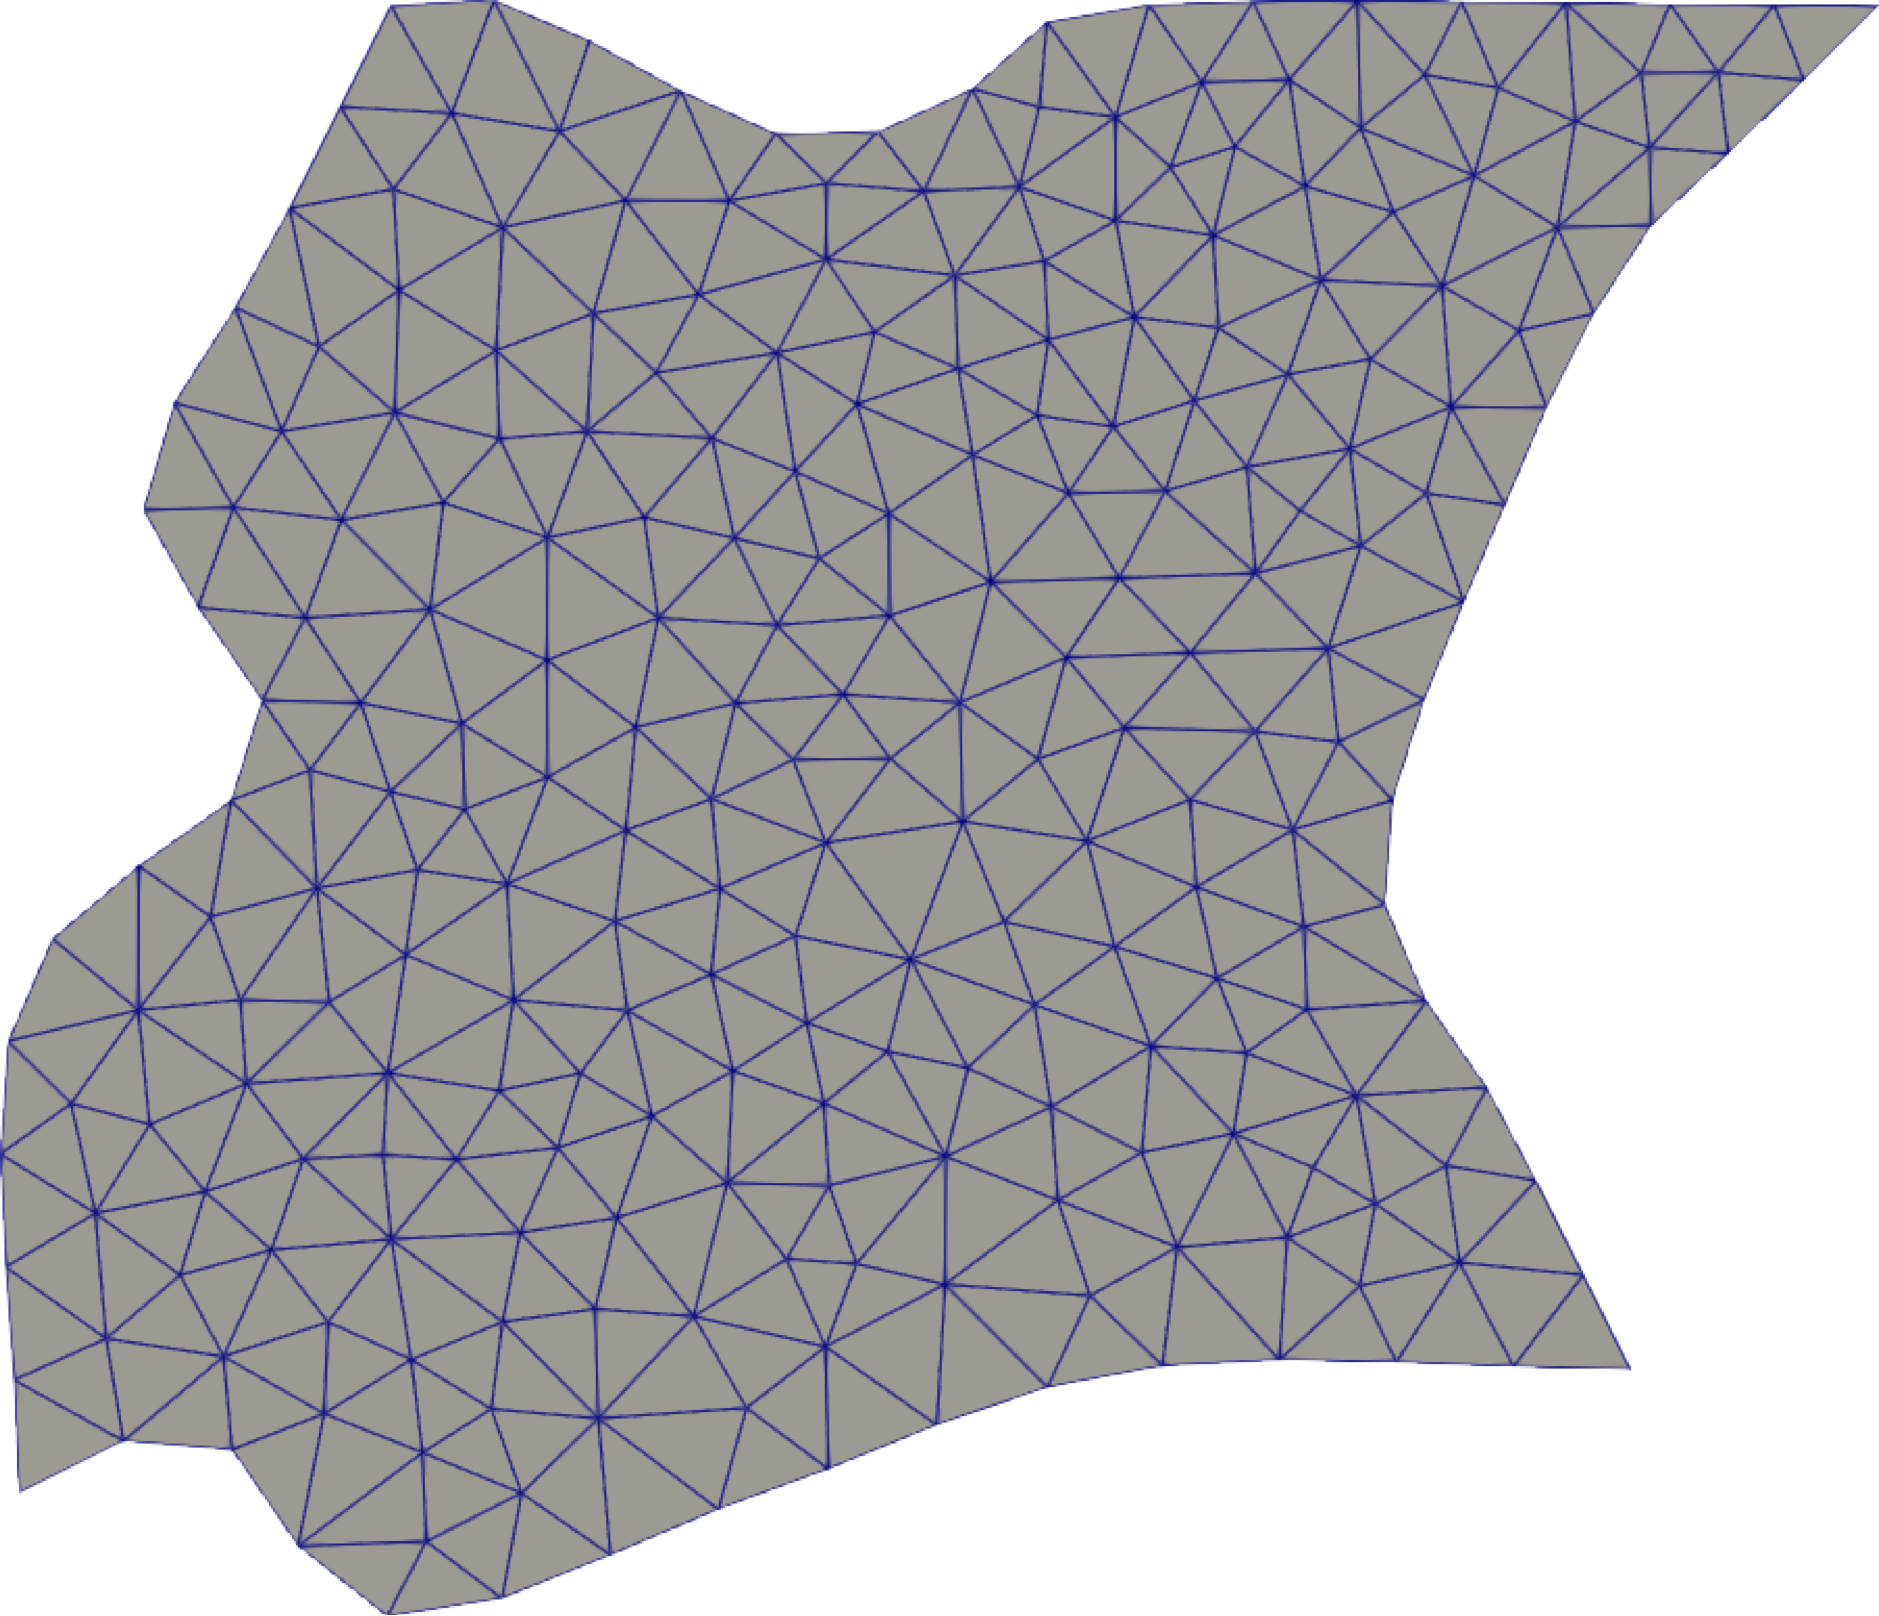
\includegraphics[scale=0.11]{images/zone4beamer.pdf}
        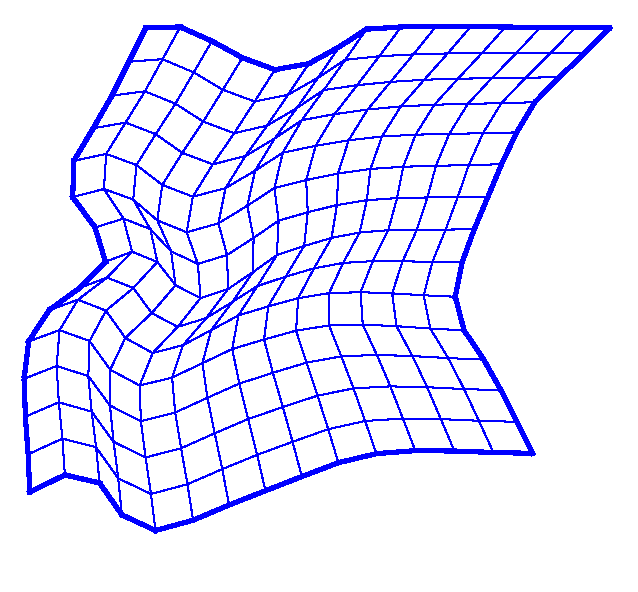
\includegraphics[scale=0.35]{images/mesh_zone4.eps}
    \end{column}
\end{columns}
\end{frame}

\begin{frame}
\frametitle{Contexte}
\small
\vspace{-0.2cm}
\begin{columns}
    \begin{column}{0.68\textwidth}
\textbf{Les caractéristiques recherchées pour les maillages quadrilatéraux.}\vspace{0.2cm}
\begin{itemize}

\onslide<1->{
\item {\color{onera} Structuré:} aspect régulier, stabilité.}
\vspace{0.1cm}

\onslide<2->{
\item {\color{onera} Fidélité géométrique:} mailles alignées le long du bord du domaine, conformité géométrique.}
\vspace{0.1cm}

\onslide<3->{
\item {\color{onera} Éléments de haute qualité:} mailles proches de carrés ou de rectangles, minimisation des risques de dégénérescence lors des transformations géométriques.}
\vspace{0.1cm}

\onslide<4->{
\item {\color{onera} Respect des contraintes de taille:} garantit la capture de variations locales, efficacité numérique globale.
}
\vspace{0.15cm}

\end{itemize}

\onslide<4->{
Le respect simultané de toutes ces contraintes rend difficile la génération automatique de maillages quadrilatéraux.}

    \end{column}

    \begin{column}{0.32\textwidth}
\centering
\only<1>{
\vspace{-0.15cm}
    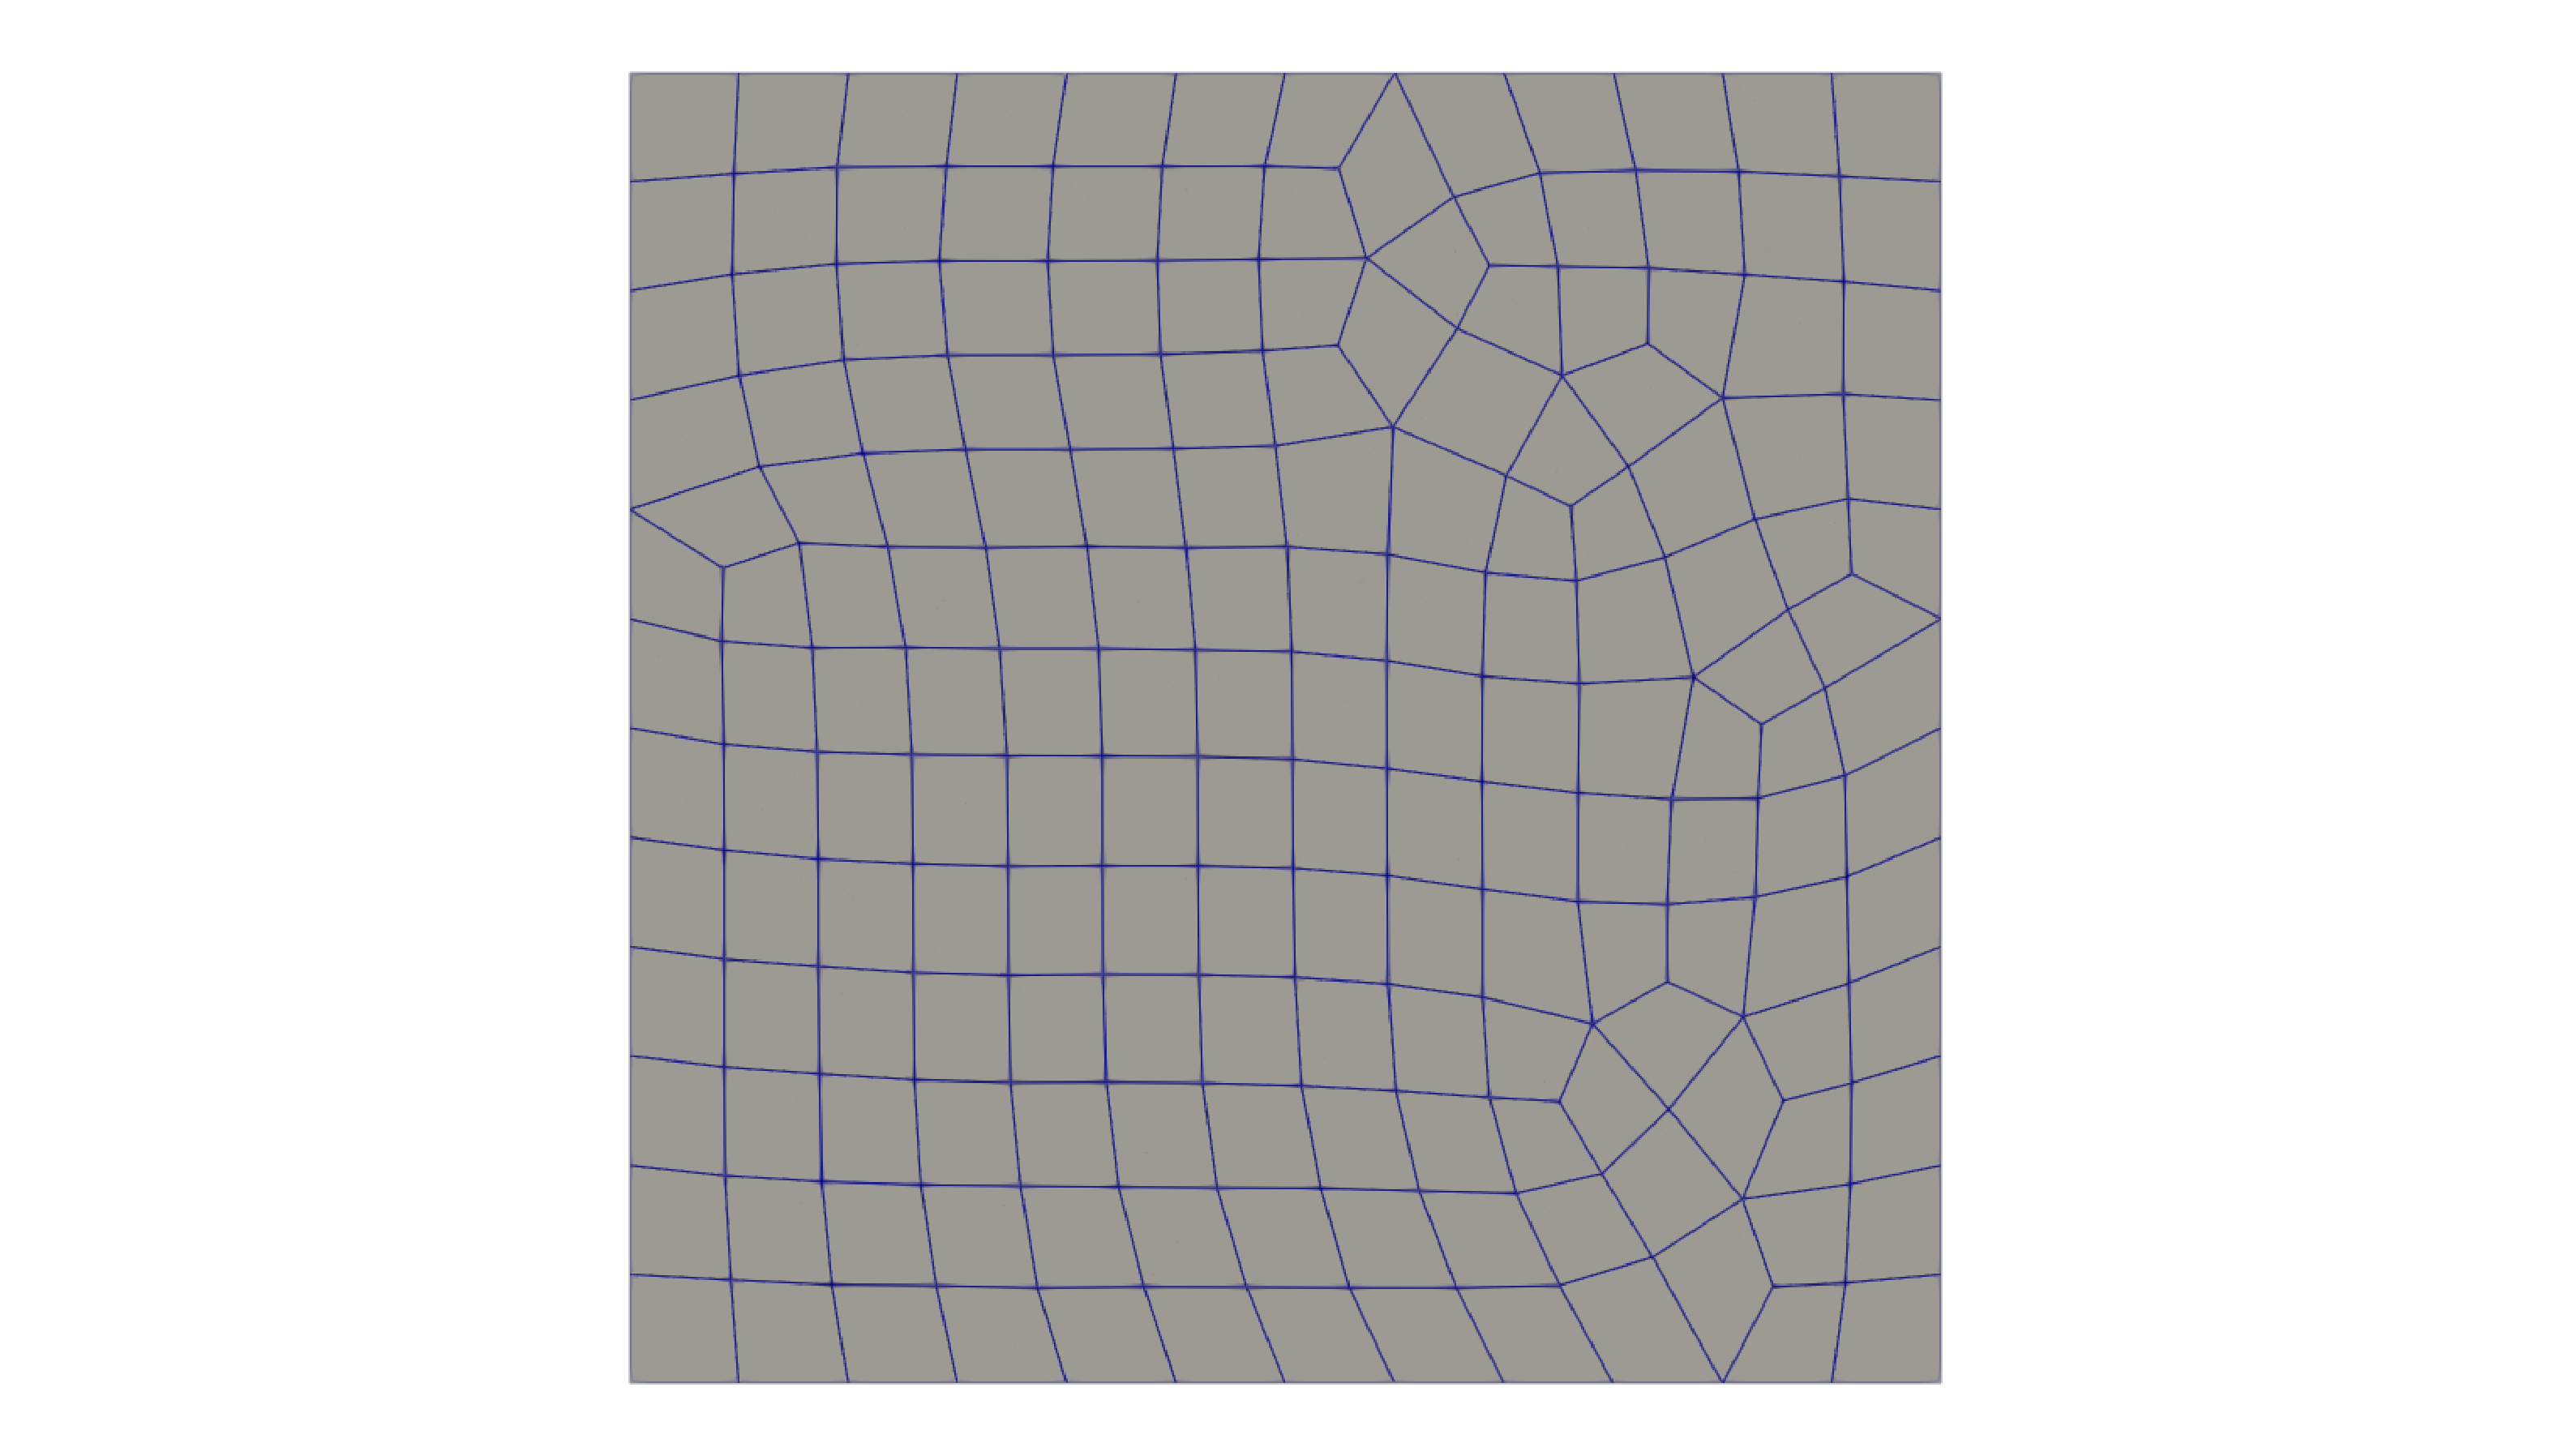
\includegraphics[scale=0.105]{images/irregularite_1.pdf}
    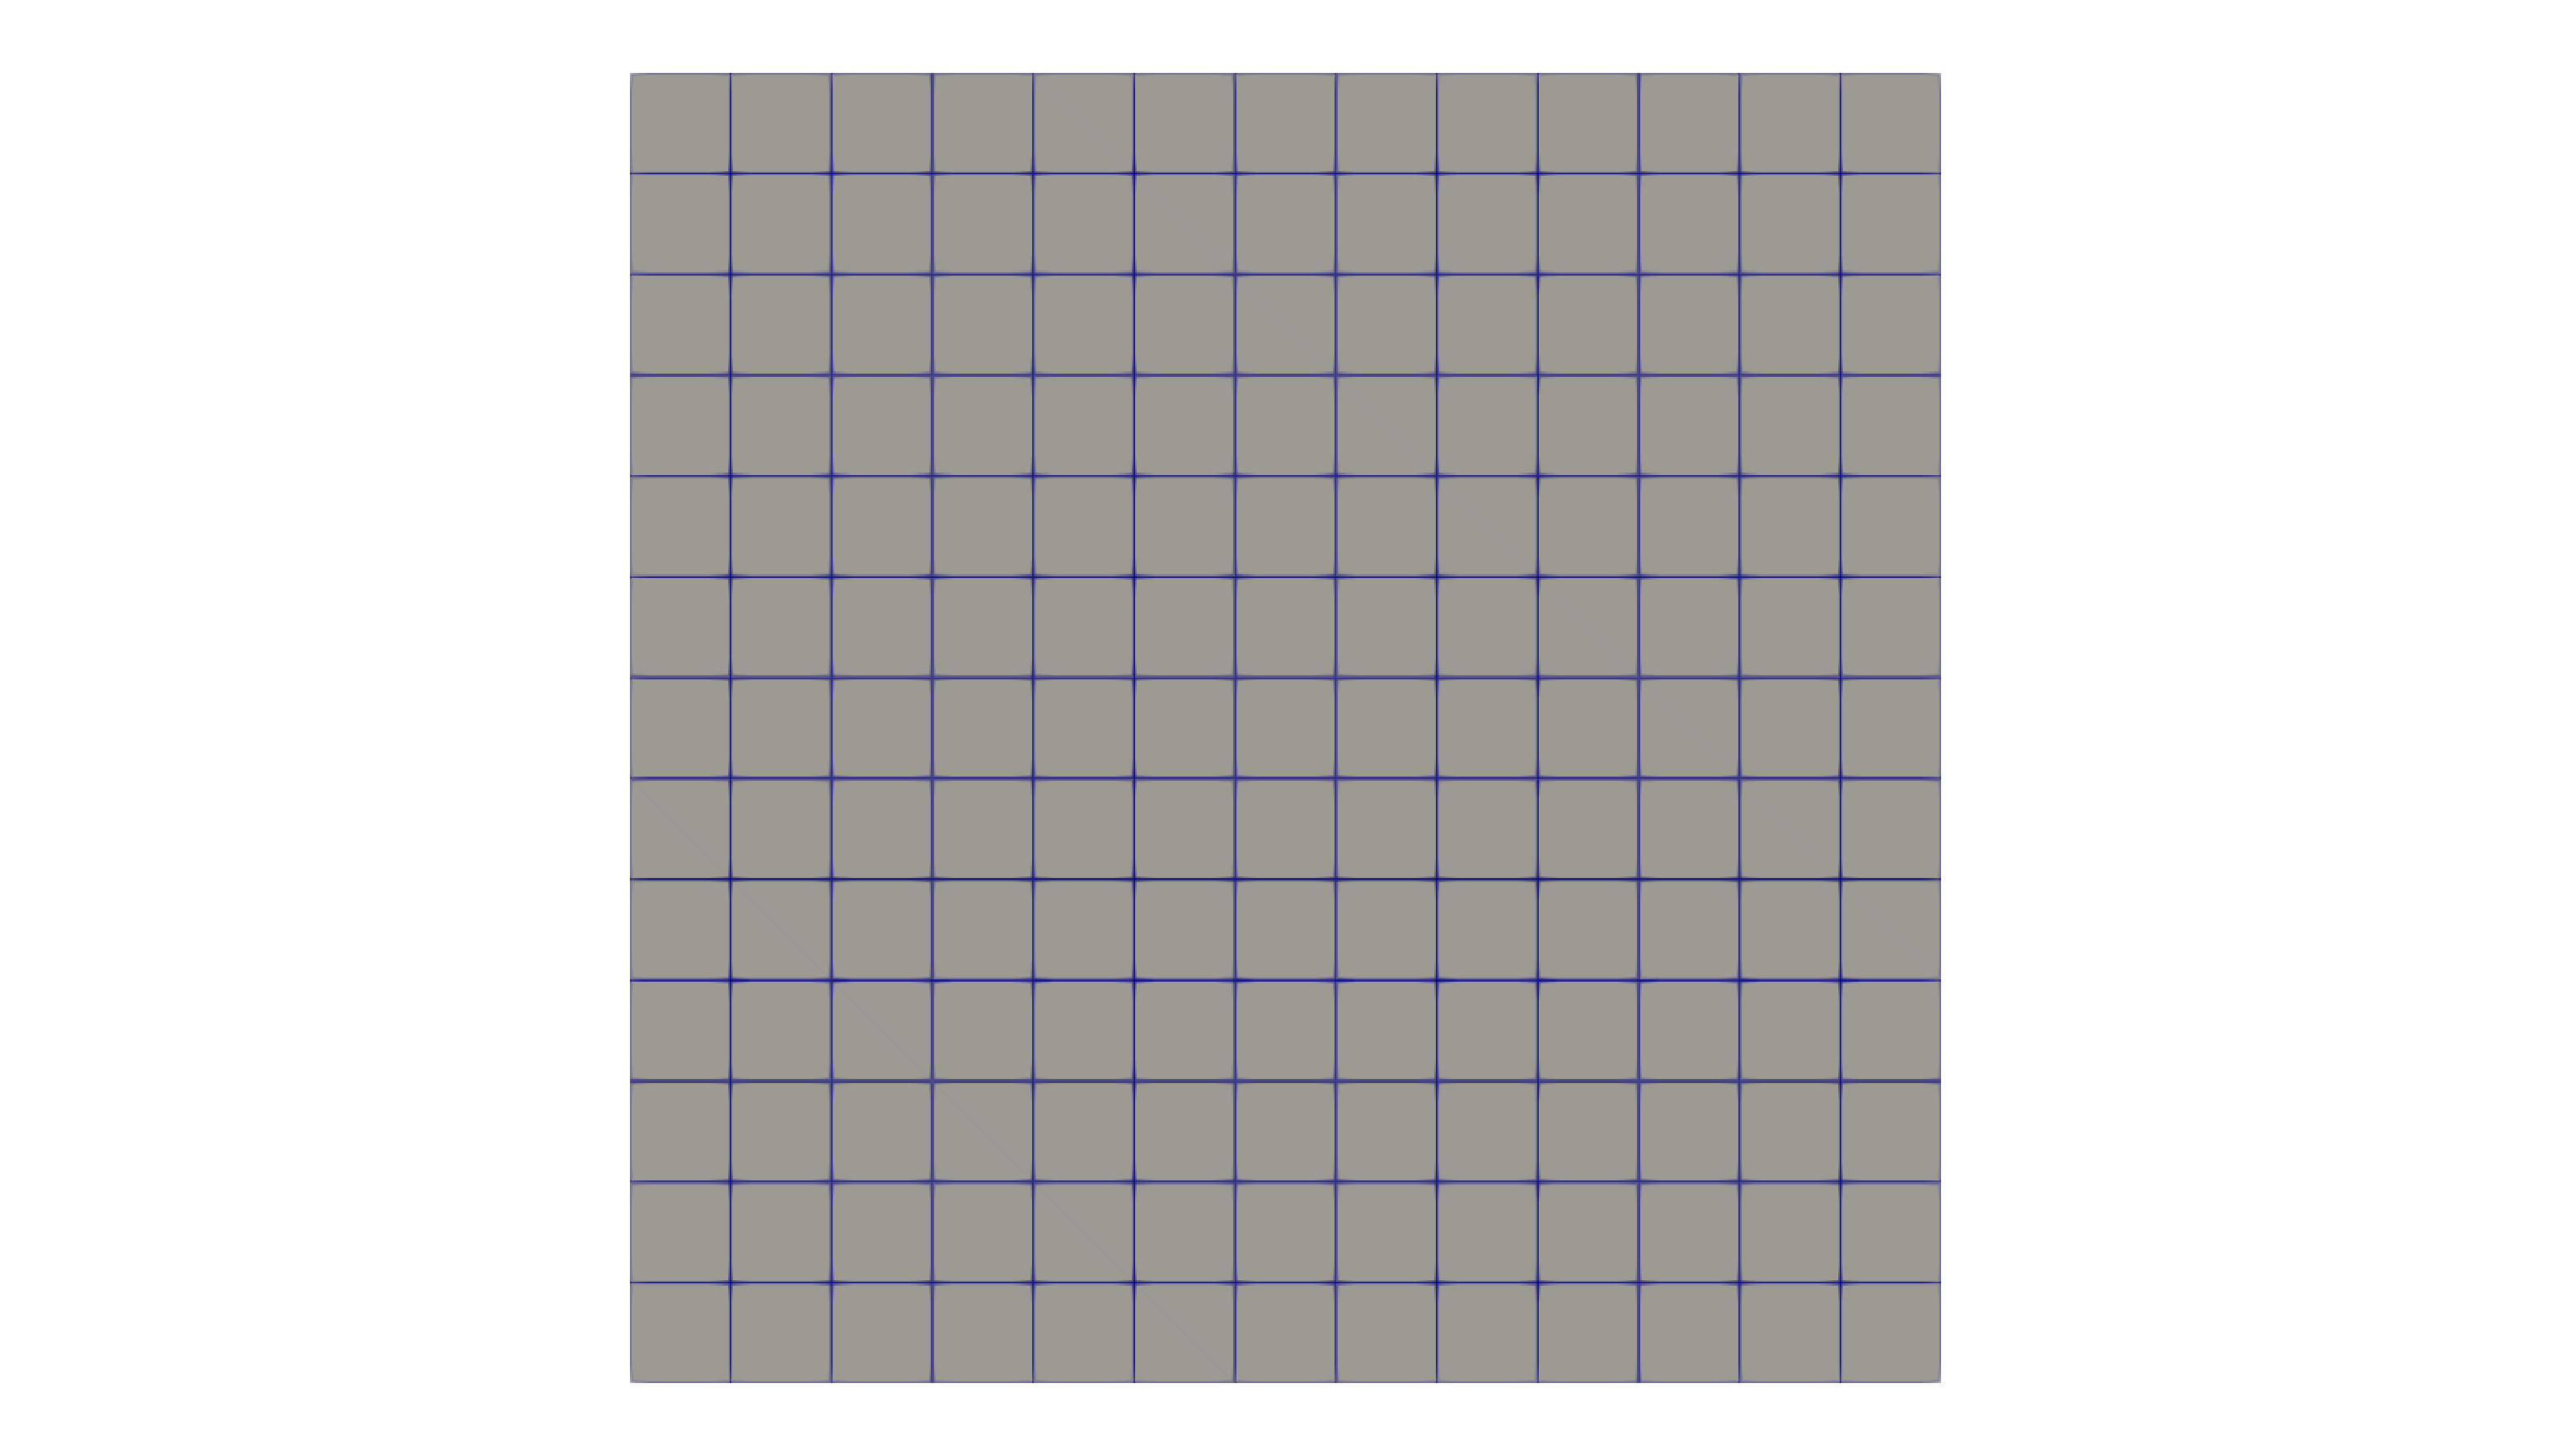
\includegraphics[scale=0.105]{images/irregularite_2.pdf}
\vspace{0.2cm}
}
\only<2>{
\centering
%\vspace{-0.2cm}
    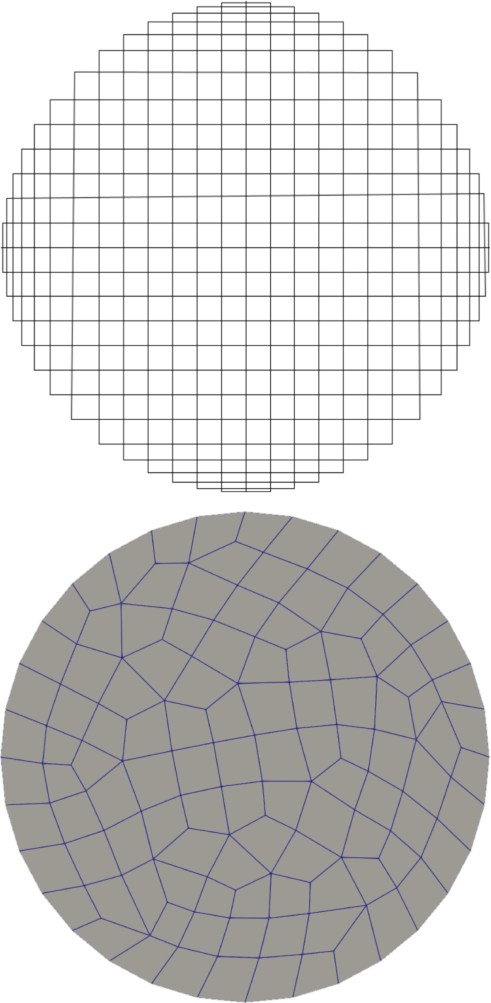
\includegraphics[scale=0.35]{images/align_bord.pdf}
\vspace{0.2cm}
}
\only<3>{
%\vspace{-0.2cm}
    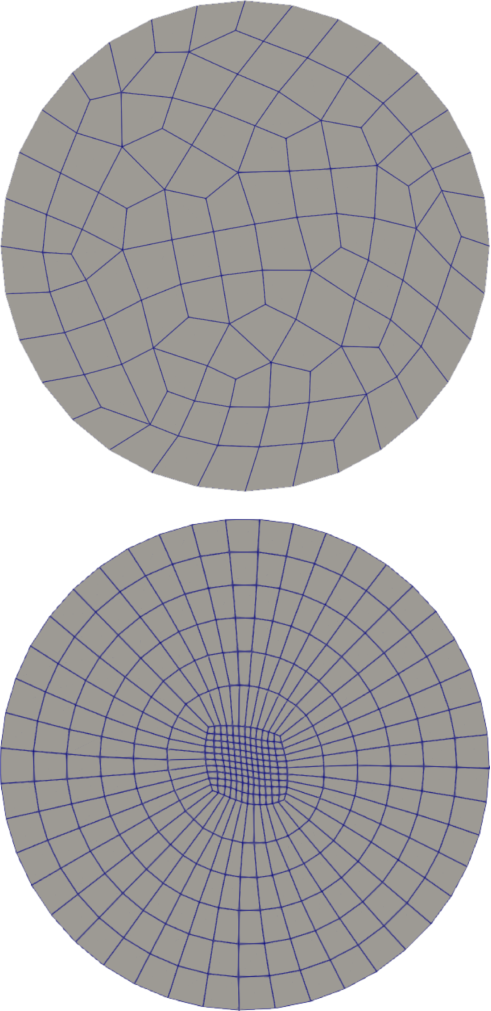
\includegraphics[scale=0.35]{images/element_quality.pdf}
\vspace{0.25cm}
}
\only<4>{
%\vspace{-0.2cm}
    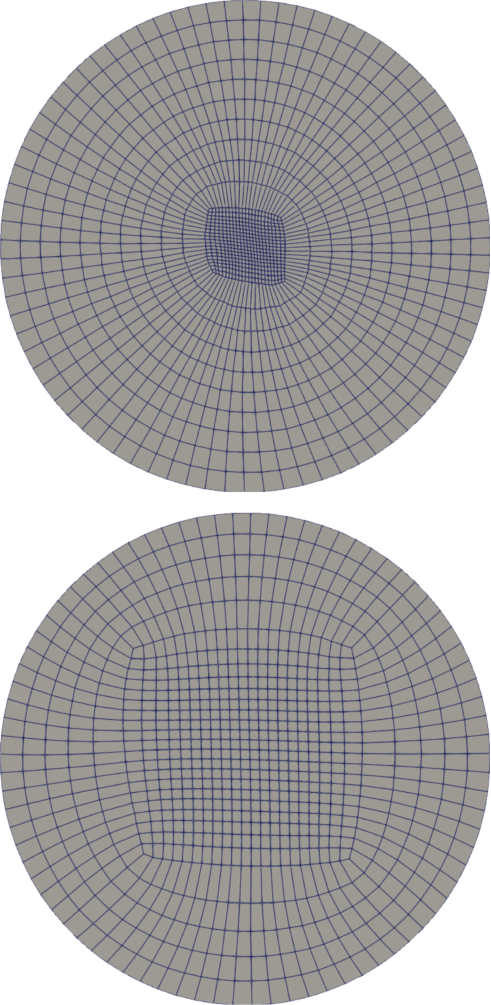
\includegraphics[scale=0.35]{images/explosion.pdf}
\vspace{0.25cm}
}
\end{column}
\end{columns}
\end{frame}


\begin{frame}
\frametitle{Contexte}
%\small
\begin{columns}
    \begin{column}{0.68\textwidth}
        {\bf Quelques méthodes de génération de "Mesh quad".}\vspace{0.2cm}
        \begin{itemize}


\onslide<1->{
            \item {\color{onera} Blocs structurés manuels}\\\vspace{0.1cm}}

\onslide<2->{
            \item {\color{onera} Conversion Tri-to-quad:} subdivision de Catmull-Clark {\color{gray} [ E. Catmull, J. Clark (1978)]}, operation edge-flip {\color{onera_gray} [ MeshLab, SQuad, BlossomQuad (2011)]}, quads non-structuré.}\\\vspace{0.1cm}


\onslide<3->{
            \item {\color{onera} Méthodes de grille cartésienne:} intersection domaine-grille {\color{onera_gray} [Schneiders (1996)]}, génèrent des mailles de mauvaises qualités le long de la frontière}\\\vspace{0.1cm}


\onslide<4->{
            \item {\color{onera} Avancée de front:} pavage {\color{onera_gray}[D. Blacker, B. Stephenson (1991)]}, H-Morph {\color{onera_gray}[Owen et al (2000)]}.}\vspace{0.1cm}


%\onslide<5->{\item {\color{onera} Axe médian:} simplification de la géomtrie en identifiant un squelette central {\color{onera_gray}[Nackman and Srinivasan, 1989]}.}\vspace{0.1cm}

        \end{itemize}
    \end{column}


        \begin{column}{0.4\textwidth}
\centering
\only<2>{
\vspace{-0.15cm}
    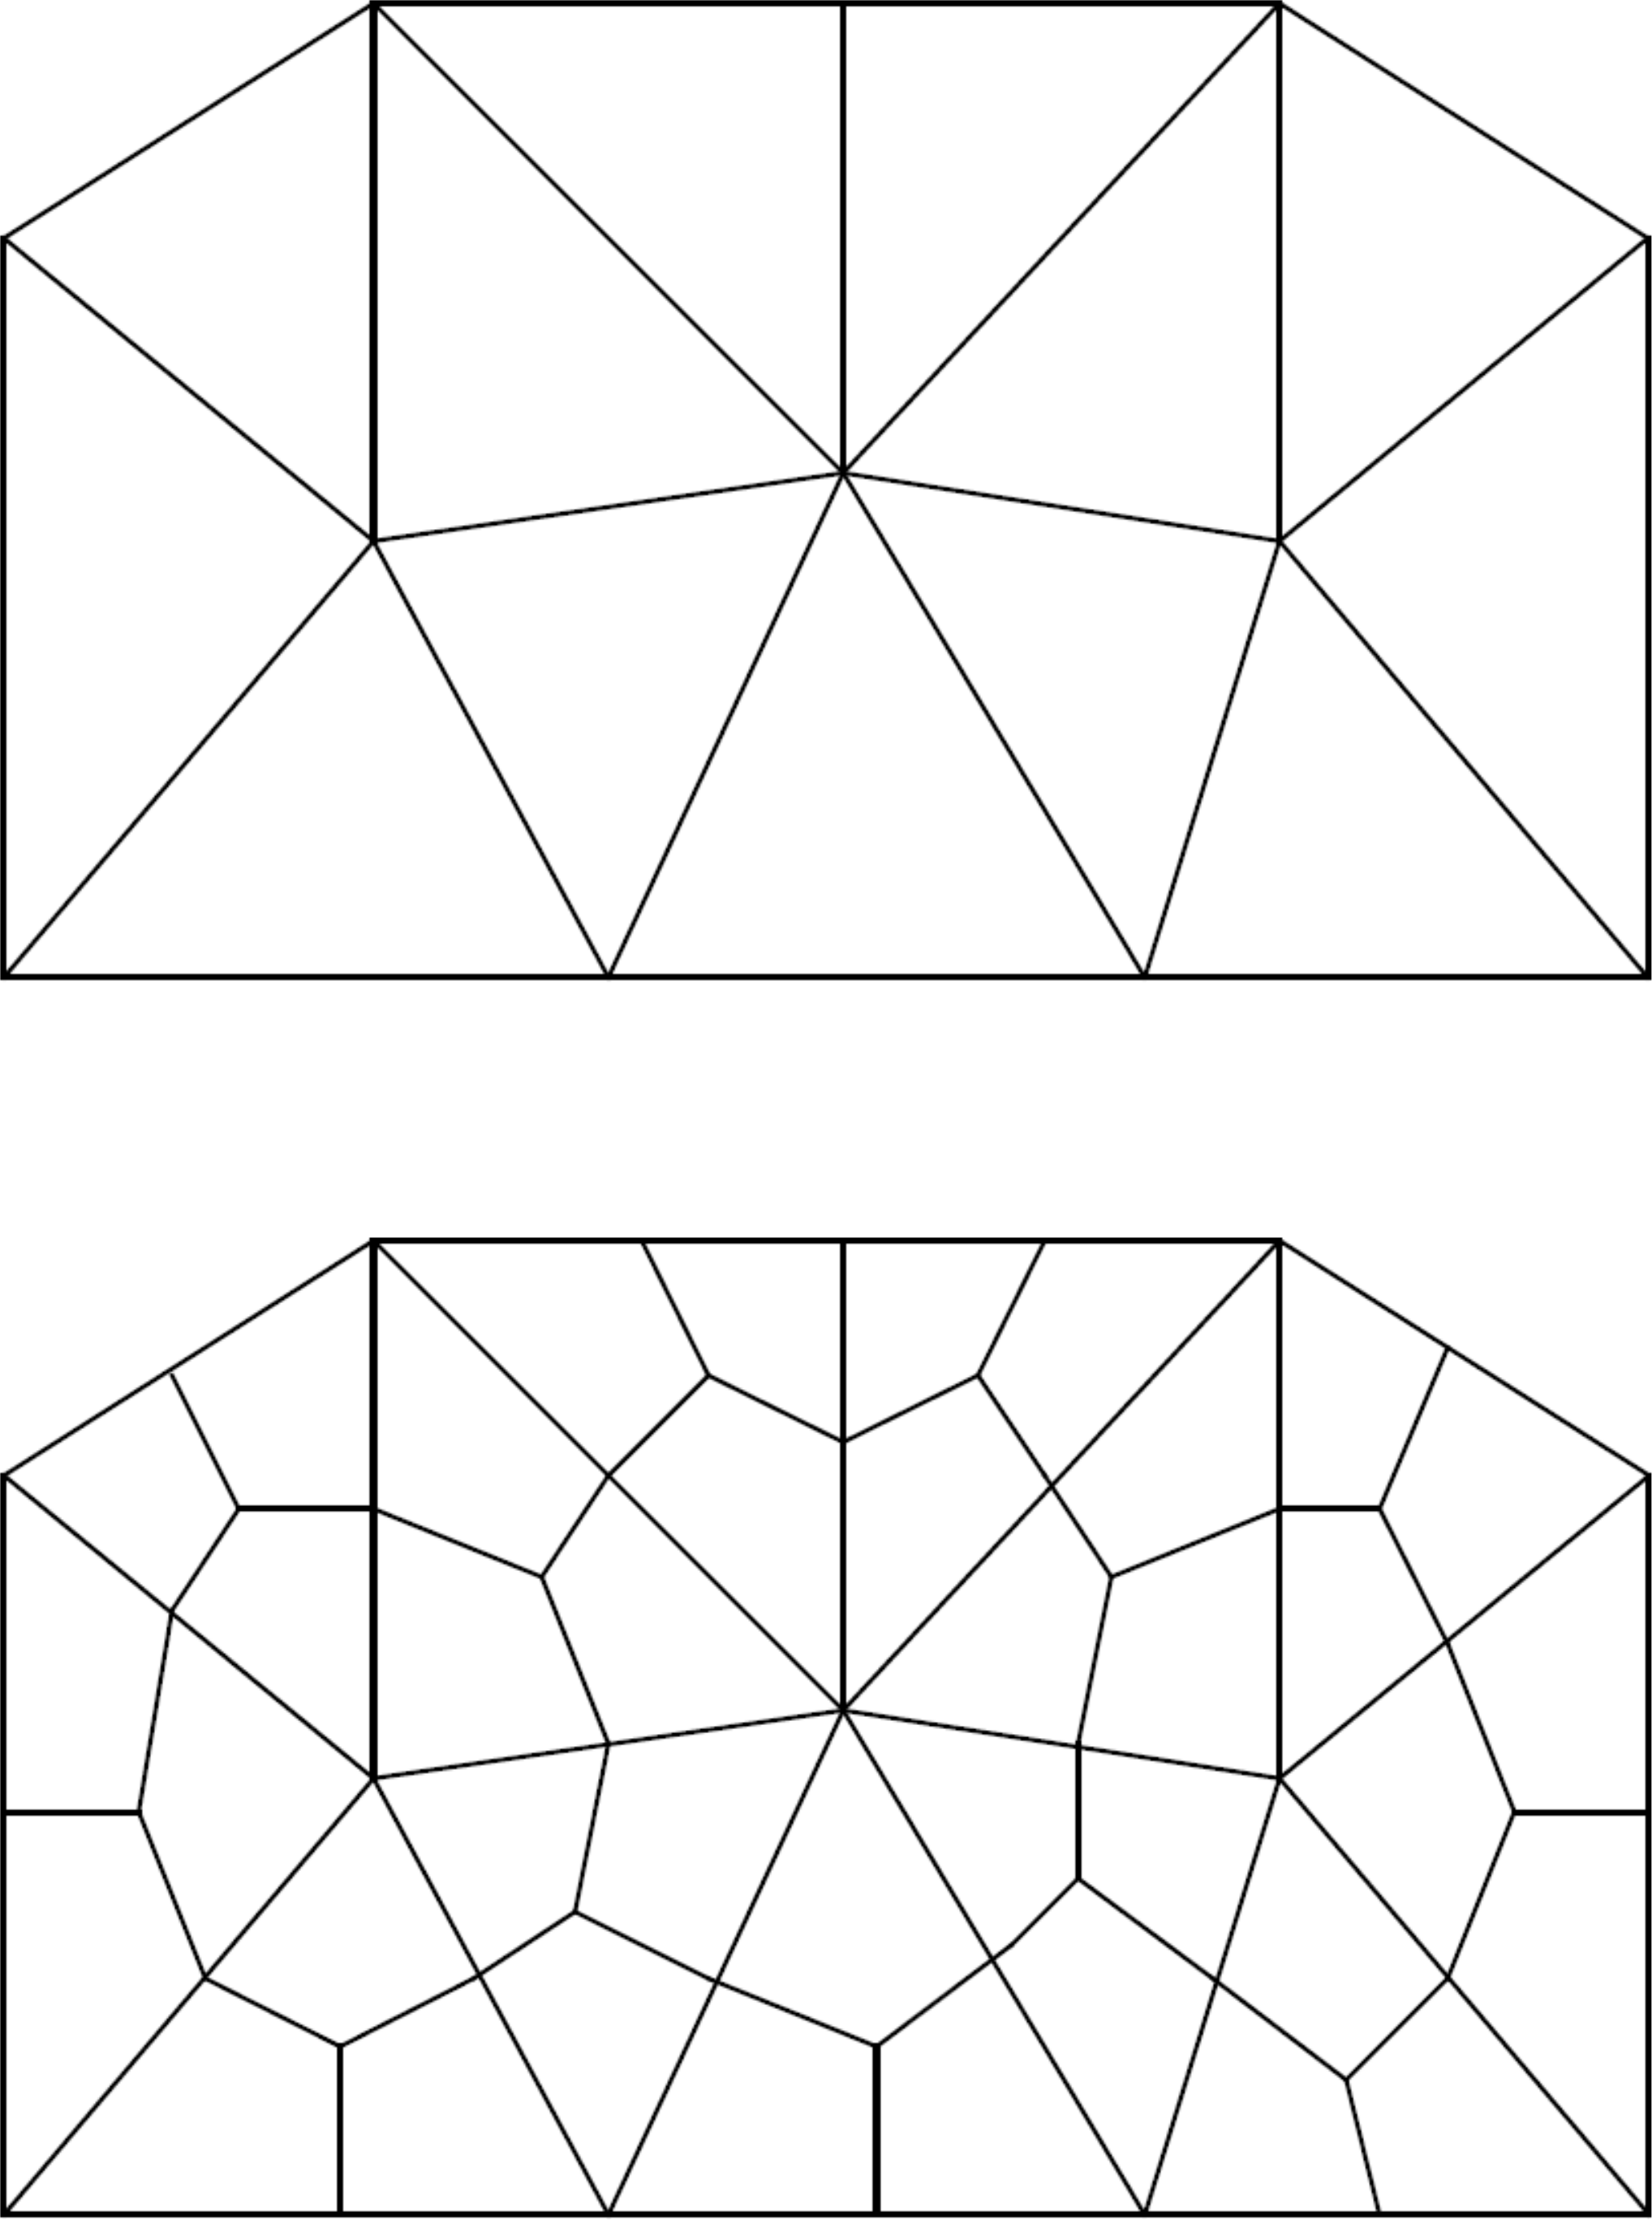
\includegraphics[scale=0.22]{images/tri_to_quad_1_beam.png}
\vspace{0.2cm}
}
\only<3>{
%\vspace{-0.2cm}
    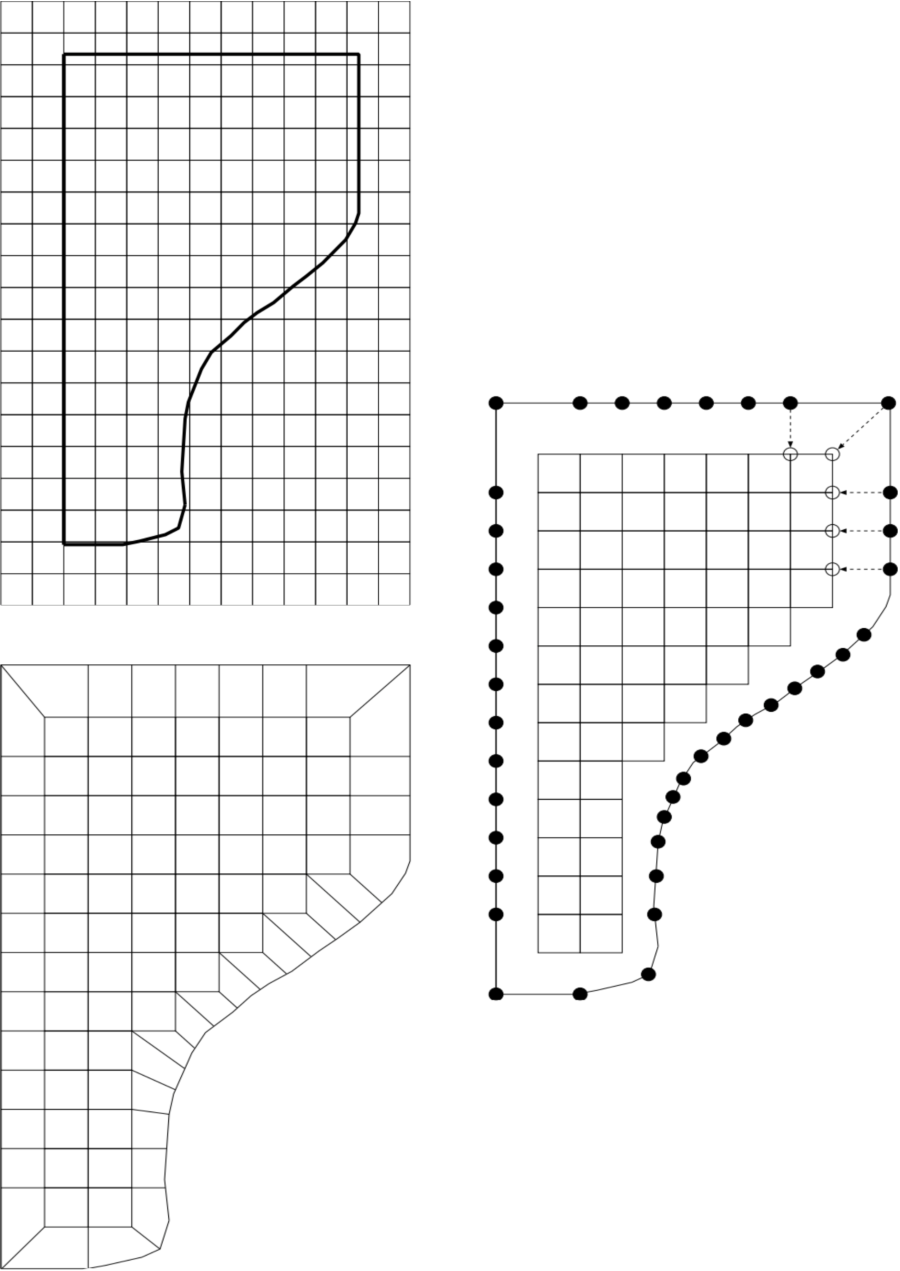
\includegraphics[scale=0.28]{images/superpo_grid_1_beam.pdf}
\vspace{0.18cm}
}
\only<4>{
%\vspace{-0.2cm}
    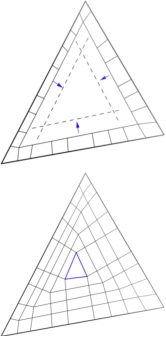
\includegraphics[scale=1]{images/front_advance_beam.pdf}
%\vspace{0.15cm}
}
%\only<4>{
%\vspace{-0.2cm}
    %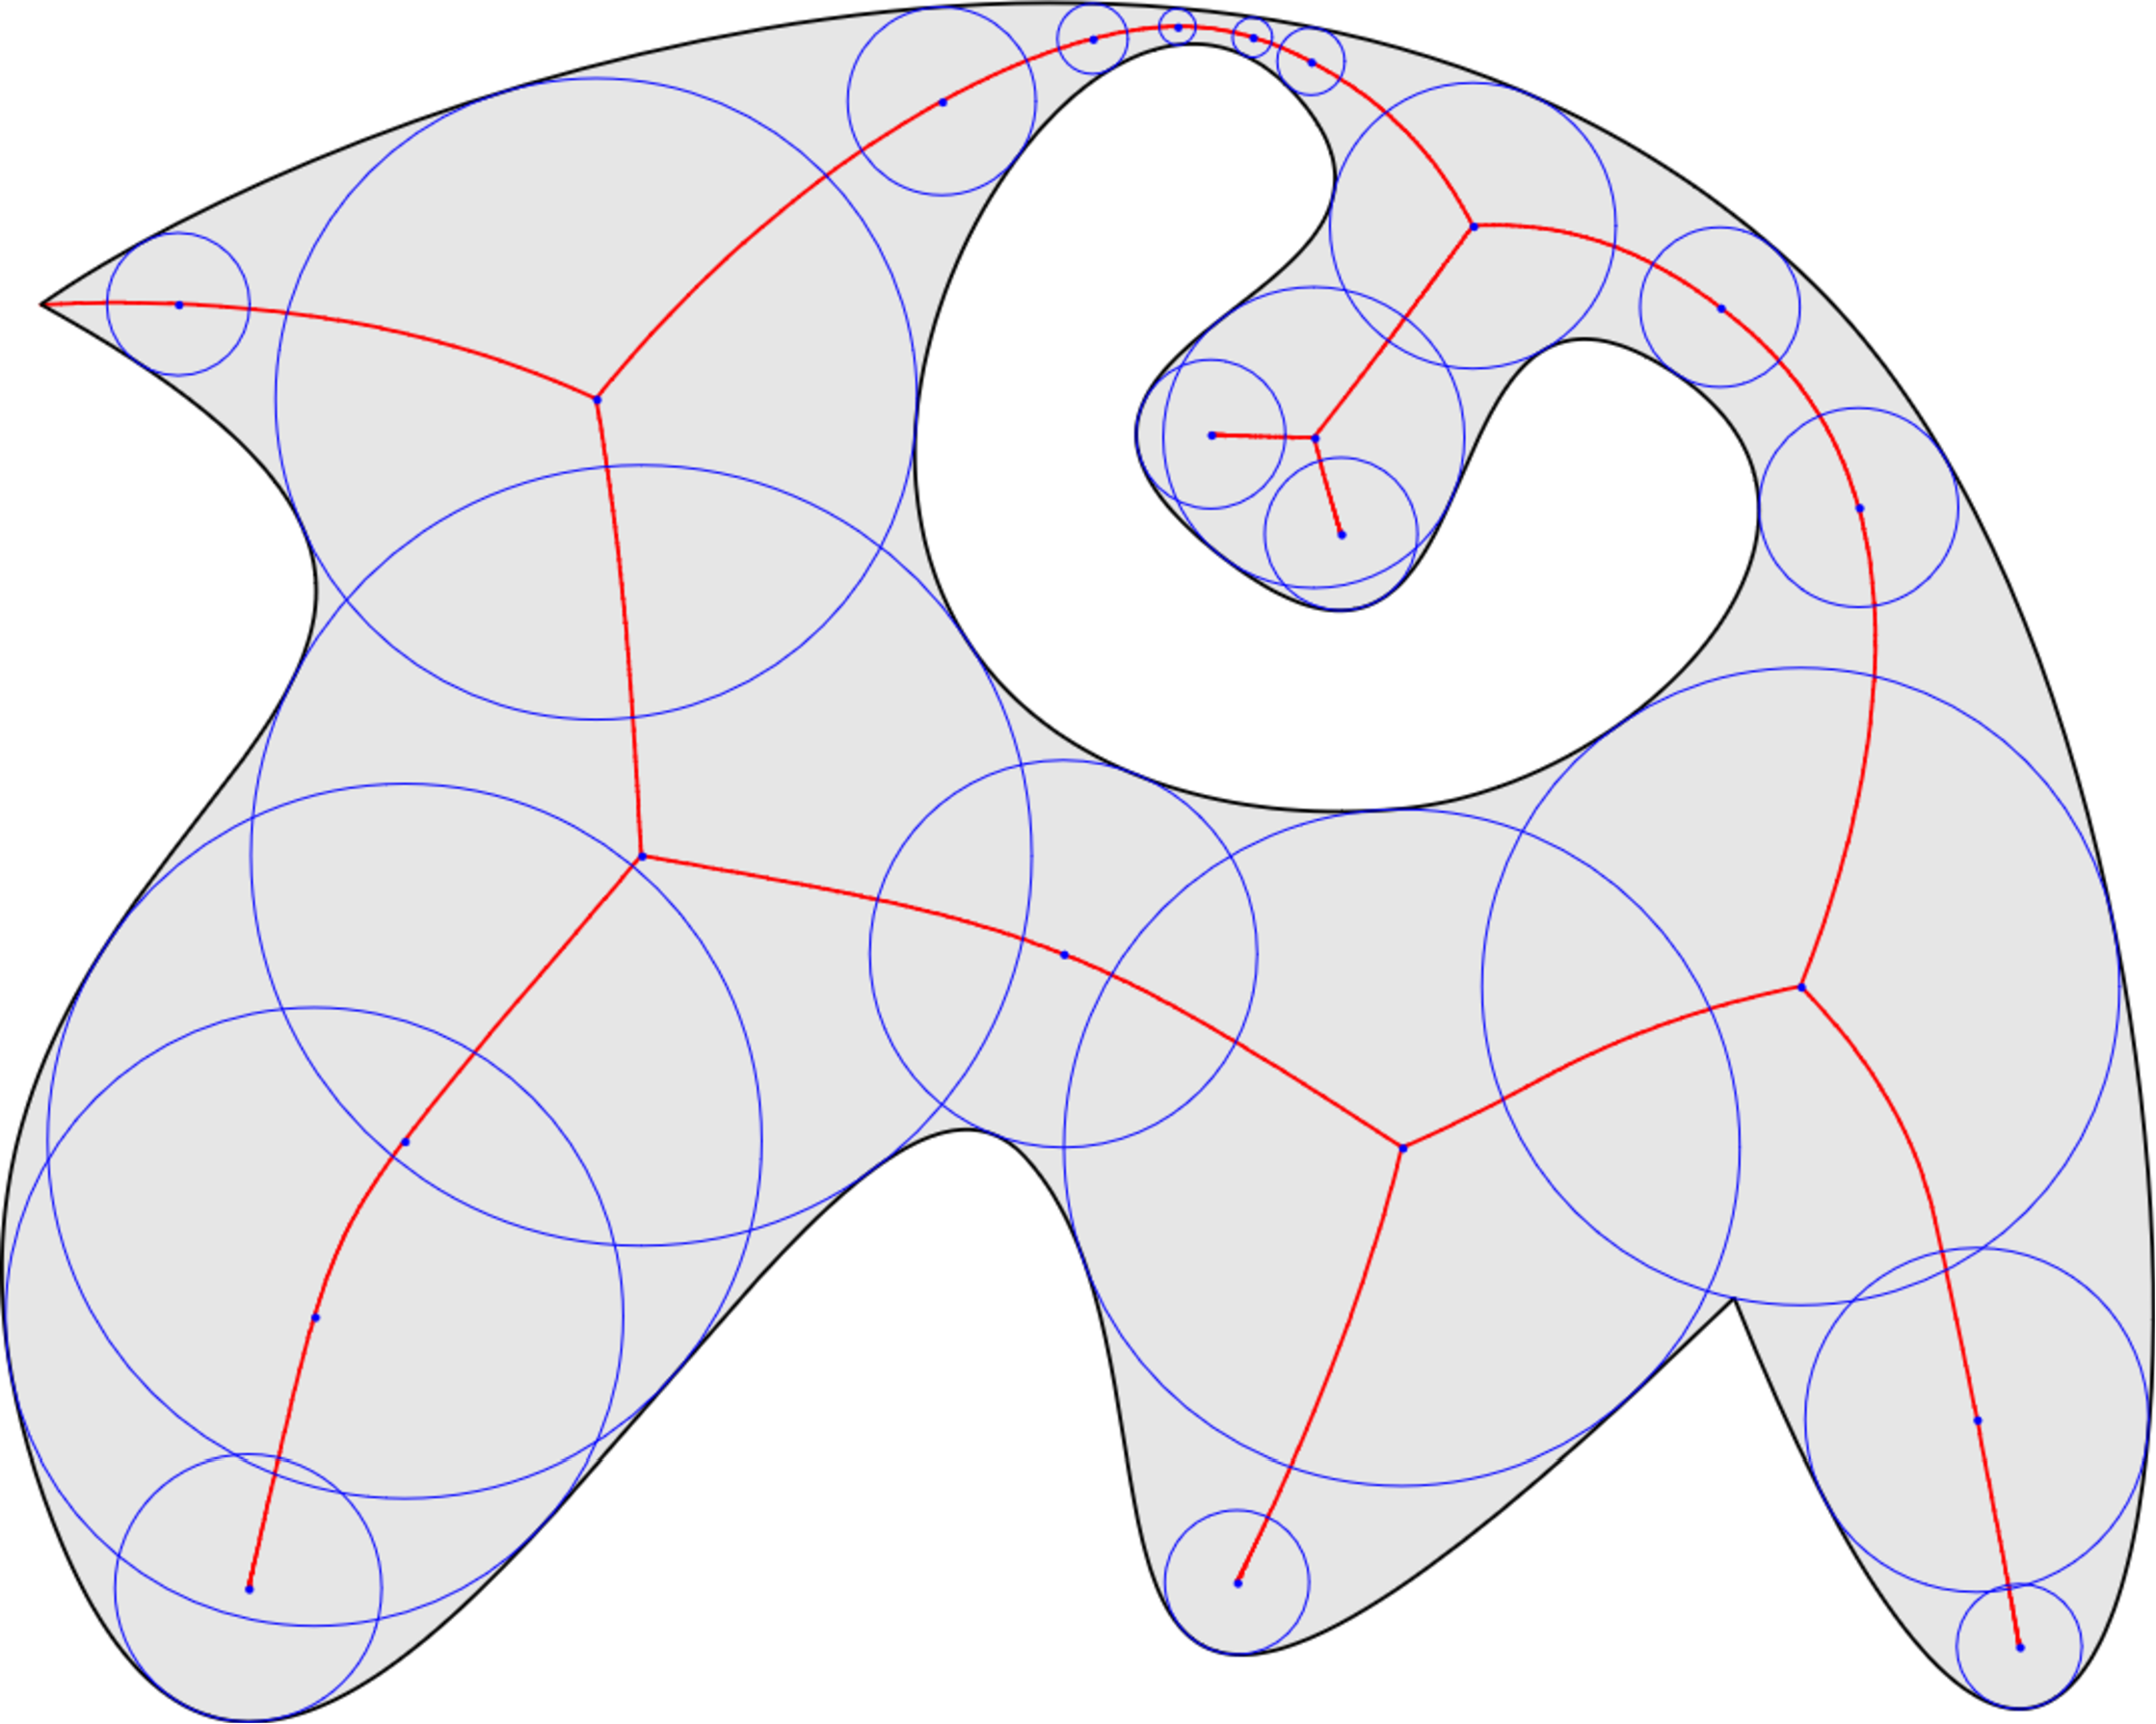
\includegraphics[scale=0.13]{images/median_axis.pdf}
%\vspace{0.15cm}
%}
\end{column}
\end{columns}
\end{frame}



\begin{frame}{Une approche basée sur les champs de croix}
\begin{columns}

\begin{column}{0.25\textwidth}
\centering
\onslide<1->{
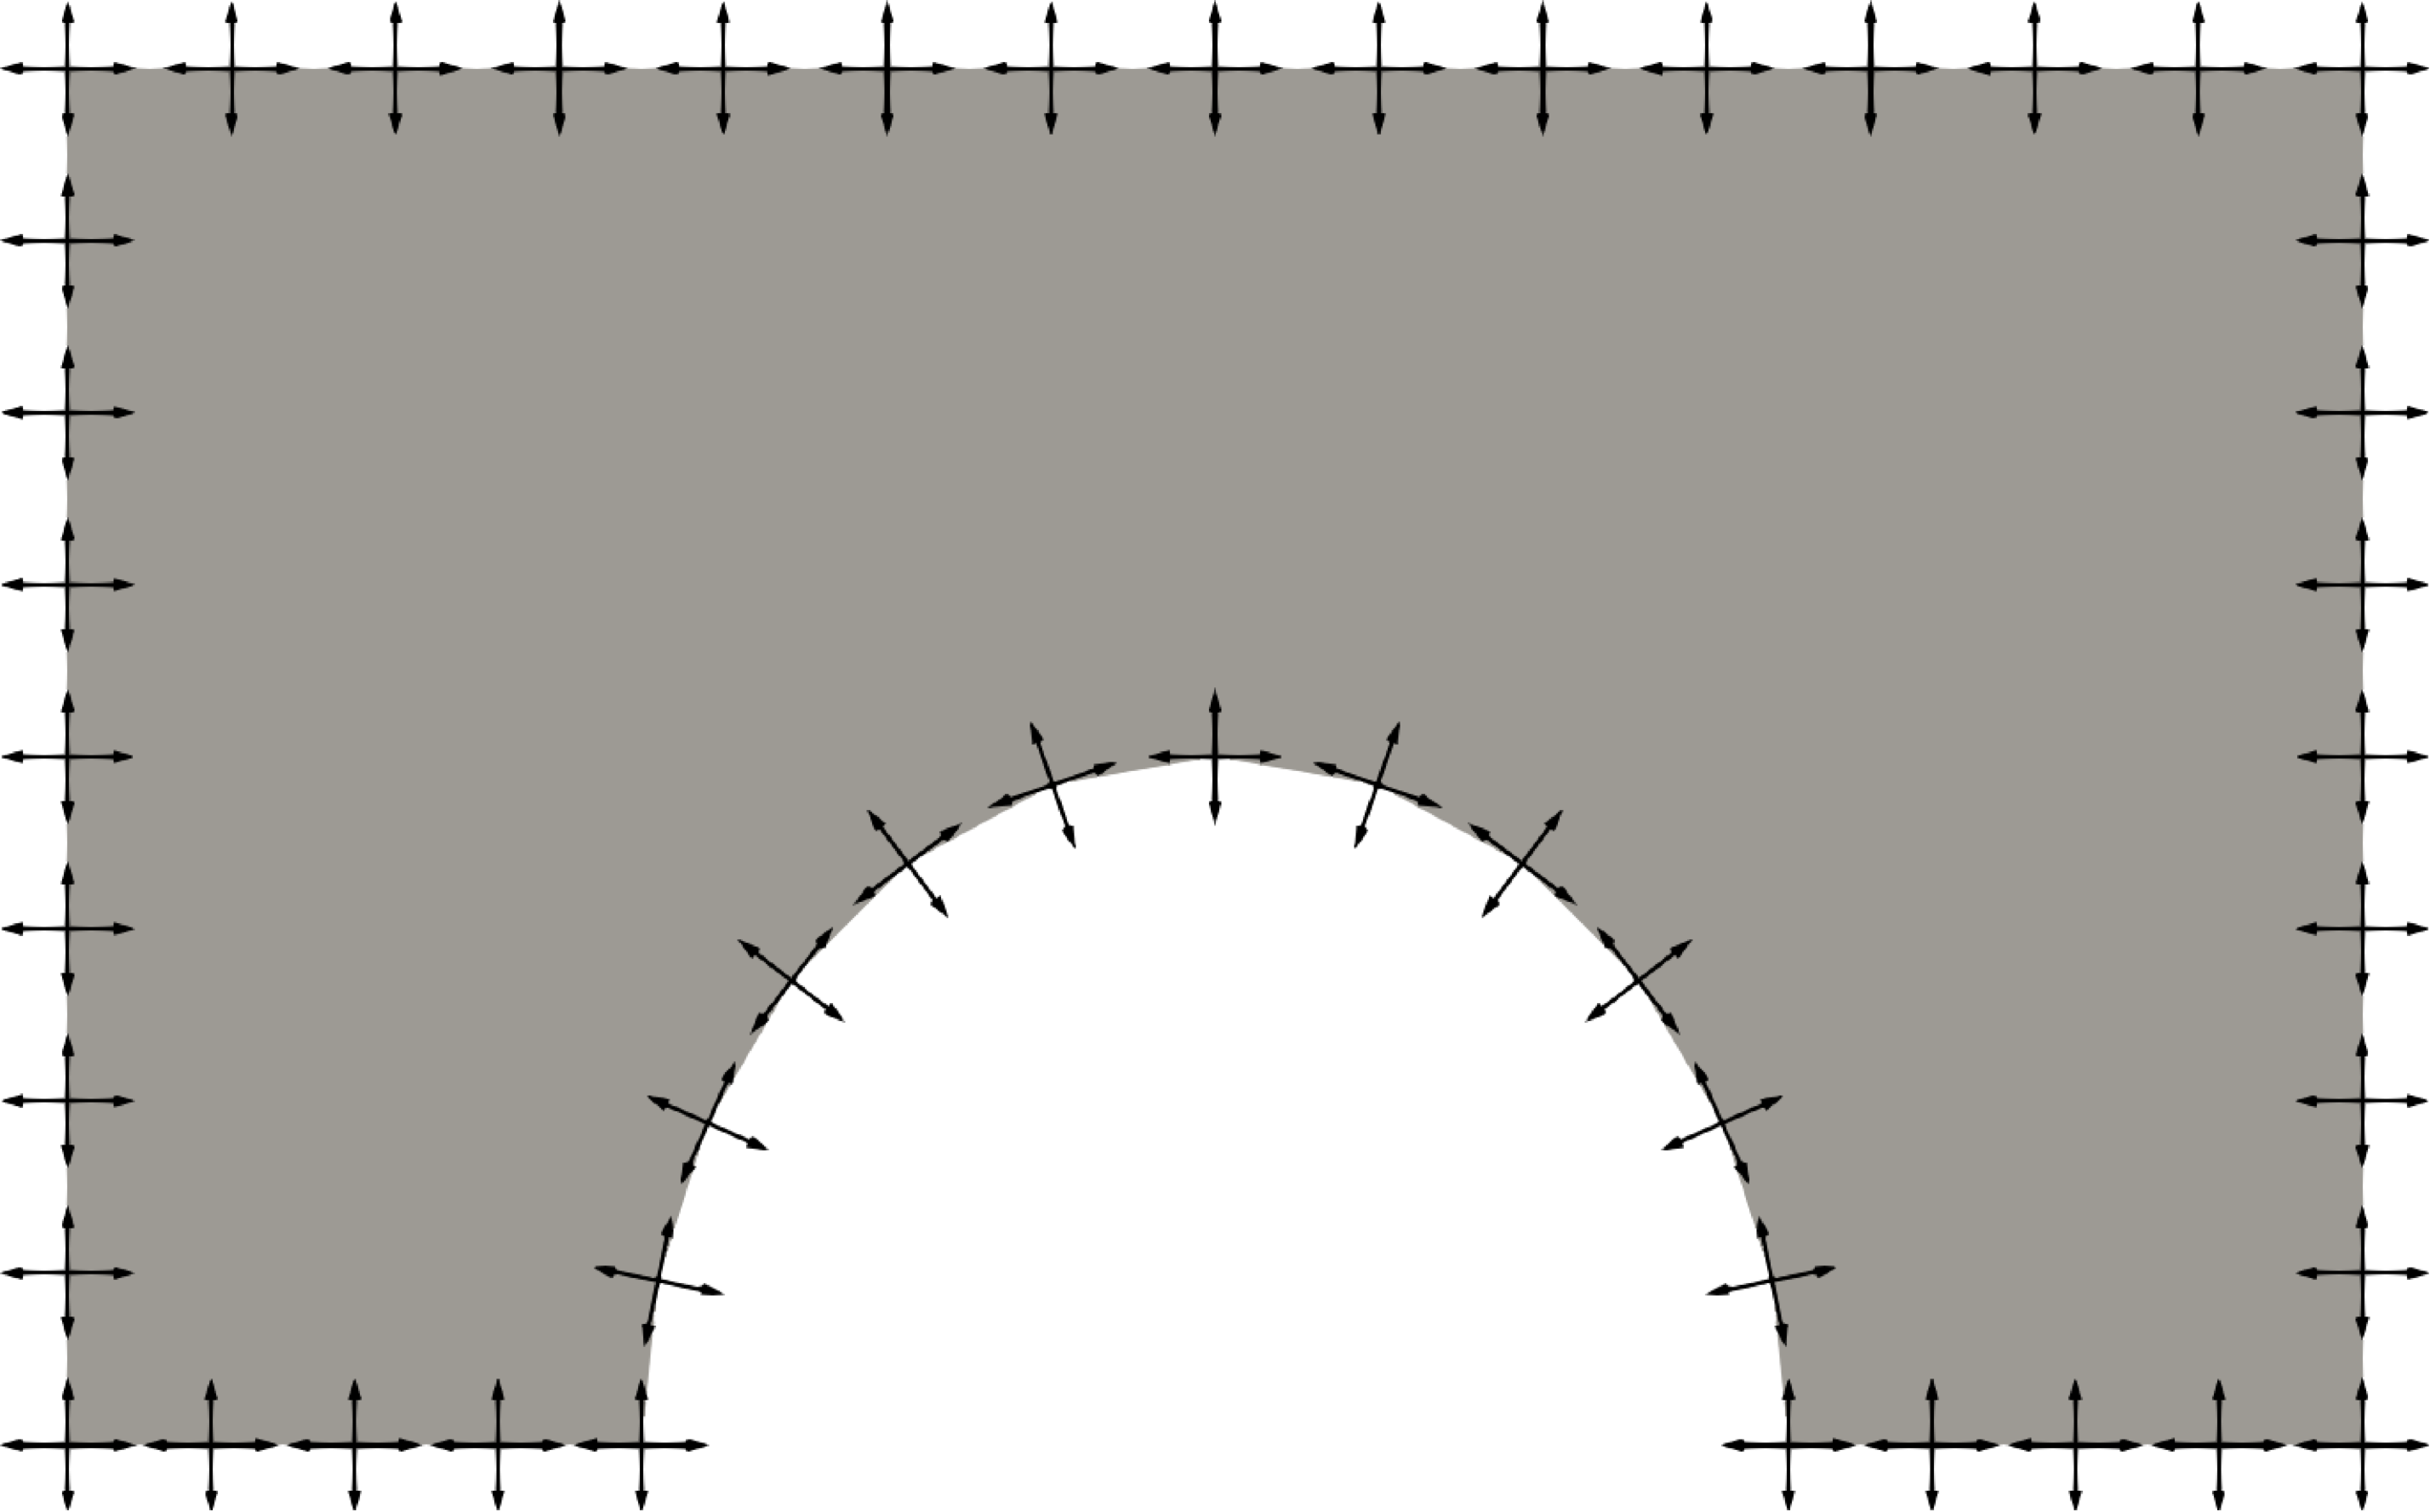
\includegraphics[scale=0.068]{images/frey_1.pdf}\hspace{0.2cm}
\footnotesize Croix de bord
%}
\end{column}

\begin{column}{0.25\textwidth}
\centering
%\onslide<2->{
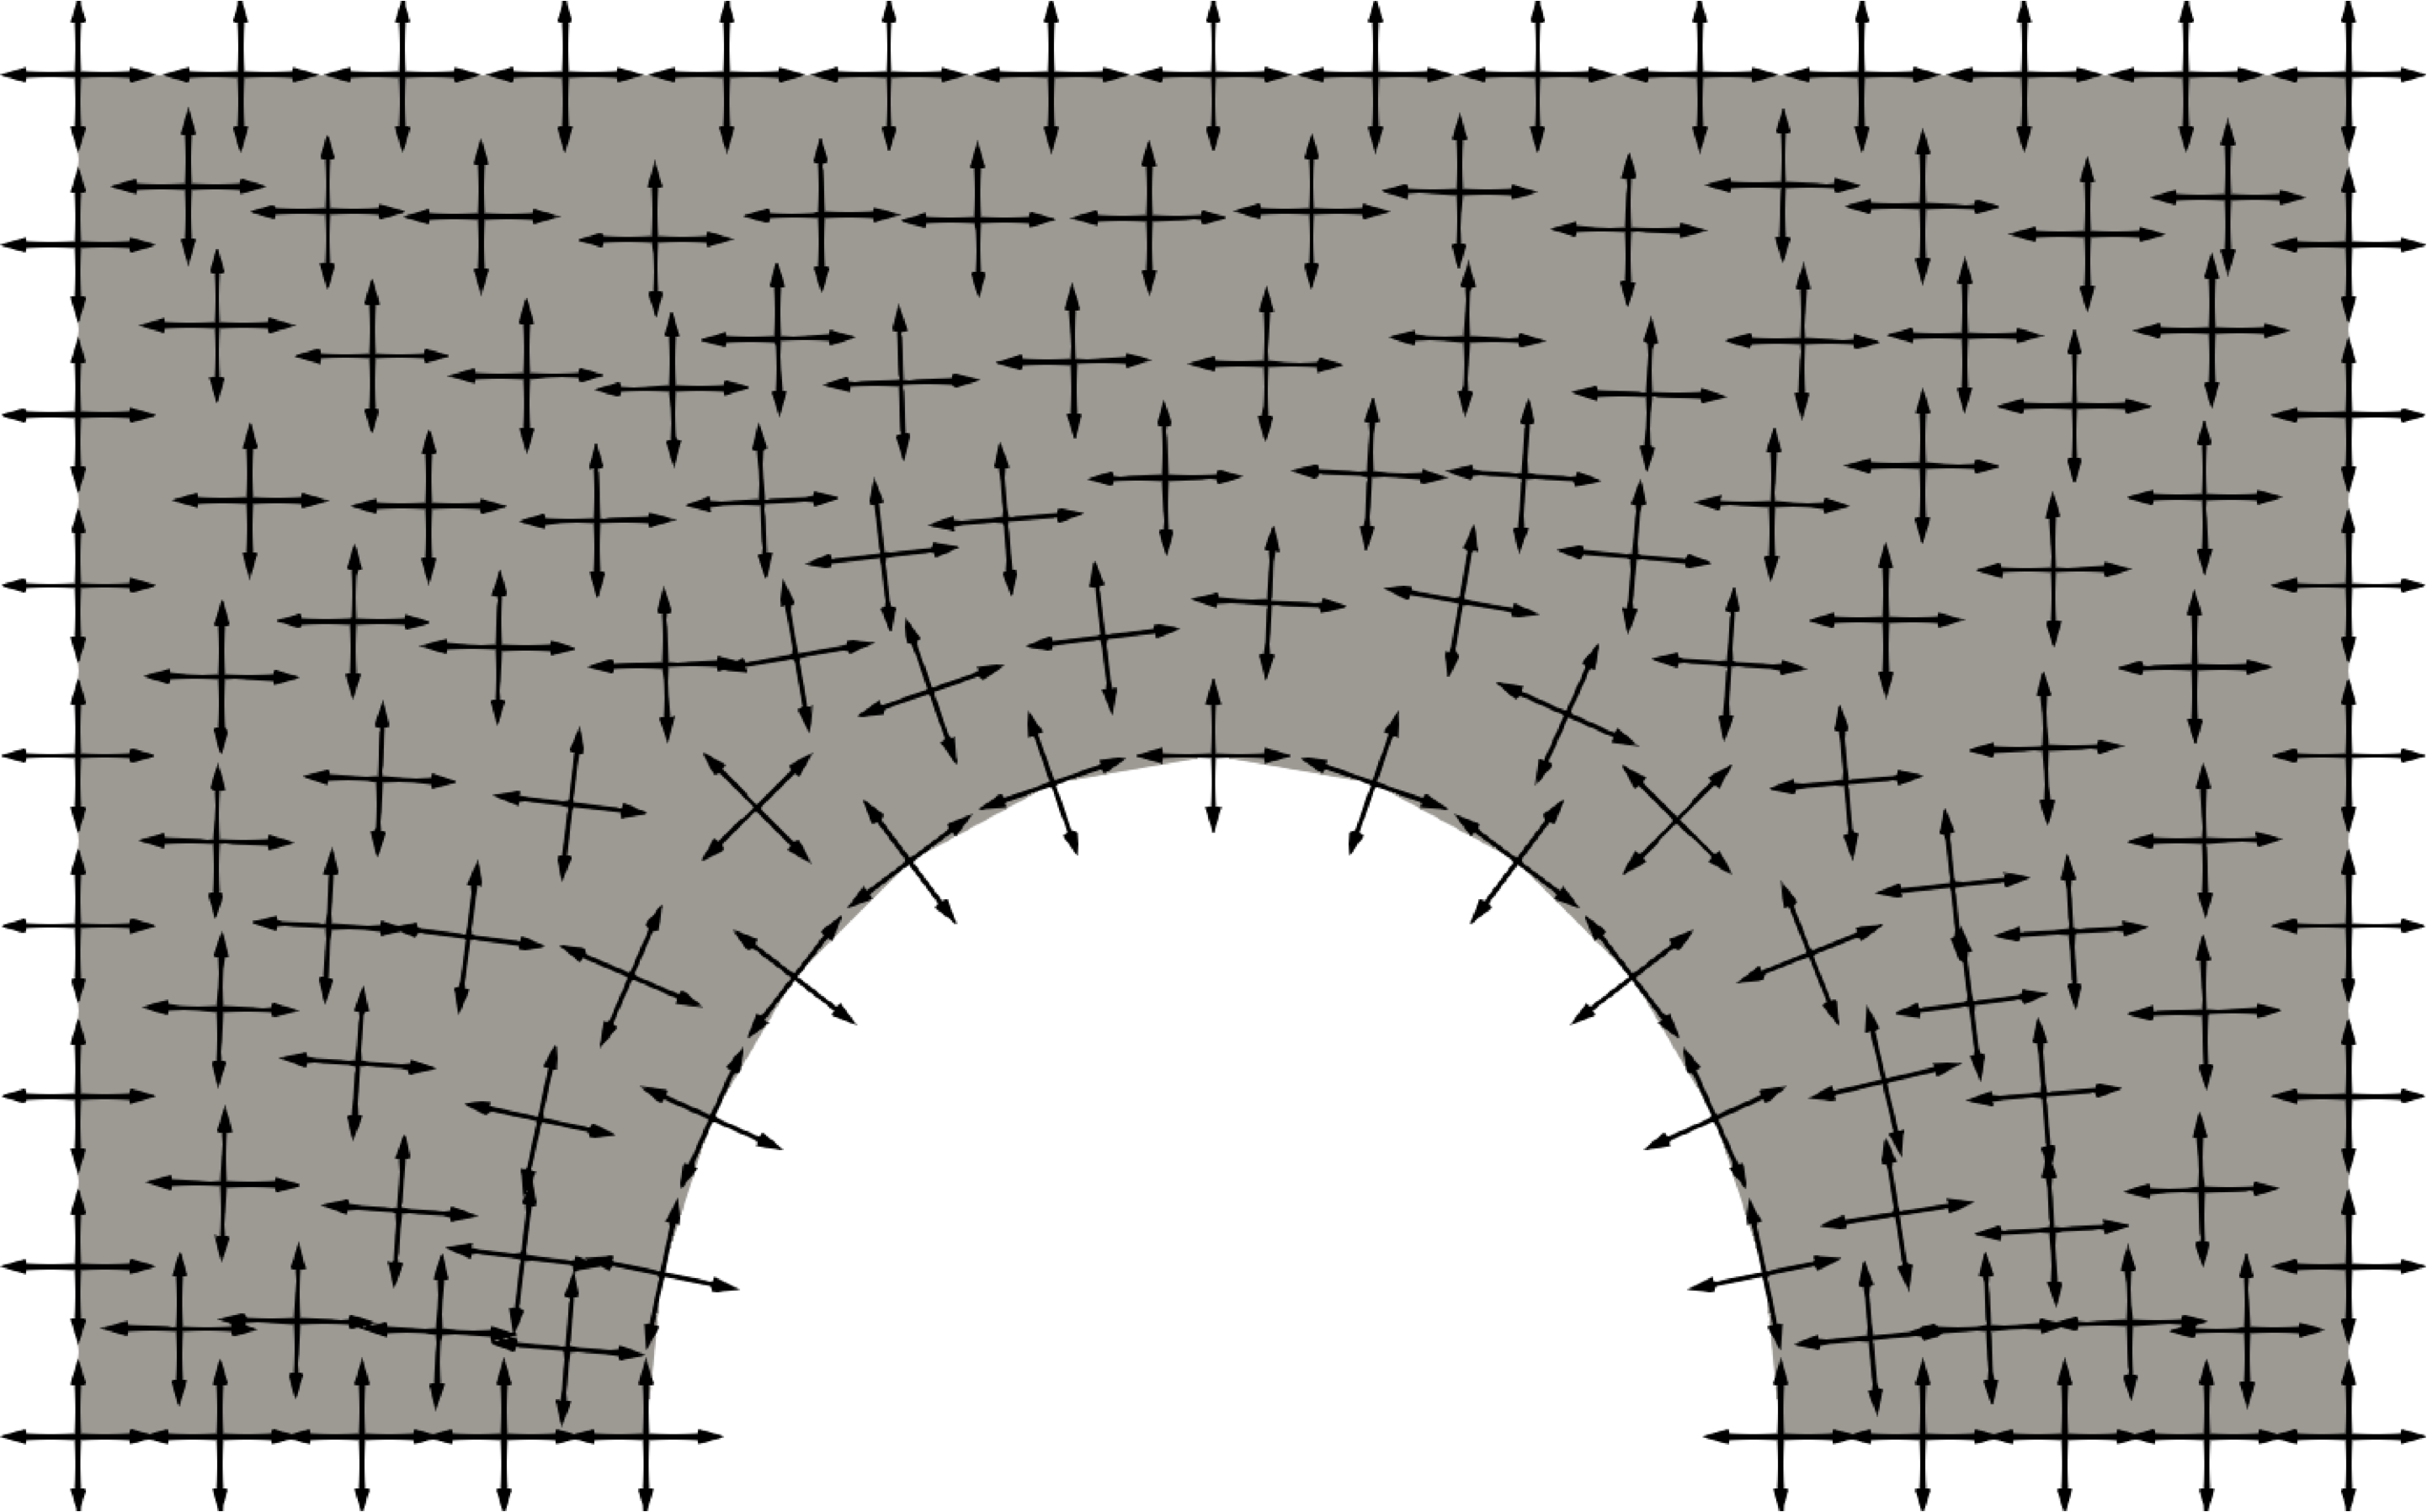
\includegraphics[scale=0.068]{images/frey_4.pdf}\hspace{0.2cm}
\footnotesize Champ de croix
%}
\end{column}

\begin{column}{0.25\textwidth}
\centering
%\onslide<3->{
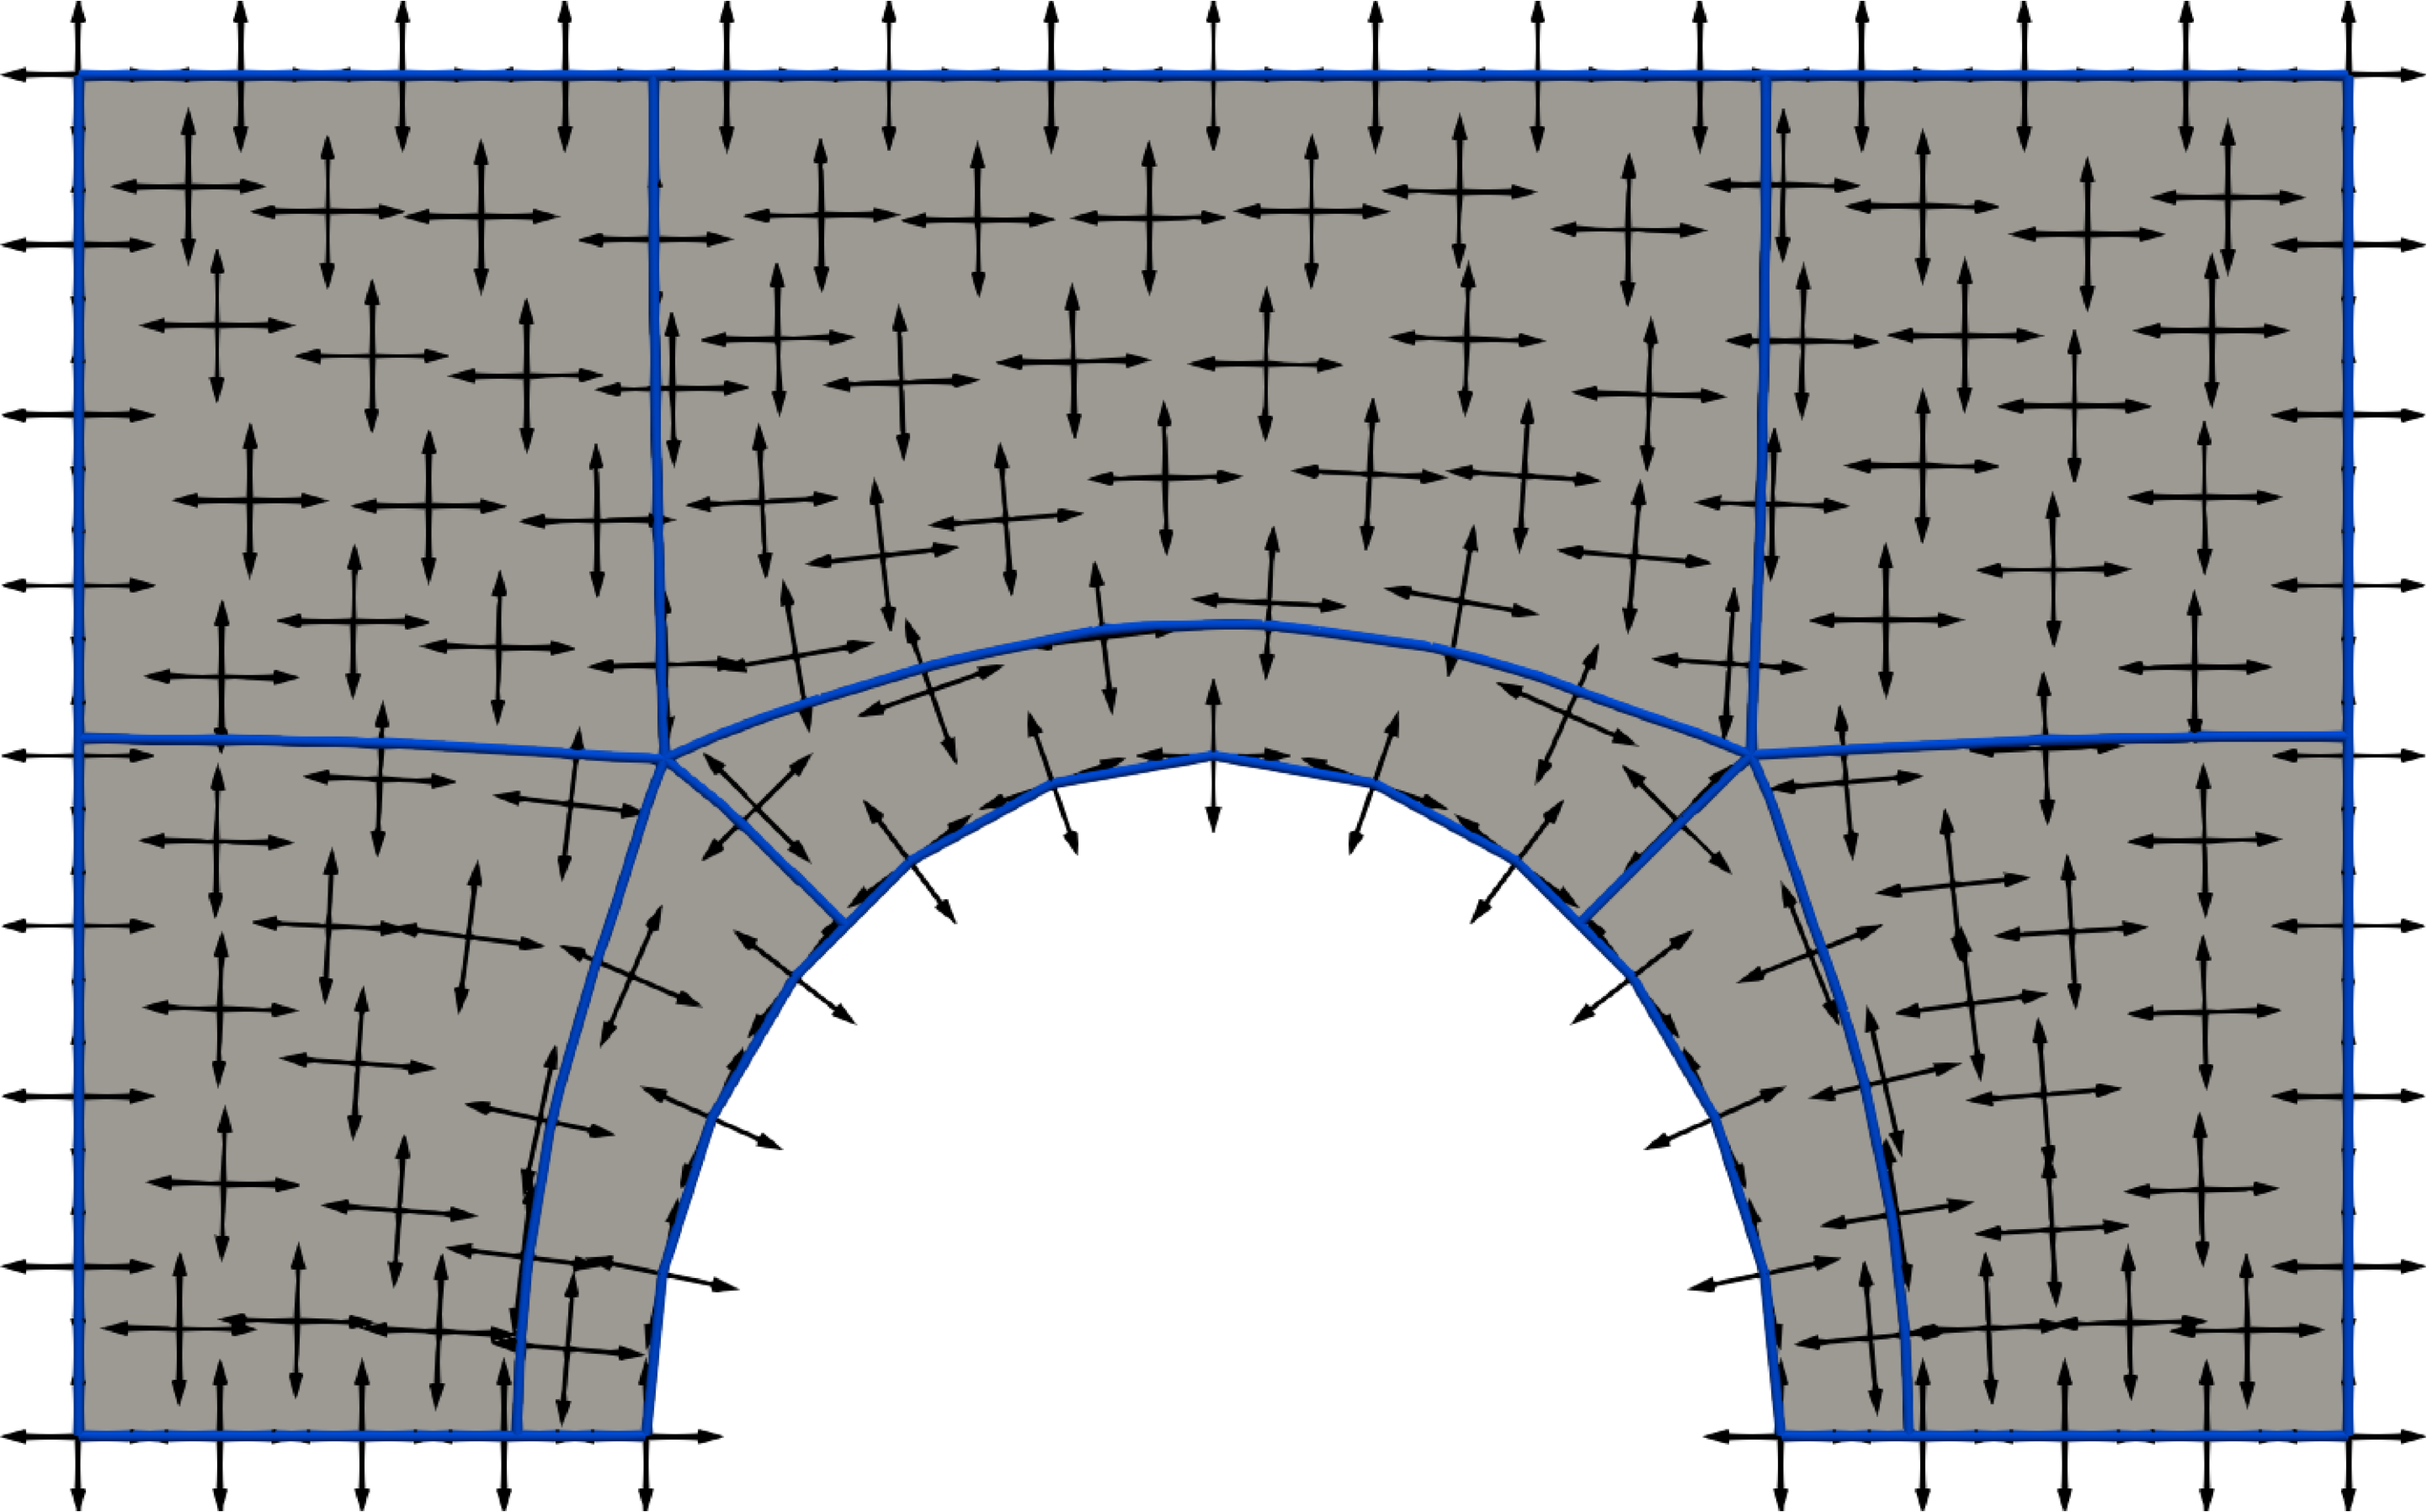
\includegraphics[scale=0.068]{images/frey_5.pdf}\hspace{0.2cm}
\footnotesize Partitionnement
%}
\end{column}

\begin{column}{0.25\textwidth}
\centering
%\onslide<4->{
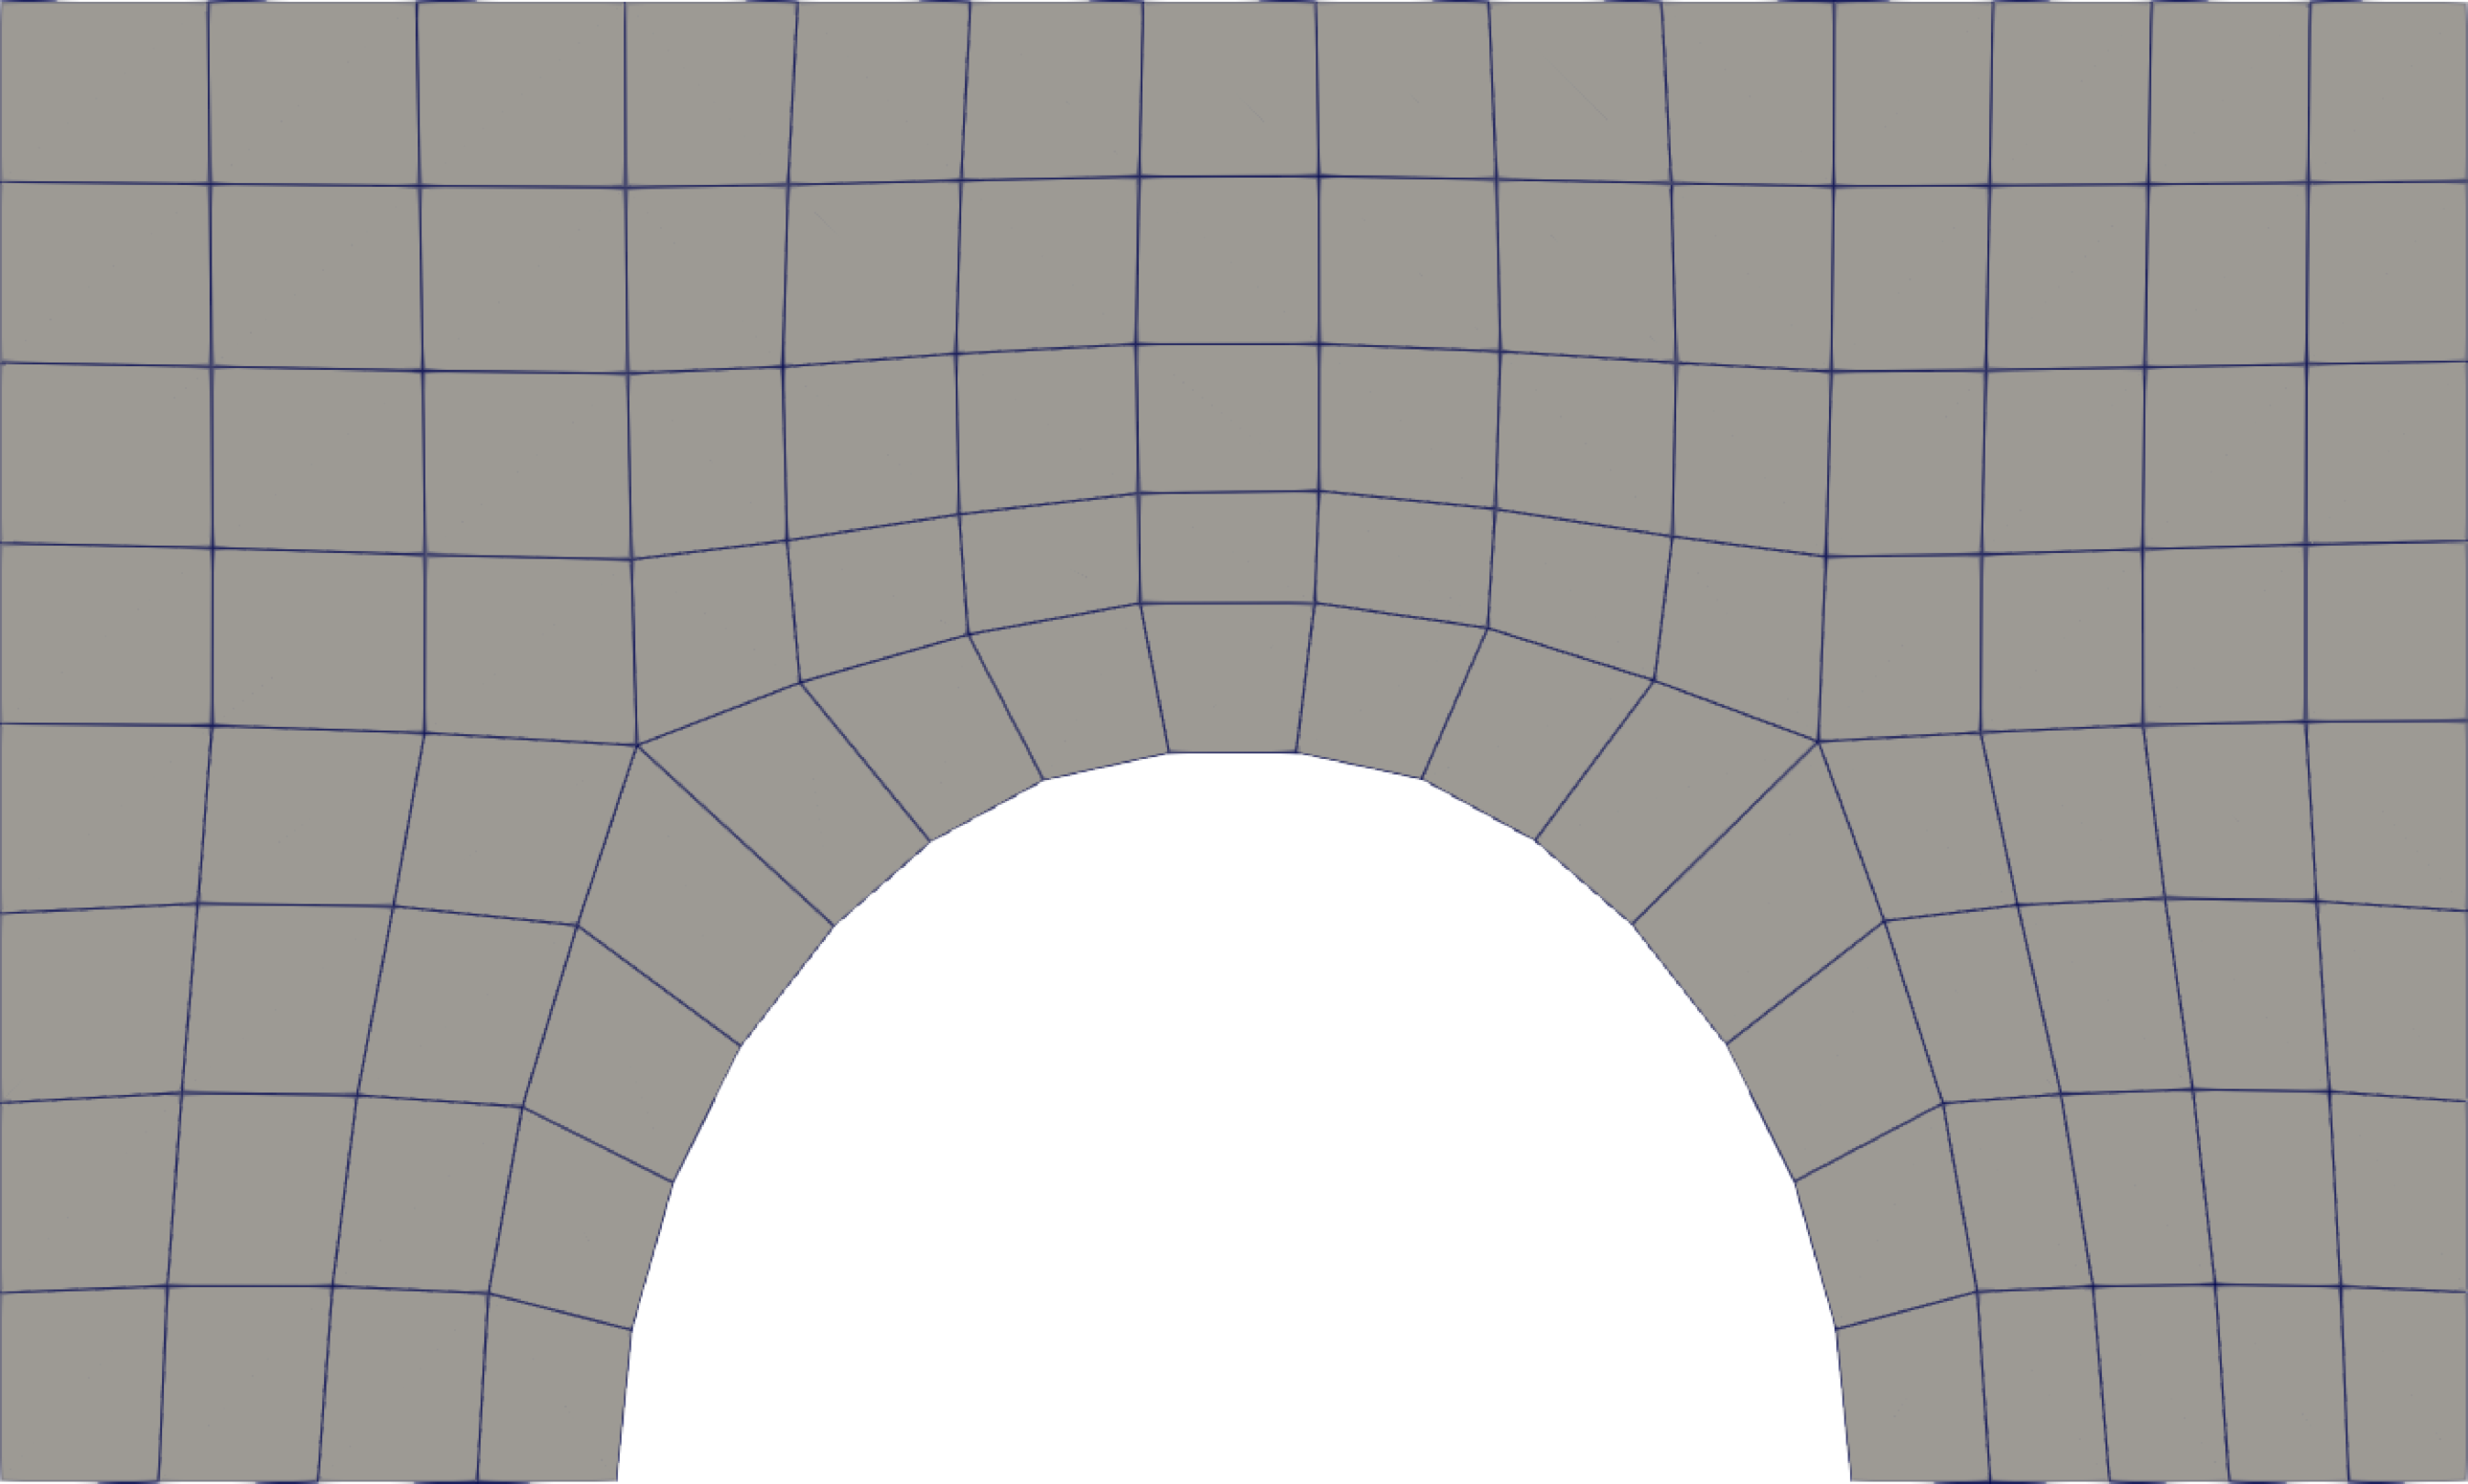
\includegraphics[scale=0.07]{images/frey_6.pdf}\vspace{0.05cm}
\footnotesize Maillage
}
\end{column}

\end{columns}

\vspace{0.4cm}

\begin{columns}
\begin{column}{0.25\textwidth}
\centering
\onslide<2->{
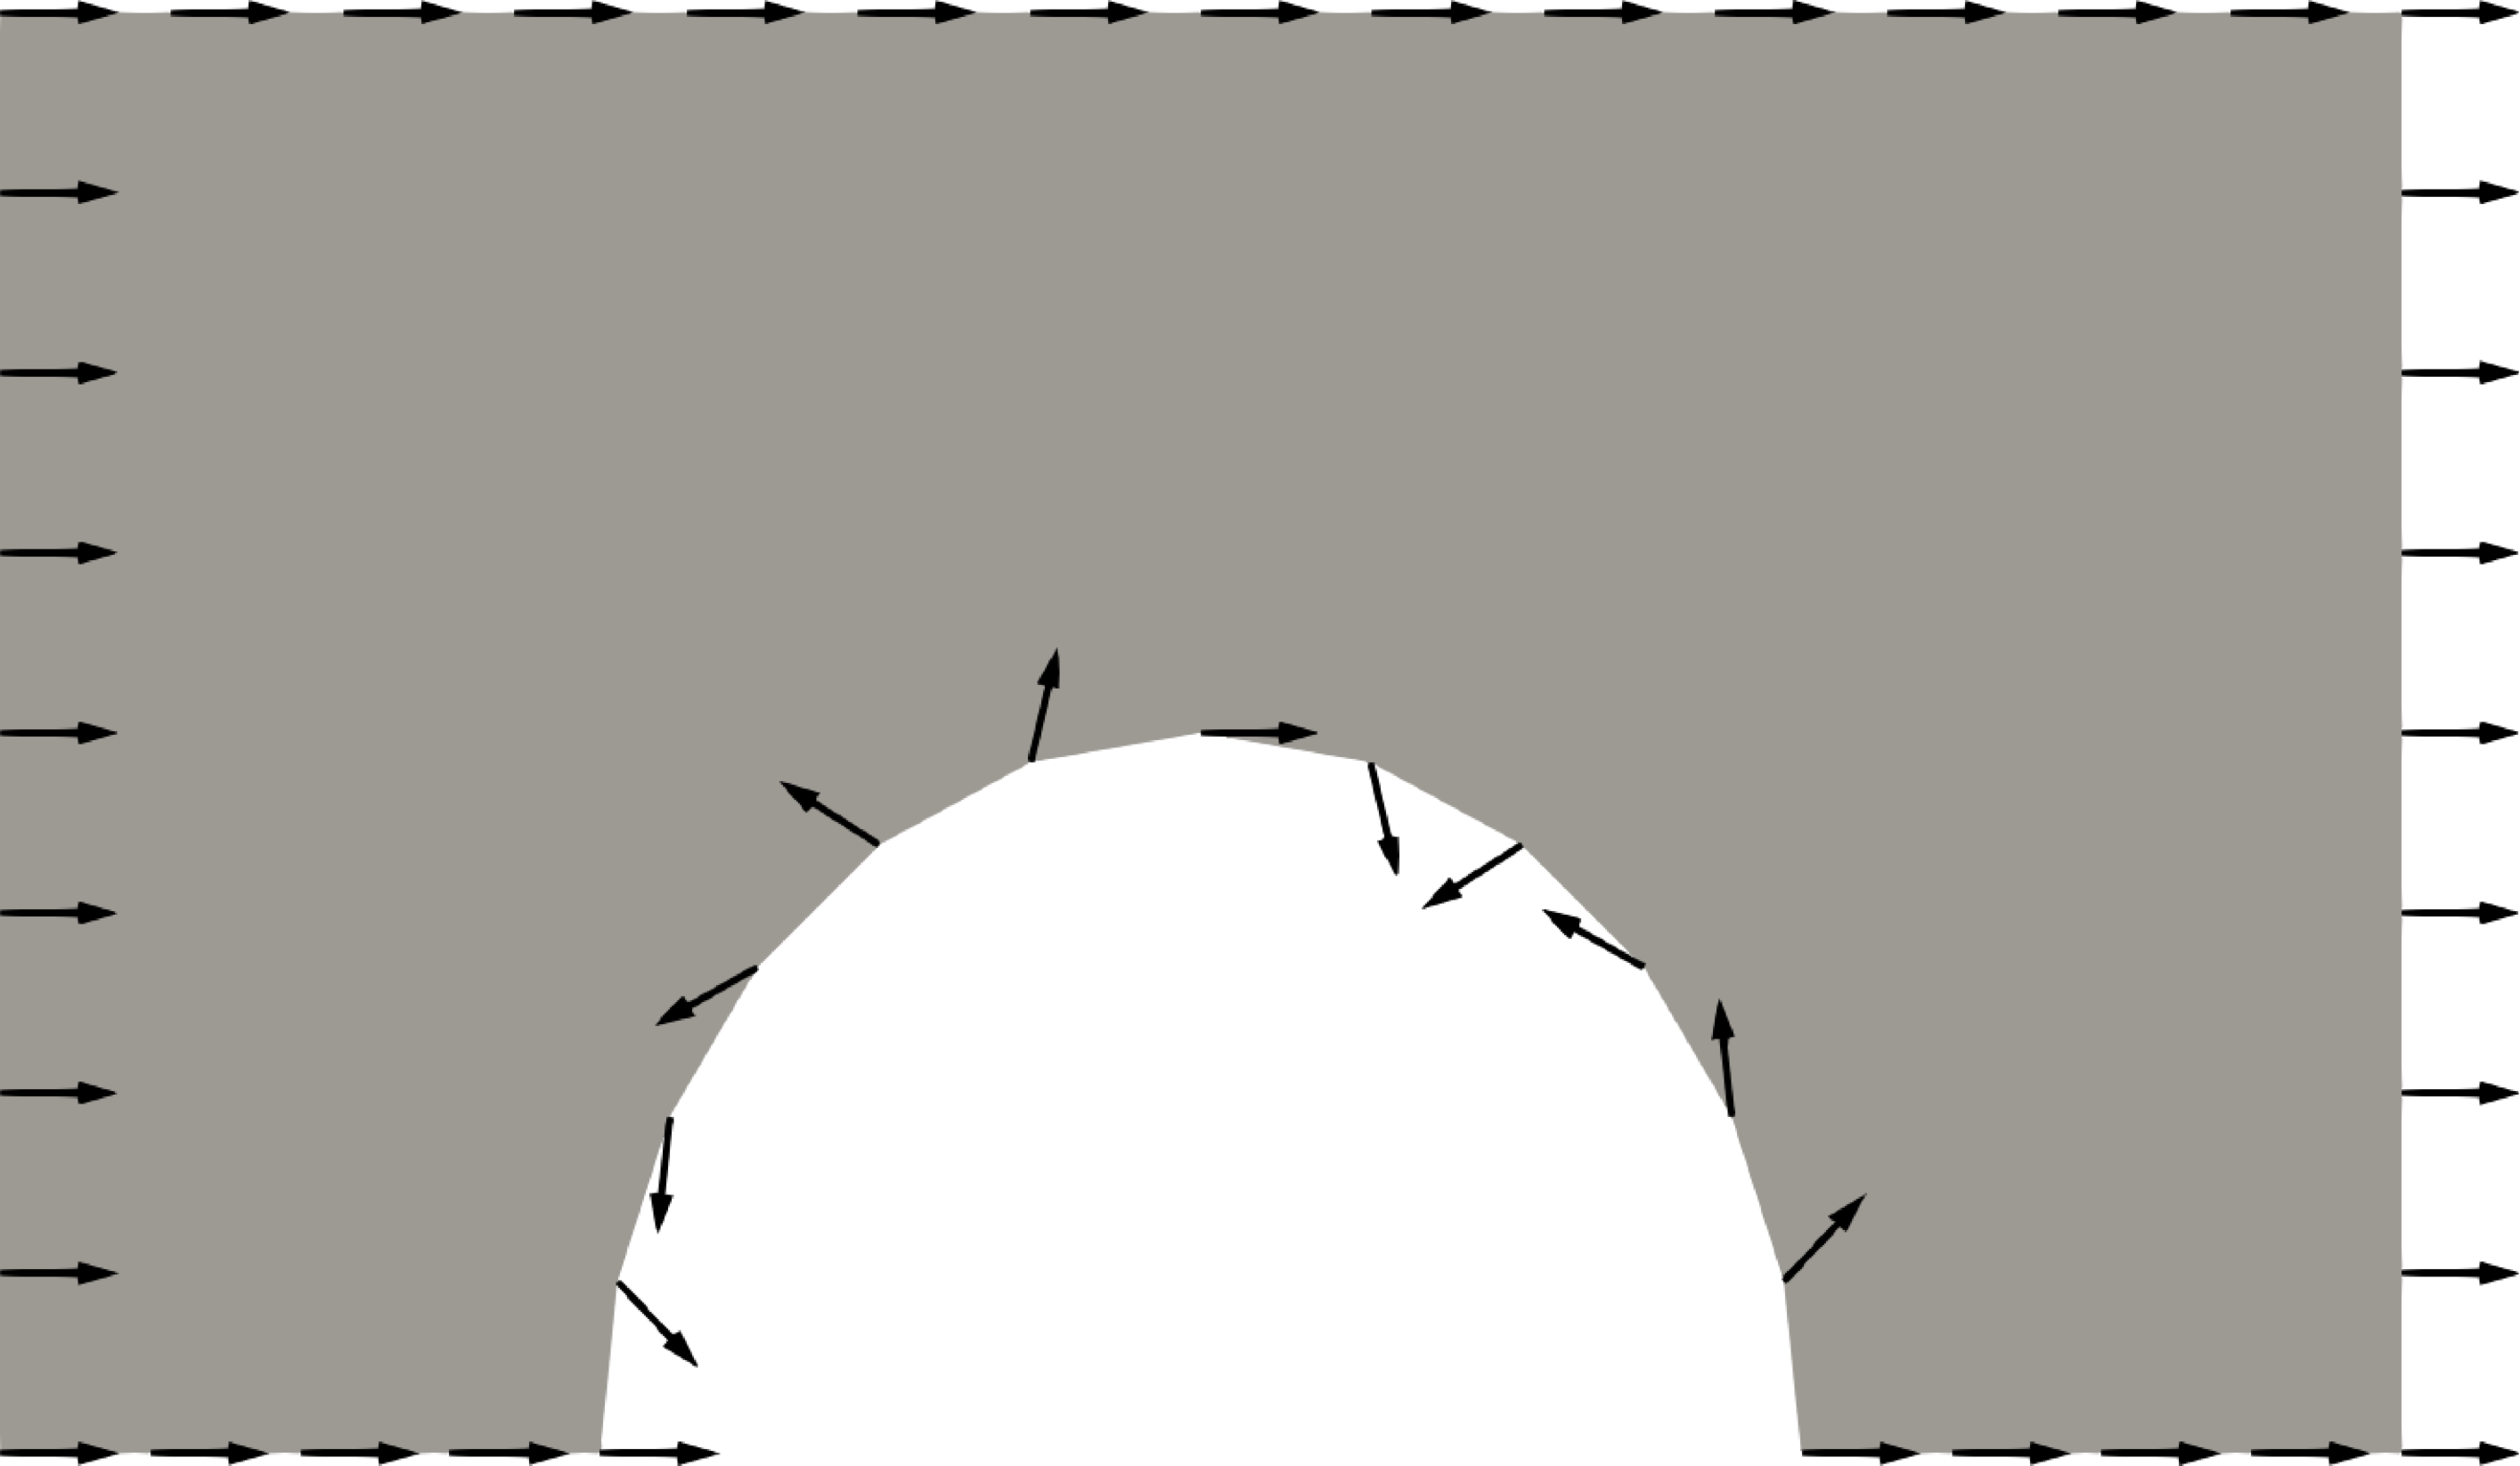
\includegraphics[scale=0.068]{images/frey_2.pdf}\hspace{0.2cm}
%\footnotesize Partitionnement
}
\end{column}
%\pause[2]
\begin{column}{0.25\textwidth}
\centering
\onslide<3->{
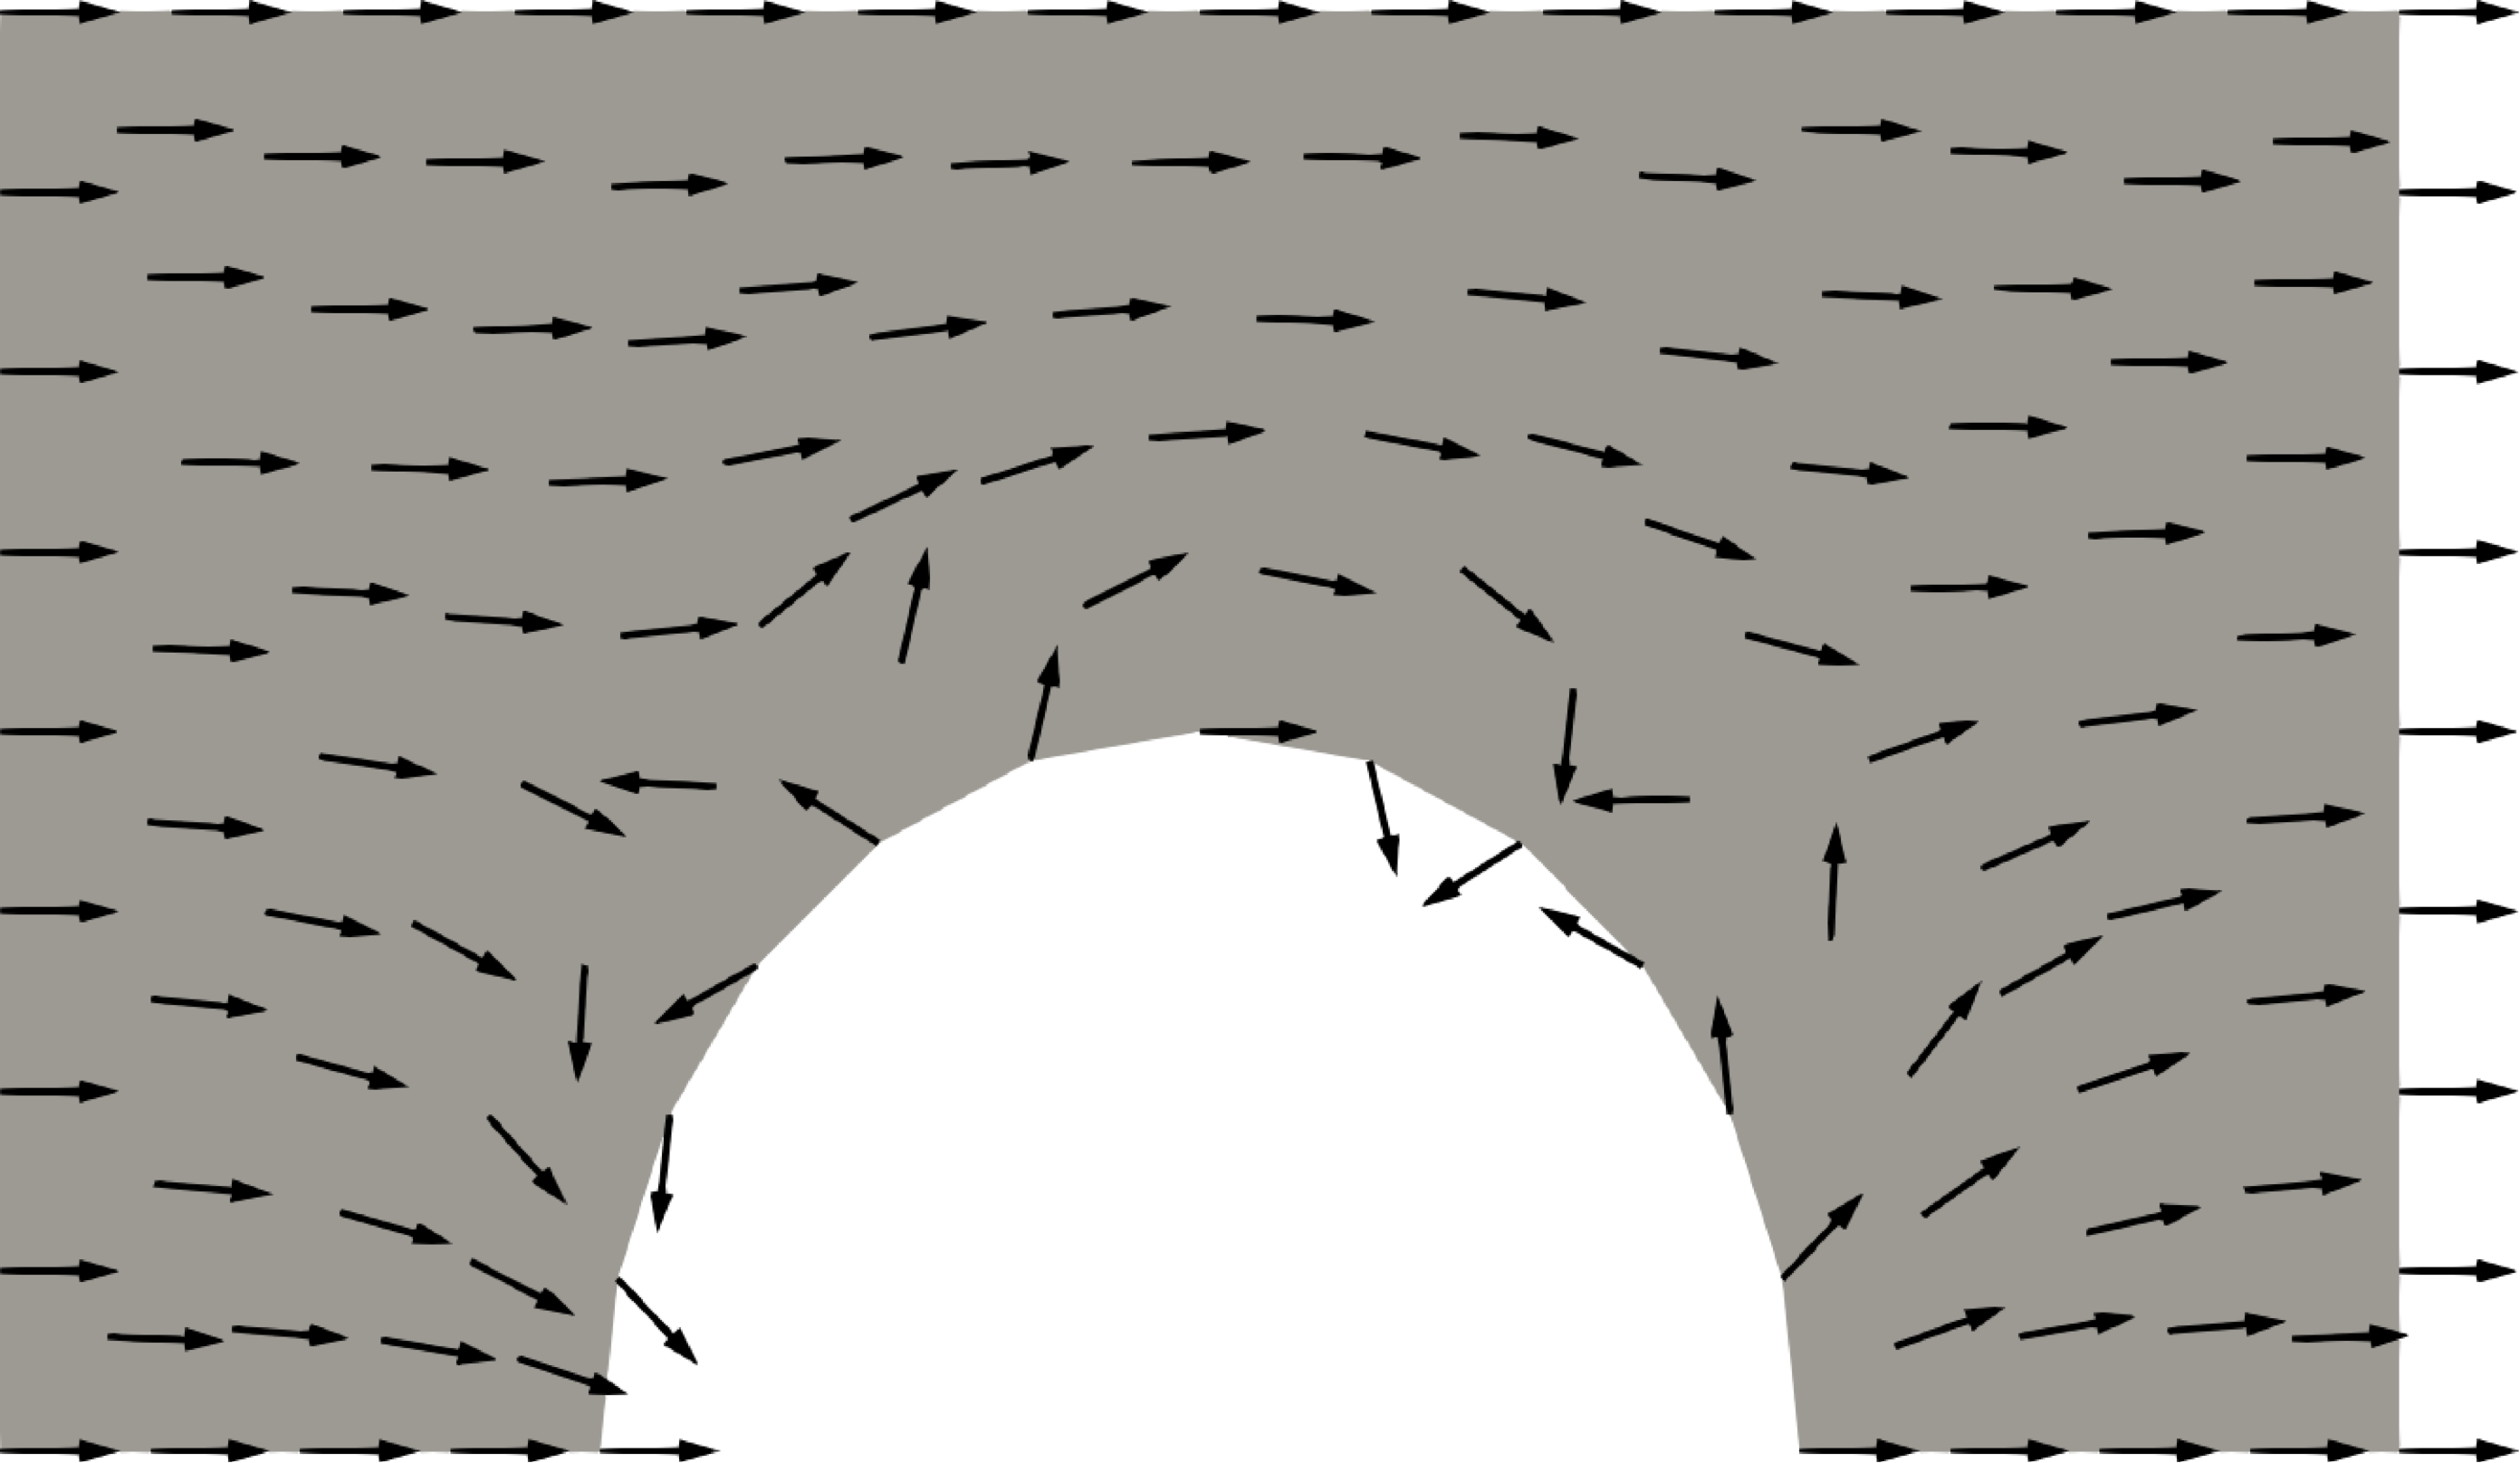
\includegraphics[scale=0.07]{images/frey_3.pdf}%\hspace{0.2cm}
\vspace{0.4cm}
%\footnotesize Maillage
}
\end{column}

%\vspace{0.4cm}

\begin{column}{0.53\textwidth}


\only<2>{
\centering
\begin{itemize}
%\vspace{0.2cm}
\small
\item Une avancée de front à partir de croix {\color{onera_gray} Multivariété des croix, Difficulté d'opérations sur les croix}
%\item $\bar{n}$: champ de croix normal %\\\vspace{0.2cm}
\item $n_r$: champ de représentation normal %\\\vspace{0.2cm}
\item $n_r=(cos(4\theta_{\bar{n}}), sin(4\theta_{\bar{n}}))$
\end{itemize}
}


\only<3>{
\small
{\color{onera} Diffusion du champ de représentation:} {\color{onera_gray} Equation de Laplace [Kowalski et al. (2013)], Minimisation de l'énergie de Ginzburg-Landau [Viertel et al. (2018)]}%\vspace{0.2cm}
\begin{equation*}
    \left\{
    \begin{array}{lcll}
    \triangle u_r&=&0&\mbox{ dans }\Omega,\\\\
    u_r&=&n_r&\mbox{ sur }\partial\Omega.
    \end{array}
    \right.
\end{equation*}
}

\only<4>{
\small
{\bf Avantages:}
\begin{itemize}
\item blocs structurés: {\color{onera_gray}faible stockage, connectivité efficace.}%, calcul parallèle.}
\item qualités des éléments: {\color{onera_gray} topologiquement proche de carré, de rectangle, convexe.}
\item suivi de la frontière: {\color{onera_gray} fidèle à la CAO.}%, récupération automatique de la frontière.}
\item faible nombre de sommets irréguliers
\vspace{0.4cm}
\end{itemize}
}
\end{column}
\end{columns}

%\pause
%\begin{columns}
%\begin{column}{0.45\textwidth}
%\pause[1]
%{\color{onera} Génération du champ de croix:} {\color{onera_gray} Minimisation de l'énergie de Ginzburg-Landau [Viertel et al. (2018)]}\vspace{0.2cm}
%$$
%\displaystyle\inf_{u} E(u)=\displaystyle\frac{1}{2}\int_\Omega|\nabla u|^2dA+\frac{1}{4\epsilon^2}\int_\Omega(|u|^2-1)dA.
%$$
%\end{column}

%\end{columns}
\end{frame}


\begin{frame}
\frametitle{Une approche basée sur les champs de croix}
\small
\begin{columns}
    \begin{column}{0.55\textwidth}
    \only<1>{
    {\bf Les limites de cette approche:}\vspace{0.2cm}
        \begin{itemize}
            \item {\color{onera} Génération du champ de croix:} non-contrôle de la position des points singuliers, abscence de notion de point singulier de bord, non-homogénéité\vspace{0.2cm}
            \item {\color{onera} Domaine très étiré:} tend à produire des champs de croix contenant des points singuliers non isolés\vspace{0.2cm}
            \item {\color{onera} Analyse de la méthode:} approche Ginzburg-Landau, analyse complexe, {\color{onera_gray}[Viertel et al (2020)]}  \vspace{0.2cm}
            \item {\color{onera} Variété surfacique sans bords}
        \end{itemize}
    }

        \only<2>{
    {\bf Idée:} Mettre en place un processus permettant d'aboutir à des mesh quad à partir de champs de croix arbitraires\vspace{0.3cm}
        \begin{itemize}
            \item Choisir un champ de croix ayant des caractéristiques plus convenable \vspace{0.3cm}
            \item Analyse théorique de la méthode pour comprendre la formation des partitions à 4 côtés.
        \end{itemize}
    }

    \end{column}
    \begin{column}{0.45\textwidth}
        \centering
        \vspace{-0.15cm}
        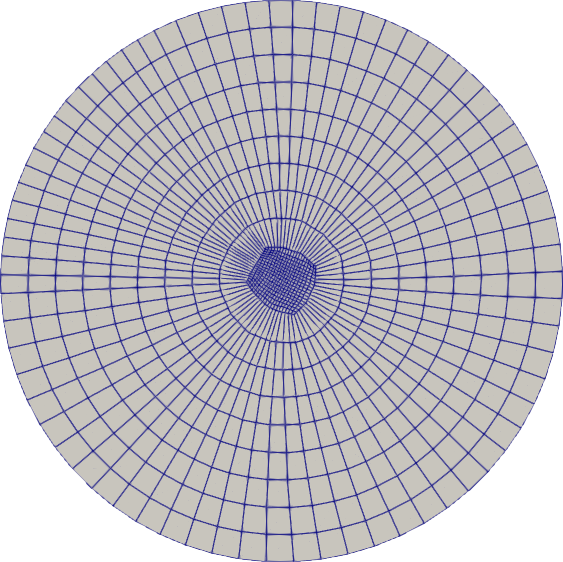
\includegraphics[scale=0.12]{images/new_cercle.png}
        \hspace{0.6cm}
        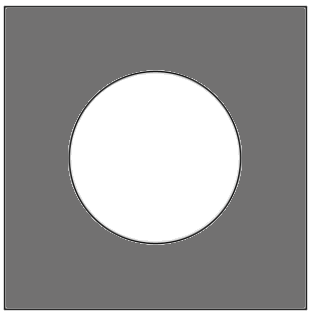
\includegraphics[scale=0.28]{images/carreTrou.png}
        \\\vspace{0.2cm}
        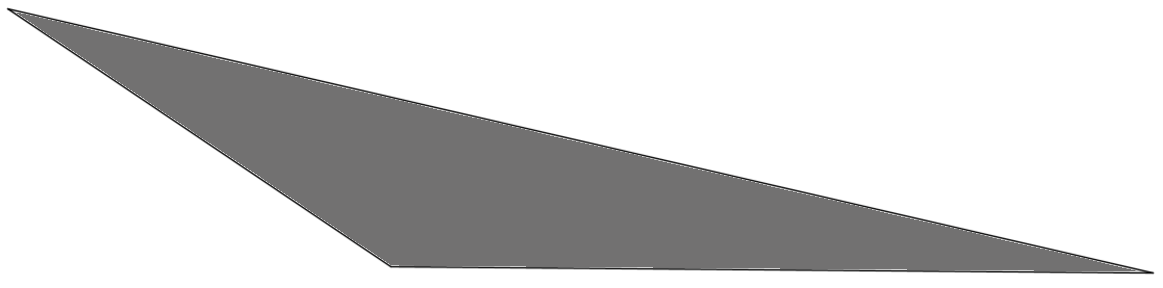
\includegraphics[scale=0.18]{images/triangle_etire.png}
        \hspace{0.2cm}
        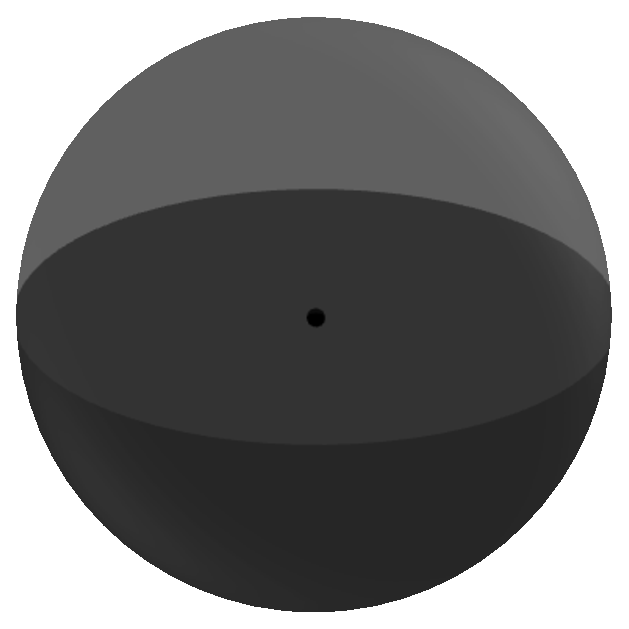
\includegraphics[scale=0.23]{images/sphere.eps}
        \vspace{0.3cm}
    \end{column}
\end{columns}
\end{frame}


\begin{frame}{Plan}
    %\tableofcontents
    \vspace{-0.4cm}
    \begin{enumerate}
        \item \color{onera} Contexte et objectifs \\\vspace{0.26cm}
        \item Formalisation du processus de partitionnement %{\color{onera_gray}(nouveau point de vue, redressement du champ sur le bord, ...)}
        \vspace{0.26cm}
        \begin{itemize}
            \item Prise en compte de champs de croix arbitraires\\\vspace{0.18cm}
            \item Processus d'alignement\\\vspace{0.18cm}
            \item Domaines non-simplement connexes\\\vspace{0.18cm}
            \item Discussions (quelques résultats théoriques)\\\vspace{0.18cm}
            %\item Exemples%\\\vspace{0.2cm}
        \end{itemize}
        %\item Traitement des singularités de bord {\color{onera_gray}(prise en compte de conditions de bord, ...)}\\\vspace{0.5cm}
        %\item Prise en compte de champs de croix arbitraires {\color{onera_gray}(domaine à trous, multimatériau, ...)}\\\vspace{0.34cm}
        \item Discrétisation et extension aux variétés surfaciques non-planaire %{\color{onera_gray}(prise en compte de la courbure, généralisation, ...)}\\
        \vspace{0.26cm}
        \begin{itemize}
            \item Processus de partitionnement\\\vspace{0.18cm}
            \item Analyse de convergence\\\vspace{0.18cm}
            %\item Exemples%\\\vspace{0.2cm}
        \end{itemize}
        \item Conclusion et perspectives
    \end{enumerate}
\end{frame}


\begin{frame}{Prise en compte de champs de croix arbitraires}
\small
Une {\color{onera}croix} est un élément de l'ensemble quotient $\mathbb{S}^1/\mathcal{Q}\cup\{0\}$ {\color{onera_gray}(cercle unité, ensemble de 4 vecteurs)}.\\\vspace{0.2cm}
Un {\color{onera}champ de croix} est une application $\bar{u}:p\in\Omega\rightarrow \bar{u}(p)\in S^1/\mathcal{Q}\cup\{0\}$.\\\vspace{0.2cm}

\begin{onerablock}[drop fuzzy shadow]{\small Définition}
\small
$\bar{u}$ est un champ de croix \emph{presque-$\mathcal{C}^1$} si $\bar{u}$ est de classe $\mathcal{C}^1$ en tout point sauf en un nombre fini de point {\color{onera_gray}(les points singuliers)}.
\end{onerablock}

{\bf\underline{Exemple:}} {\color{onera_gray} champ de croix à partir d'un mode propre du laplacien sur le demi-disque. Tangente et gradient des isolines. Pts. sing. et extrémas. Quart de l'angle des croix. Partitionnement. Outil.}



    \begin{columns}
        \begin{column}{0.33\textwidth}
        \centering
\onslide<2->{
        %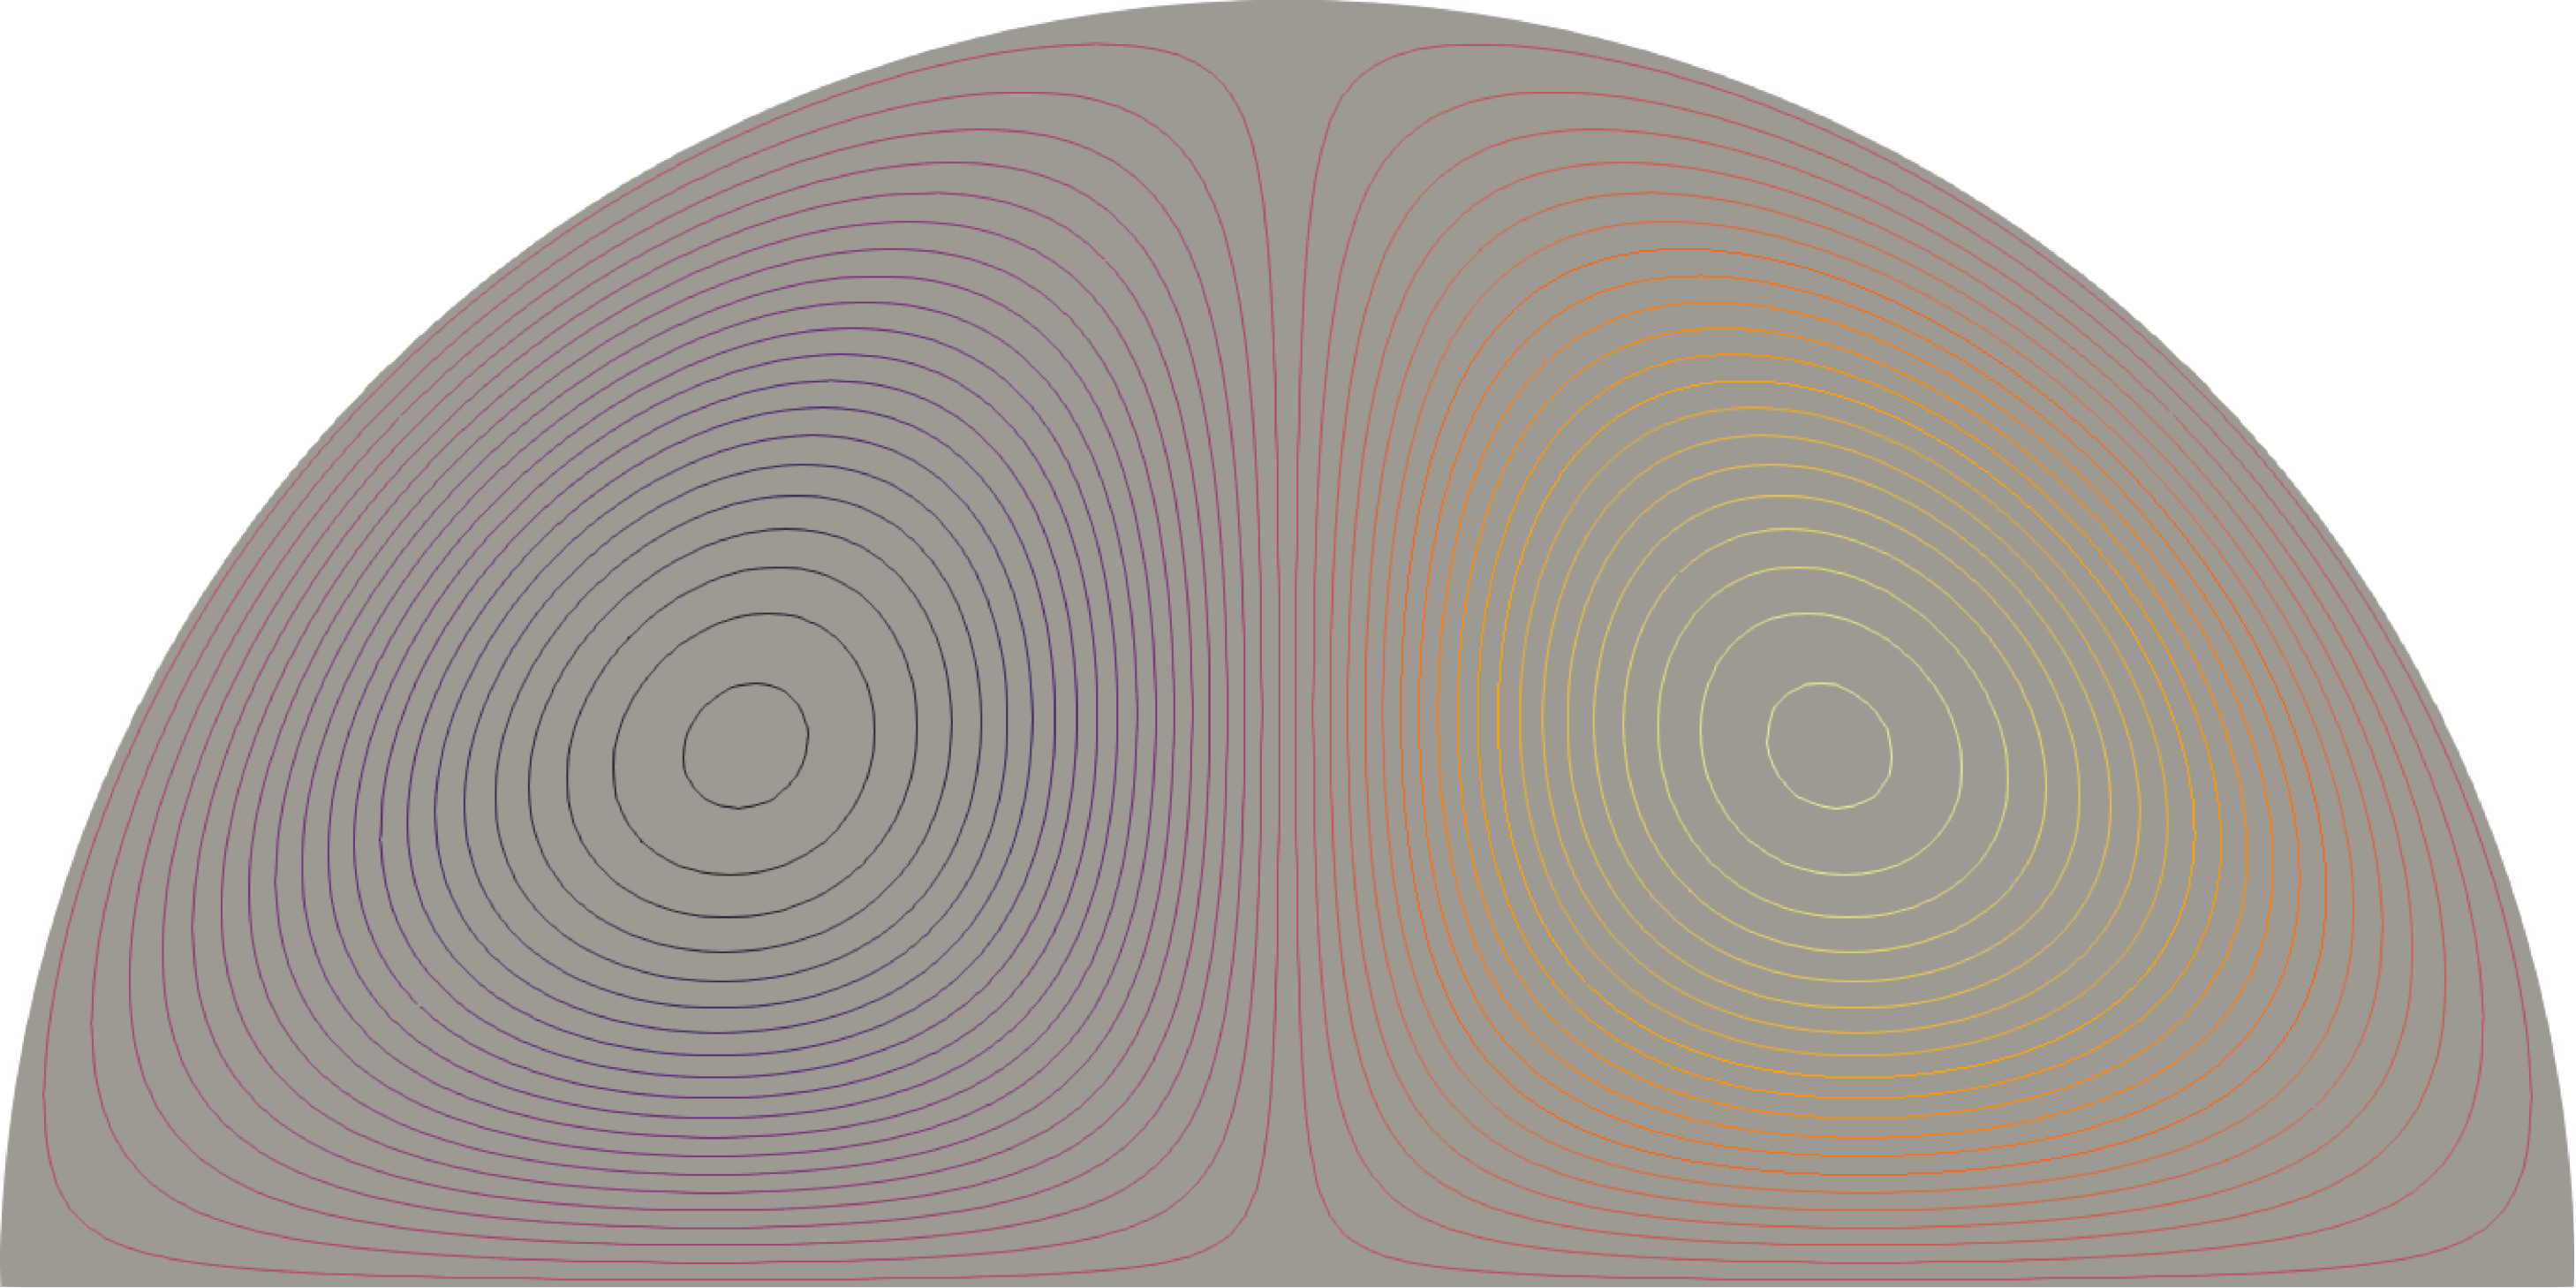
\includegraphics[scale=0.091]{images/mode_prop.pdf}
        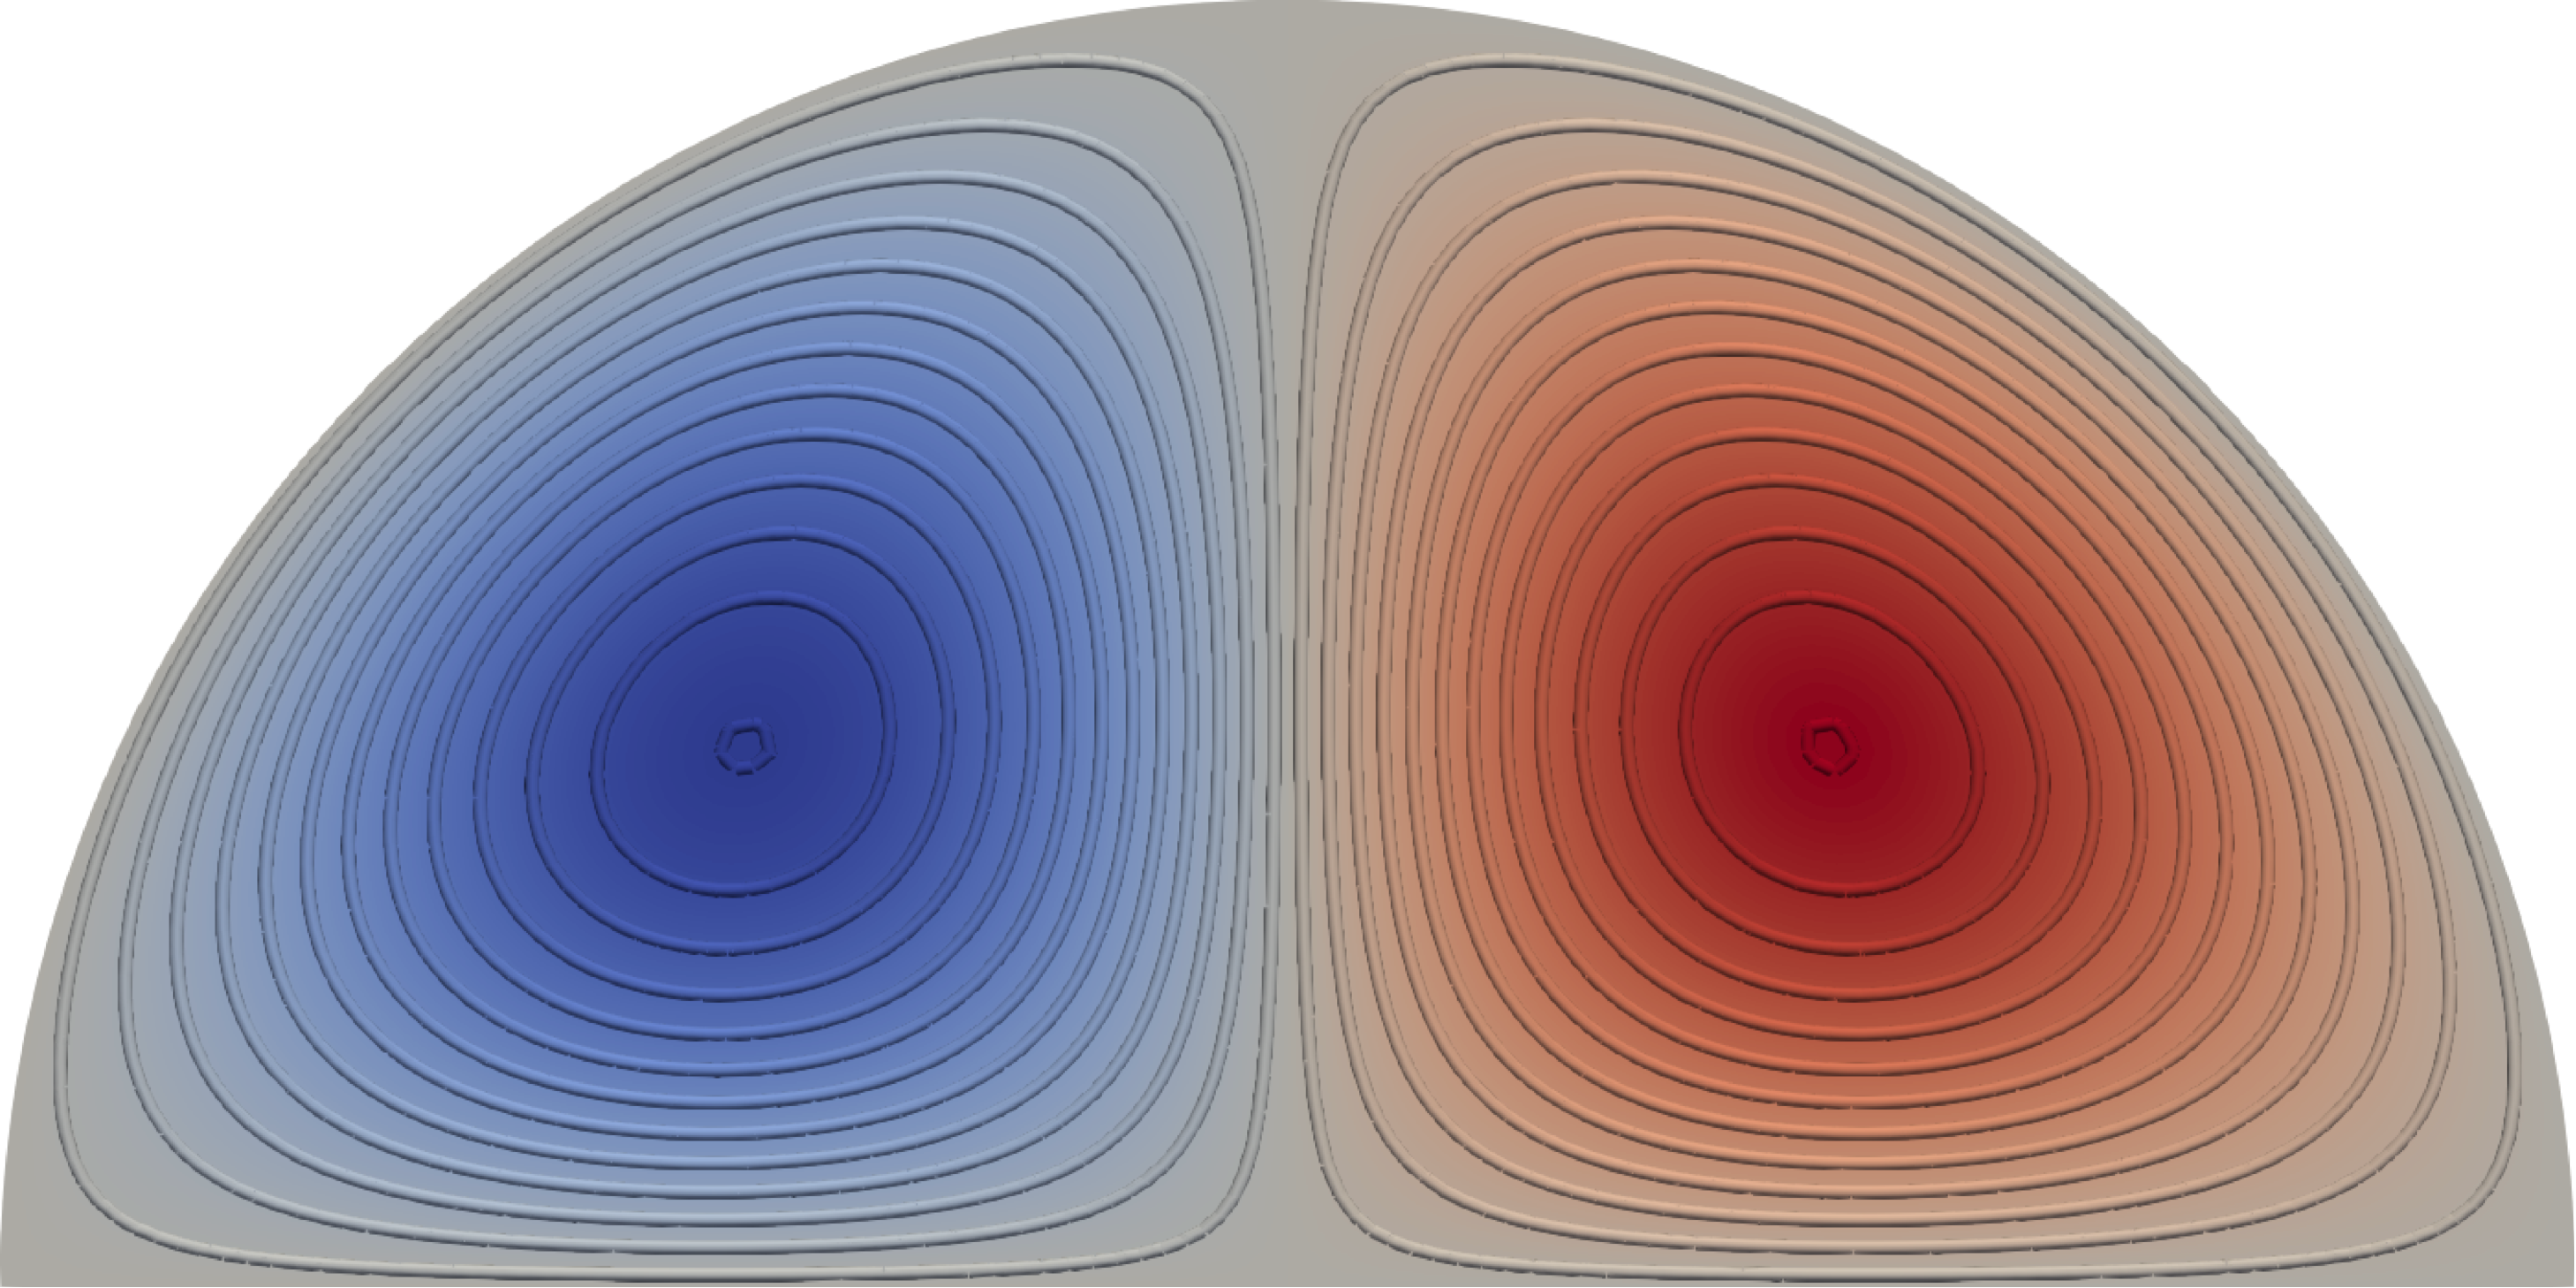
\includegraphics[scale=0.092]{images/mode_prop_new.pdf} \hspace{0.2cm}
        %\footnotesize Mode propre du laplacien sur le demi-disque
%        }
        \end{column}
        \begin{column}{0.33\textwidth}
        \centering
%\onslide<2->{
        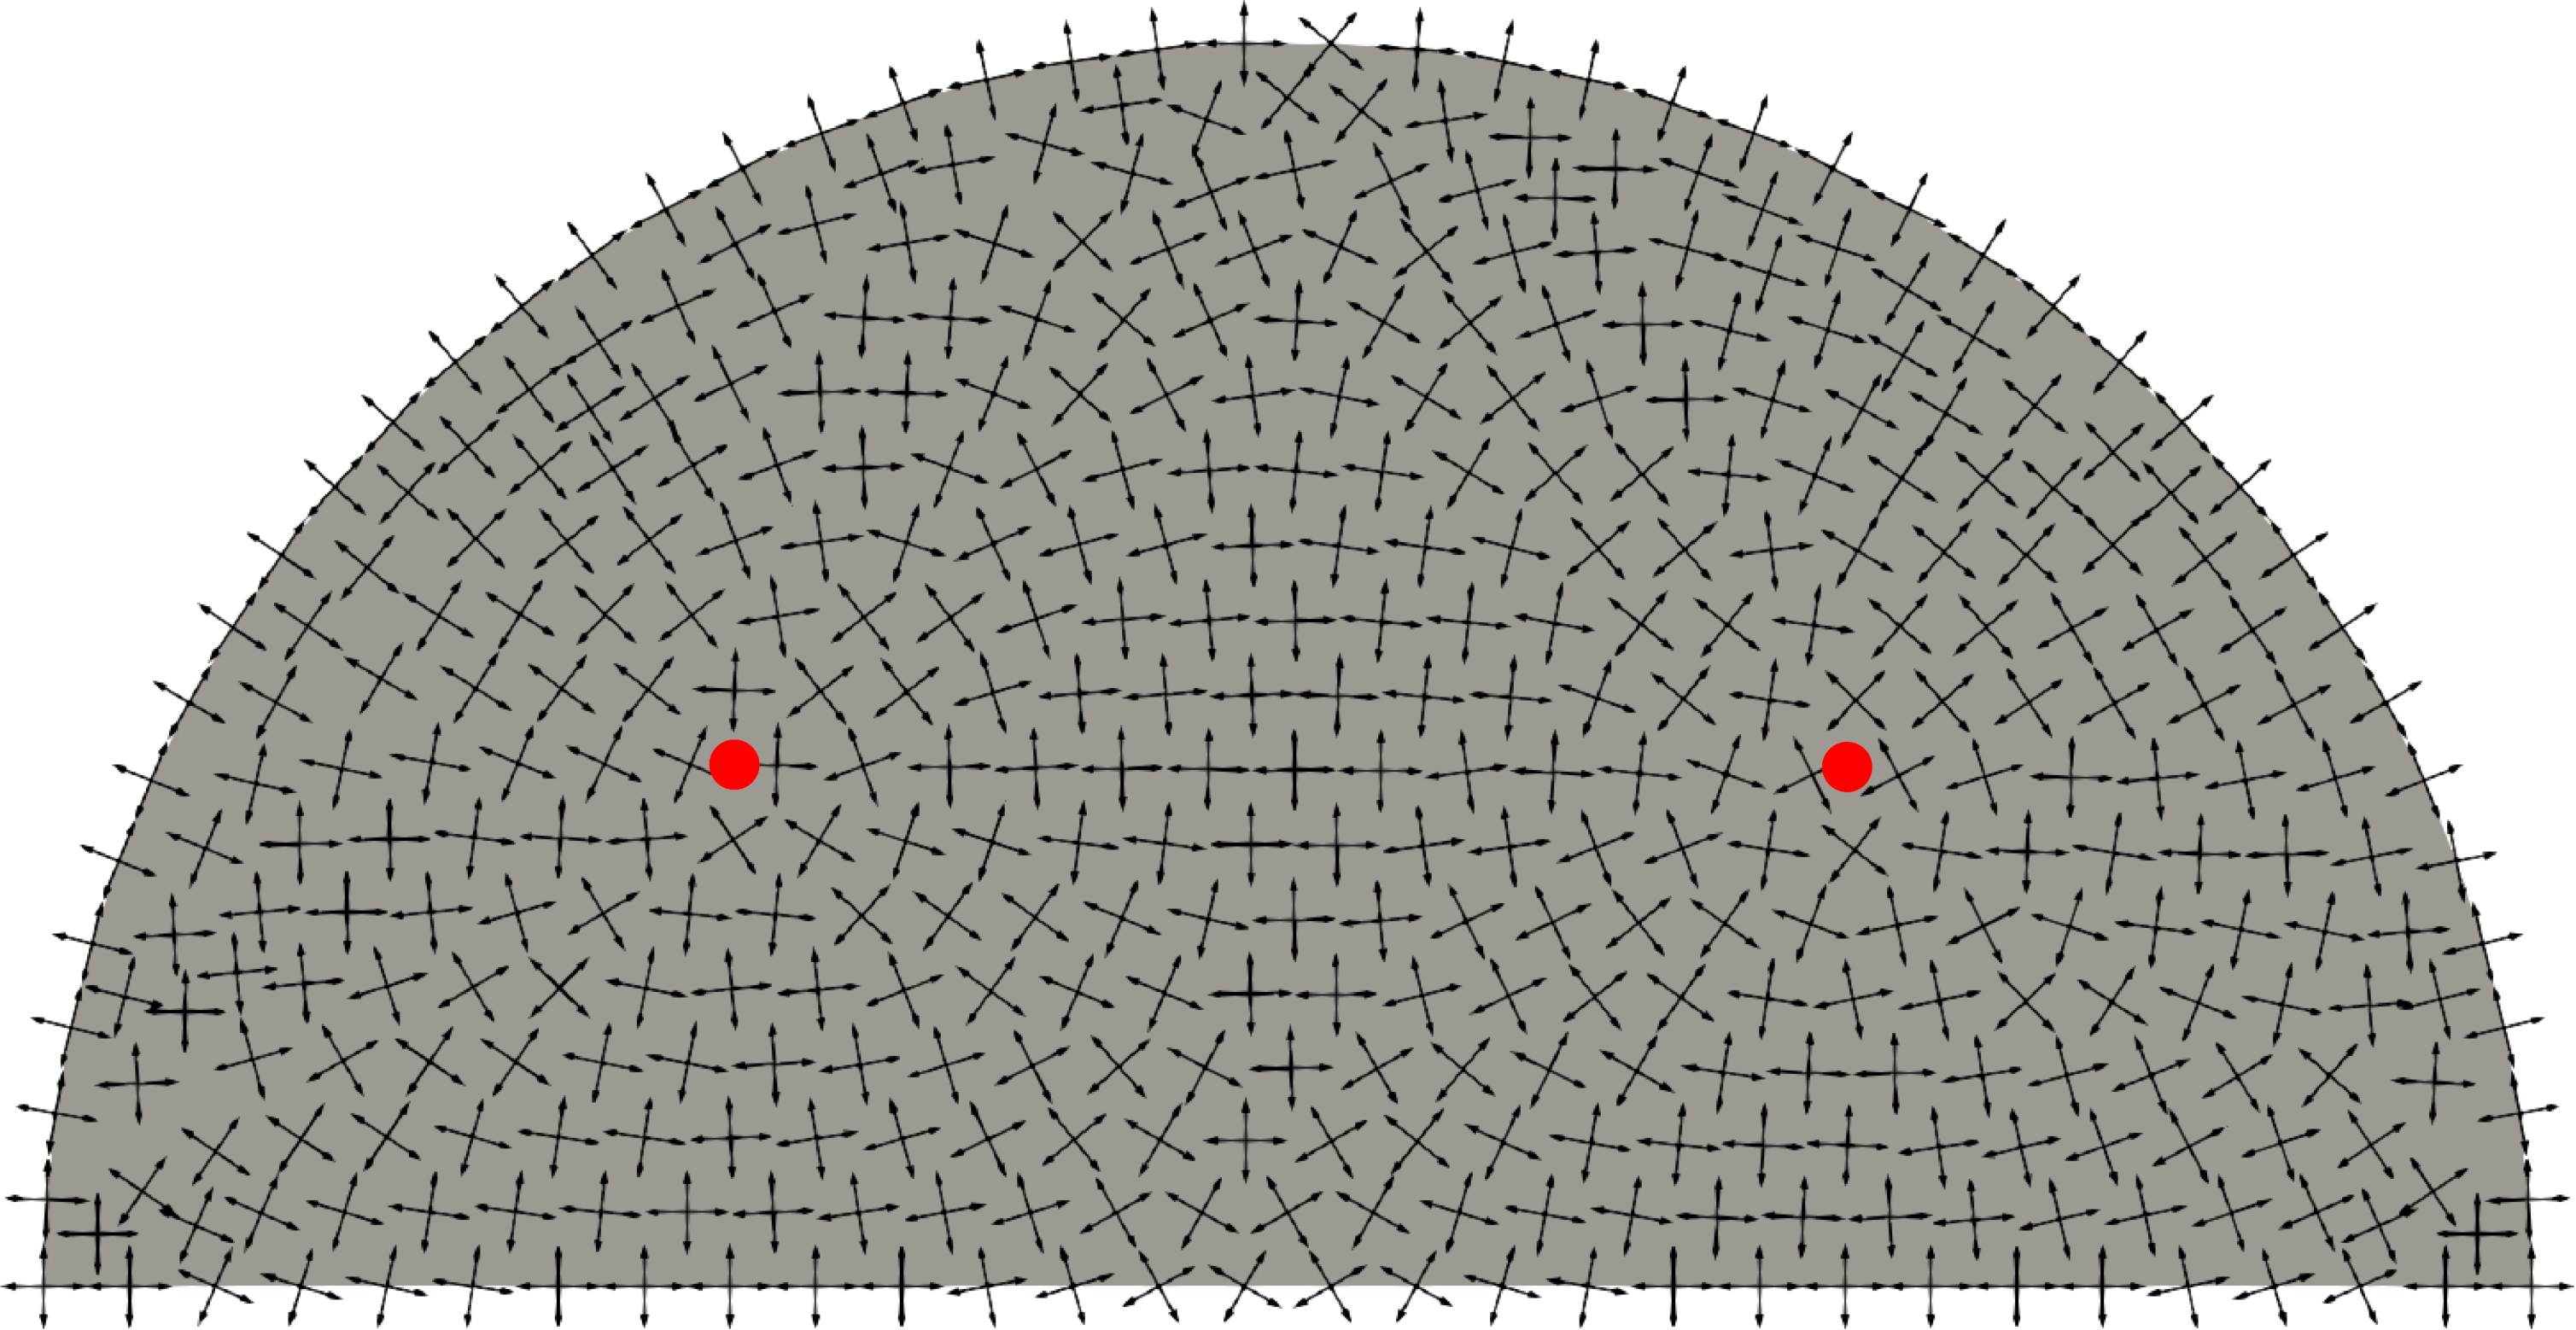
\includegraphics[scale=0.092]{images/tang_grad.pdf} \hspace{0.2cm}
        %\footnotesize Tangentes aux lignes de niveaux
        }
        \end{column}
        \begin{column}{0.33\textwidth}
        \centering
\only<3>{
        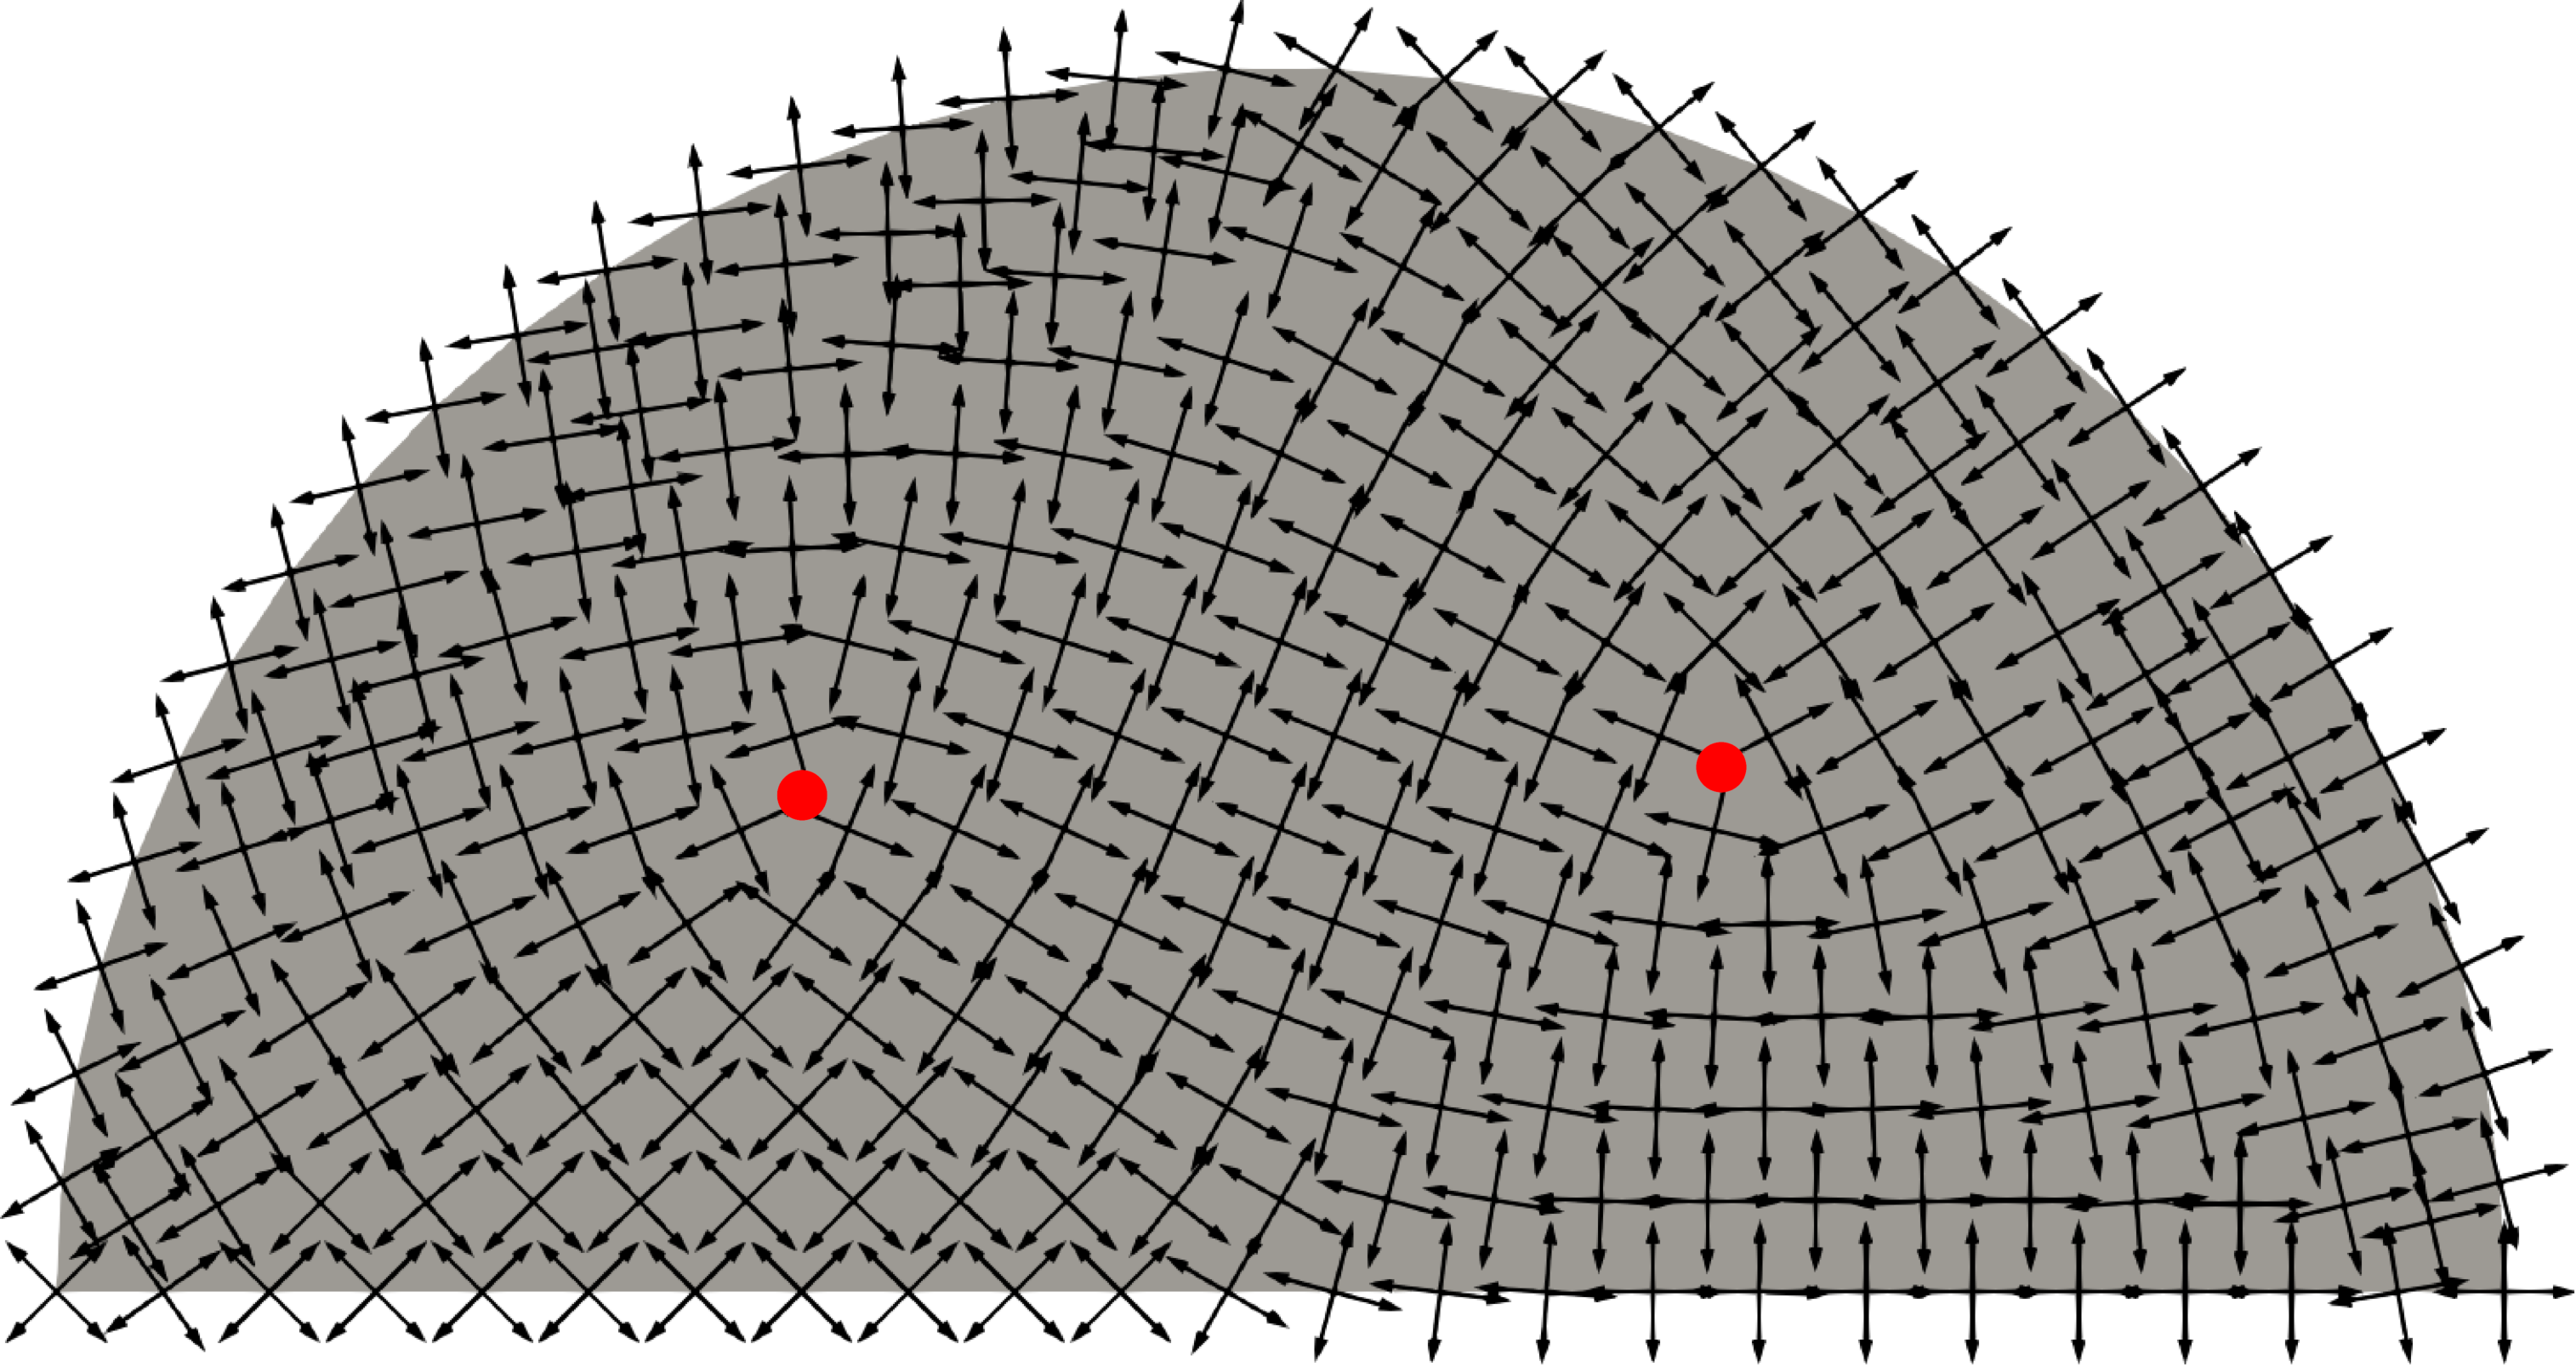
\includegraphics[scale=0.092]{images/mode_prop_cross_beam.pdf} \hspace{0.2cm}
        %\footnotesize Champ de croix
        }
\only<4>{
        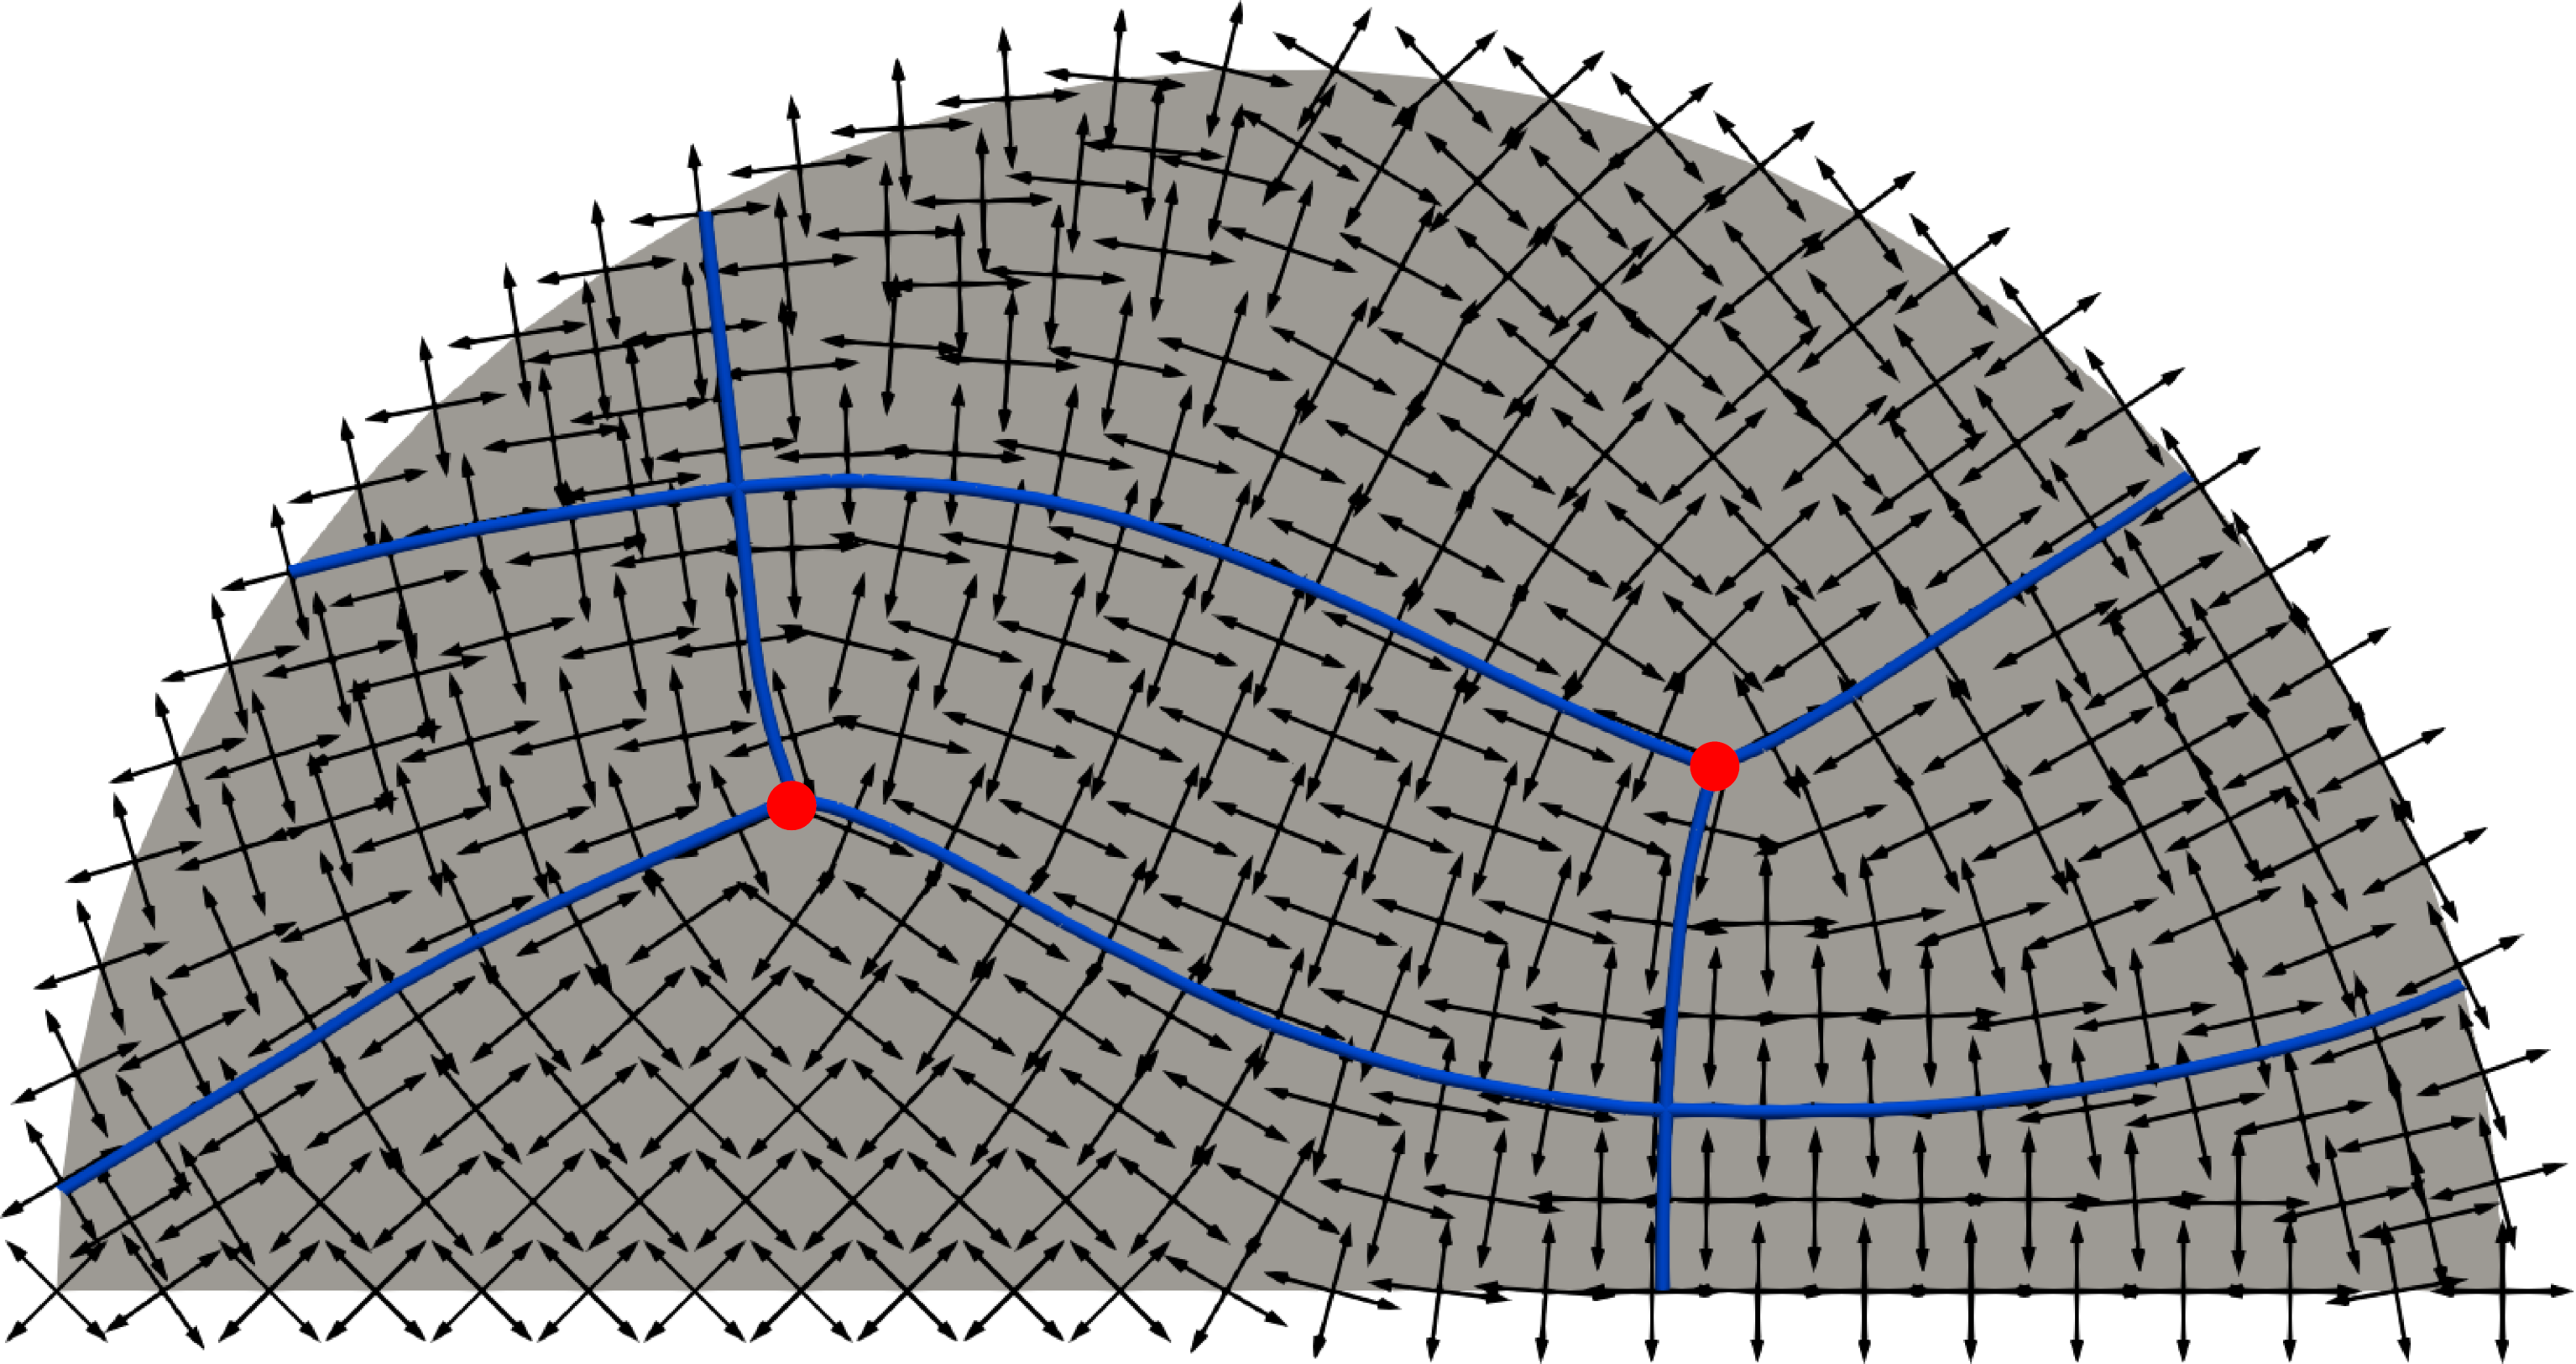
\includegraphics[scale=0.092]{images/mode_prop_stream_non_align_beam.pdf} \hspace{0.2cm}
        %\footnotesize Champ de croix
        }
        \end{column}
    \end{columns}

\end{frame}


%\begin{frame}{Prise en compte de champs de croix arbitraires}

%    \begin{columns}
%        \begin{column}{0.33\textwidth}
%        \centering
%\onslide<1->{
%        %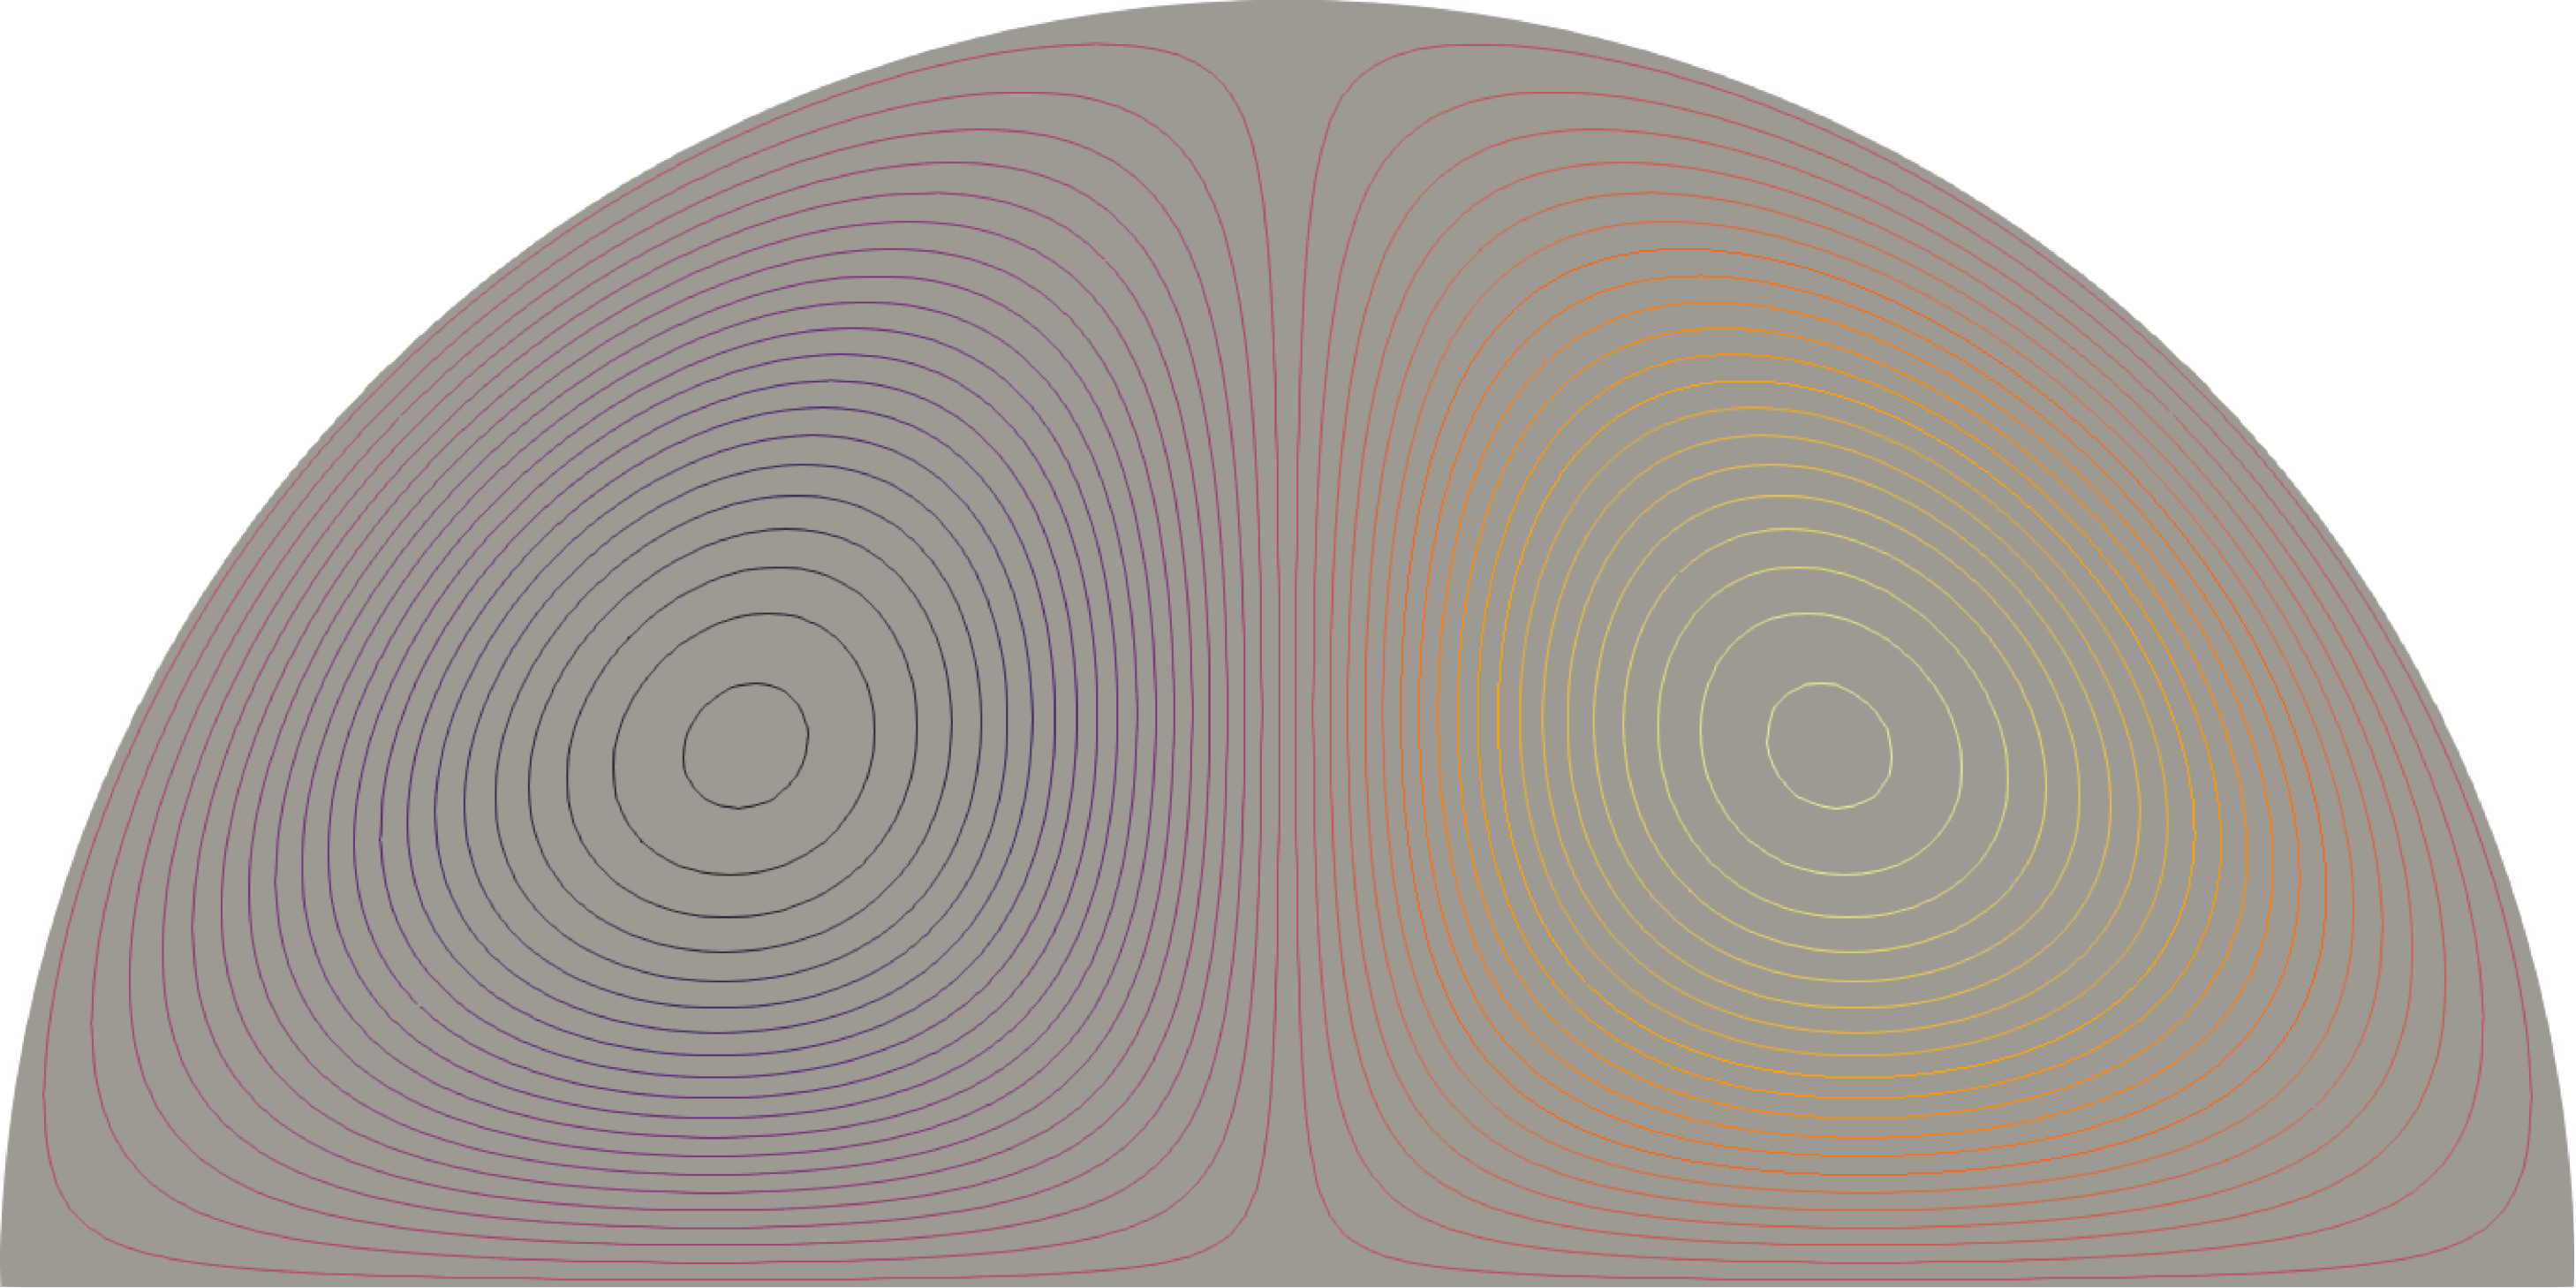
\includegraphics[scale=0.091]{images/mode_prop.pdf}
%        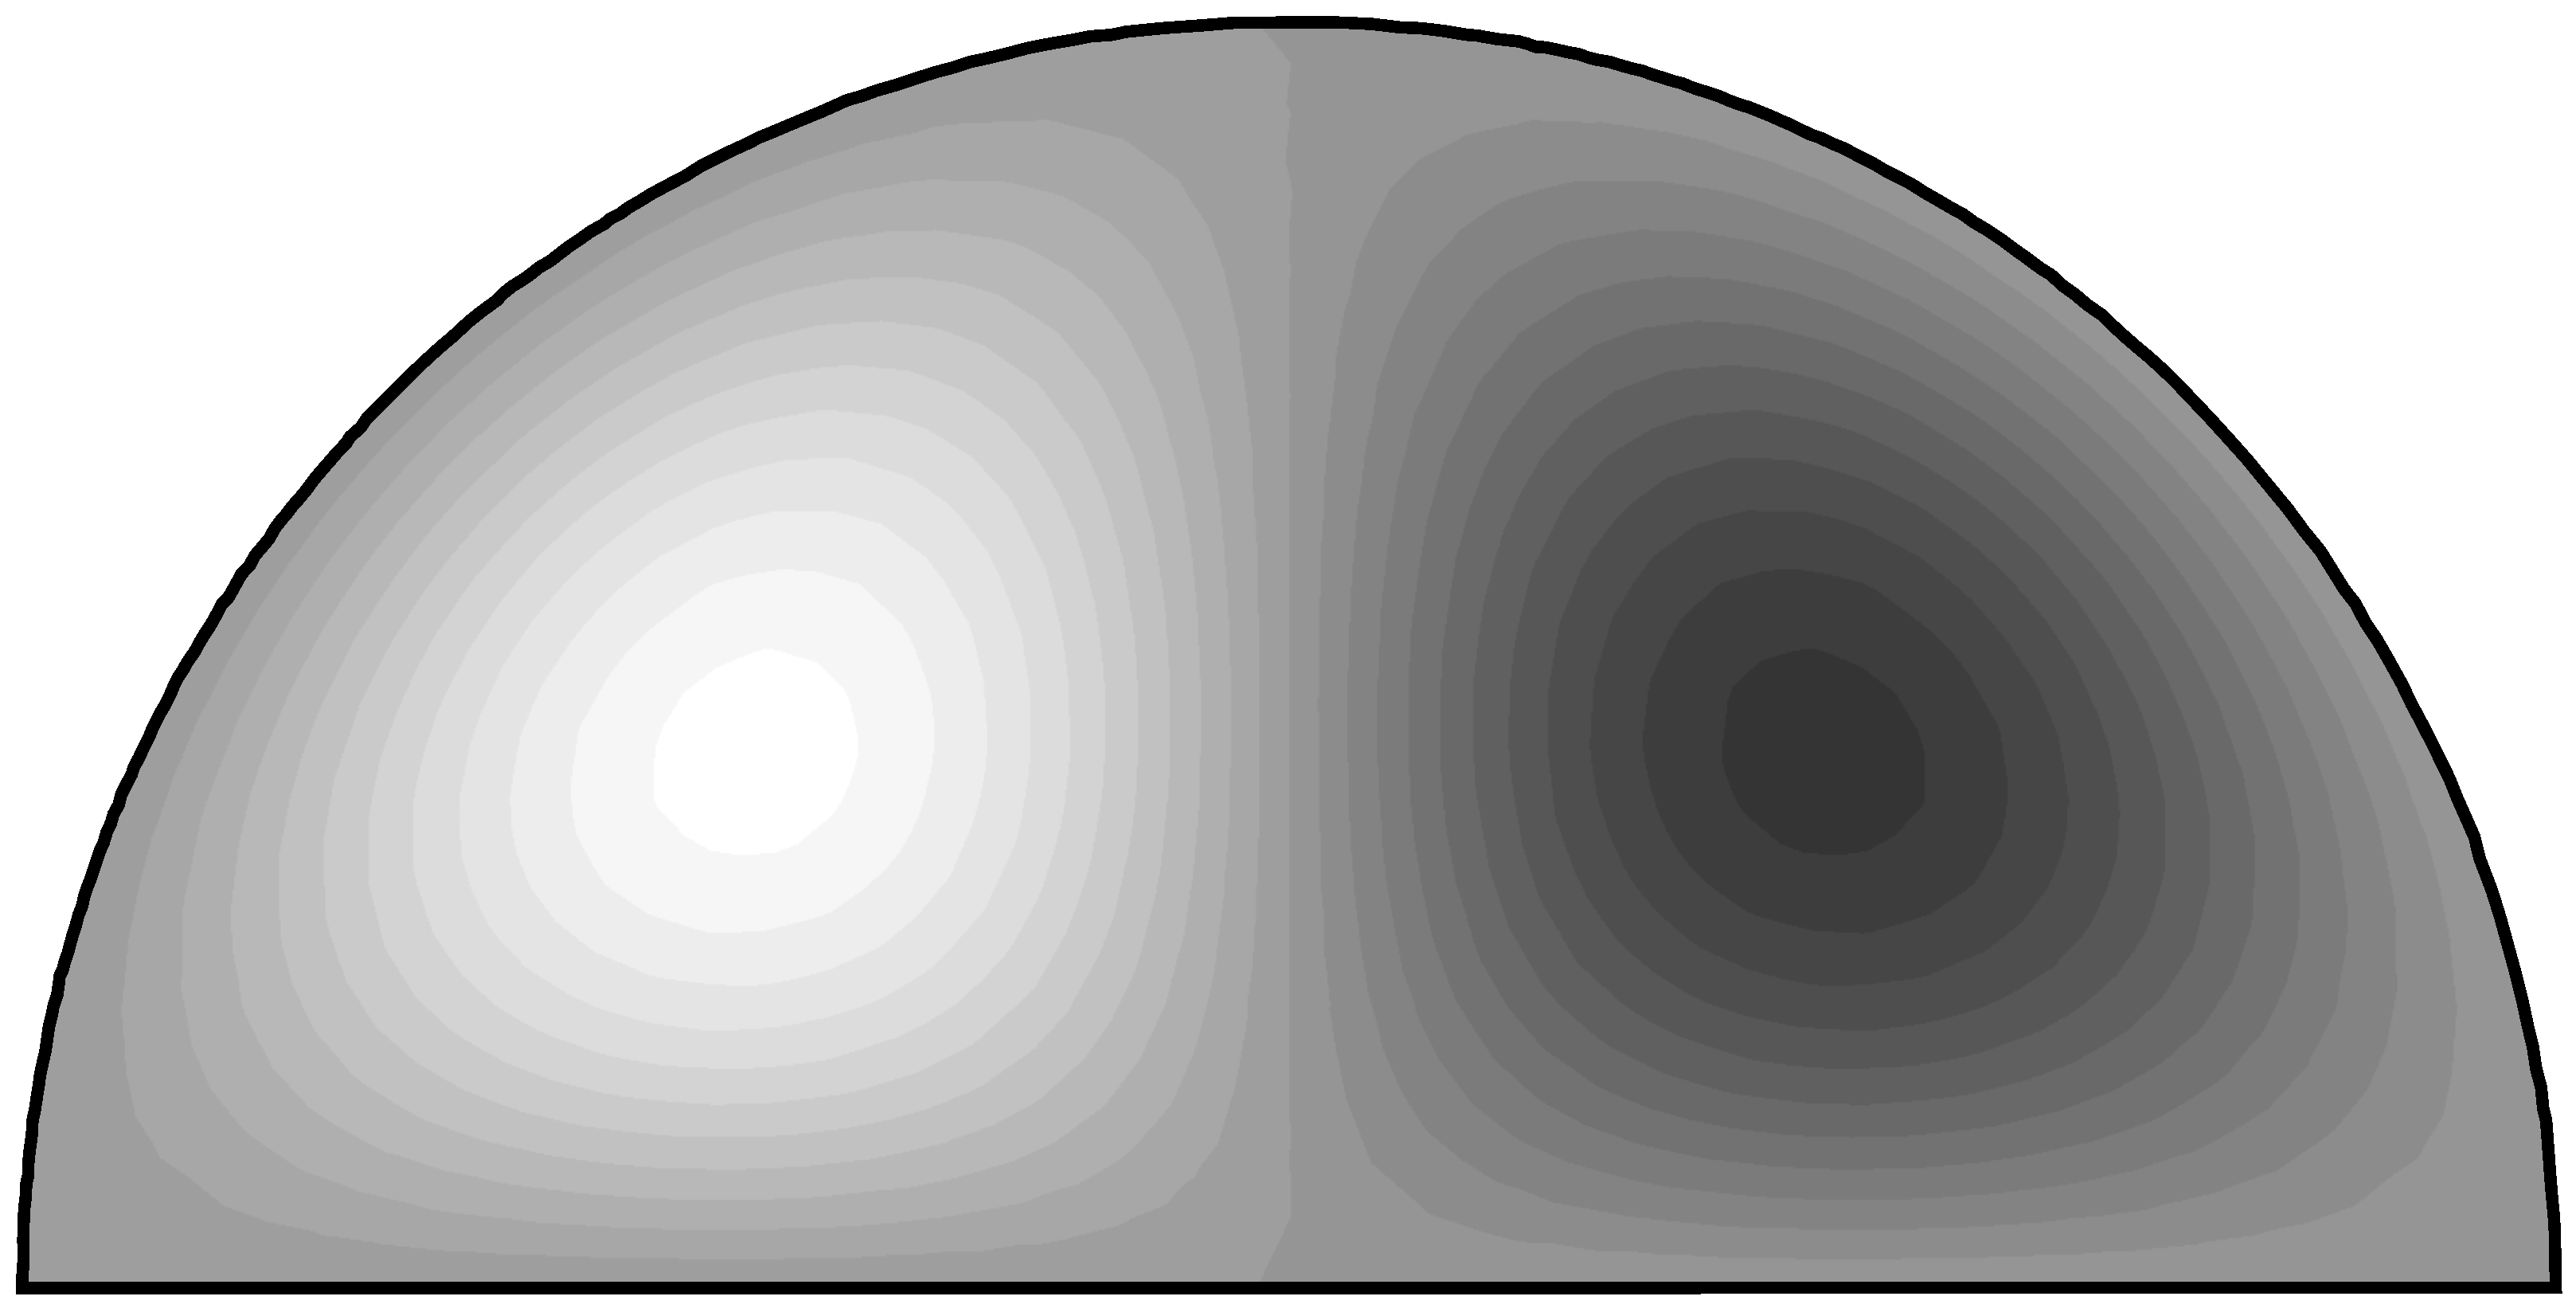
\includegraphics[scale=0.085]{images/demiDiscValProp.eps} \hspace{0.2cm}
%        \footnotesize Mode propre sur le demi-disque}
%        \end{column}
%        \begin{column}{0.33\textwidth}
%        \centering
%\onslide<2->{
%        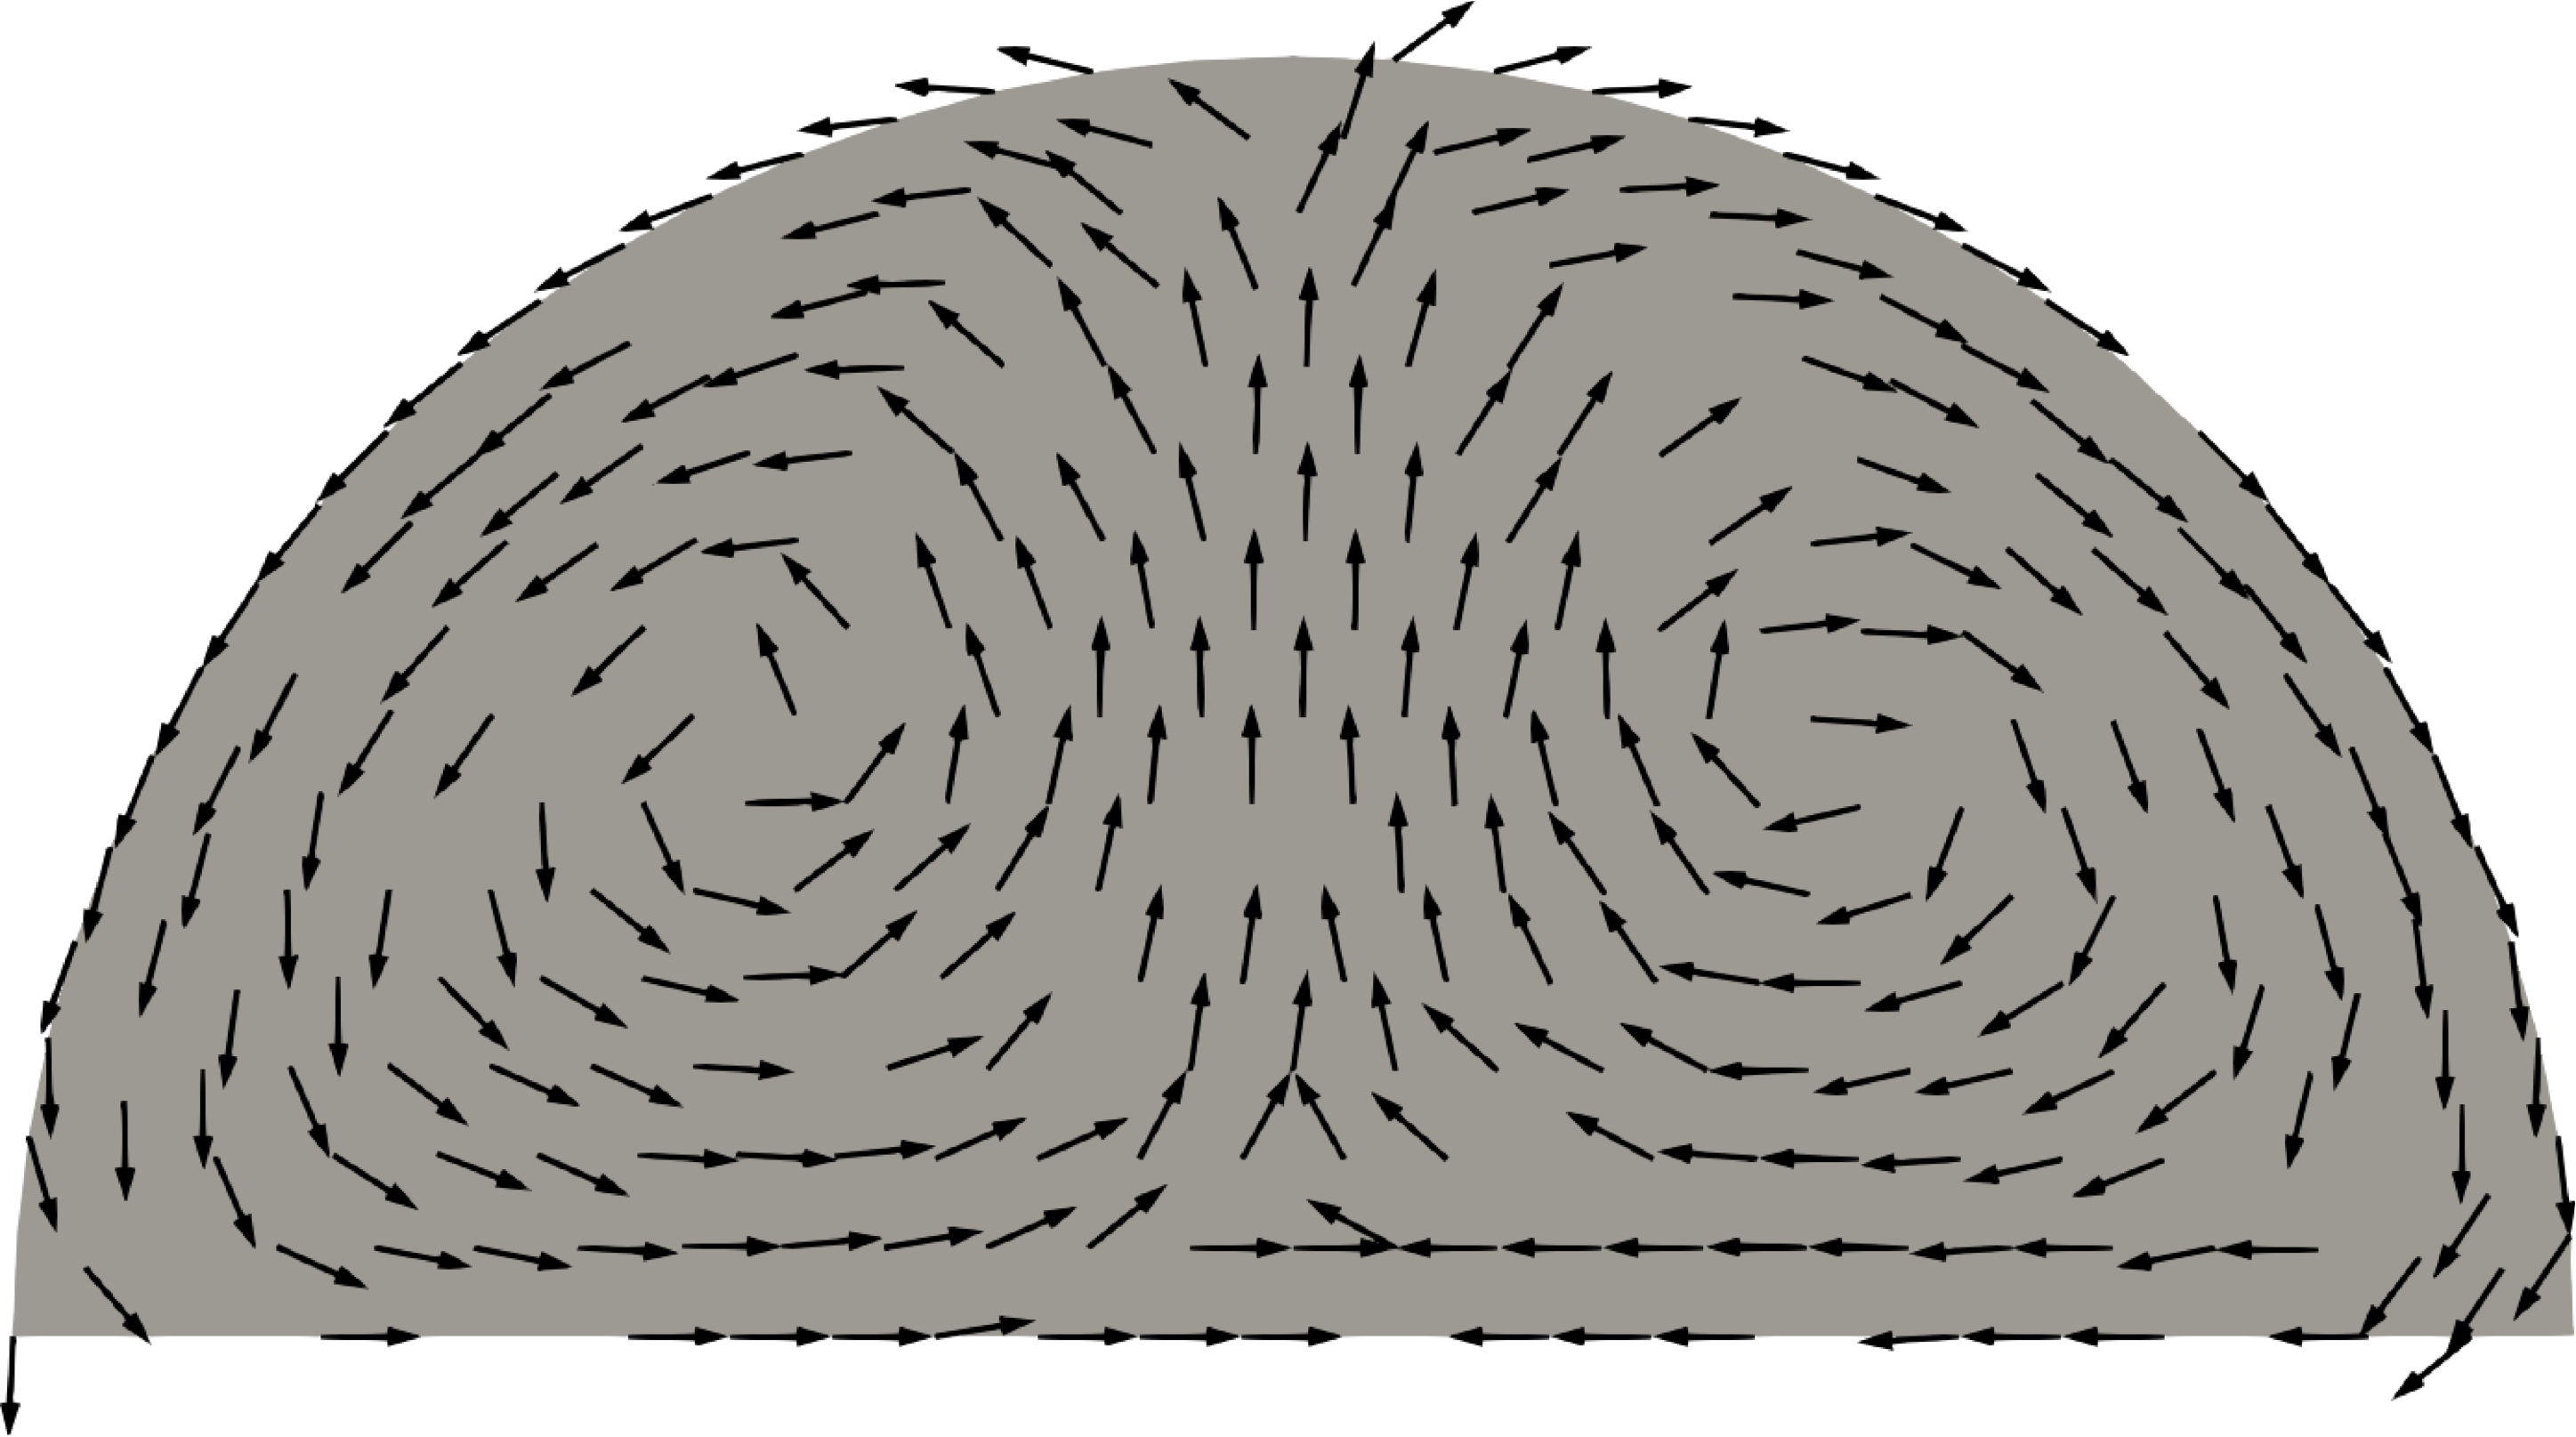
\includegraphics[scale=0.085]{images/iso_tangente.pdf} %\hspace{0.2cm}
%        \footnotesize Tangentes aux lignes de niveaux}
%        \end{column}
%        \begin{column}{0.33\textwidth}
%        \centering
%\onslide<3->{
%        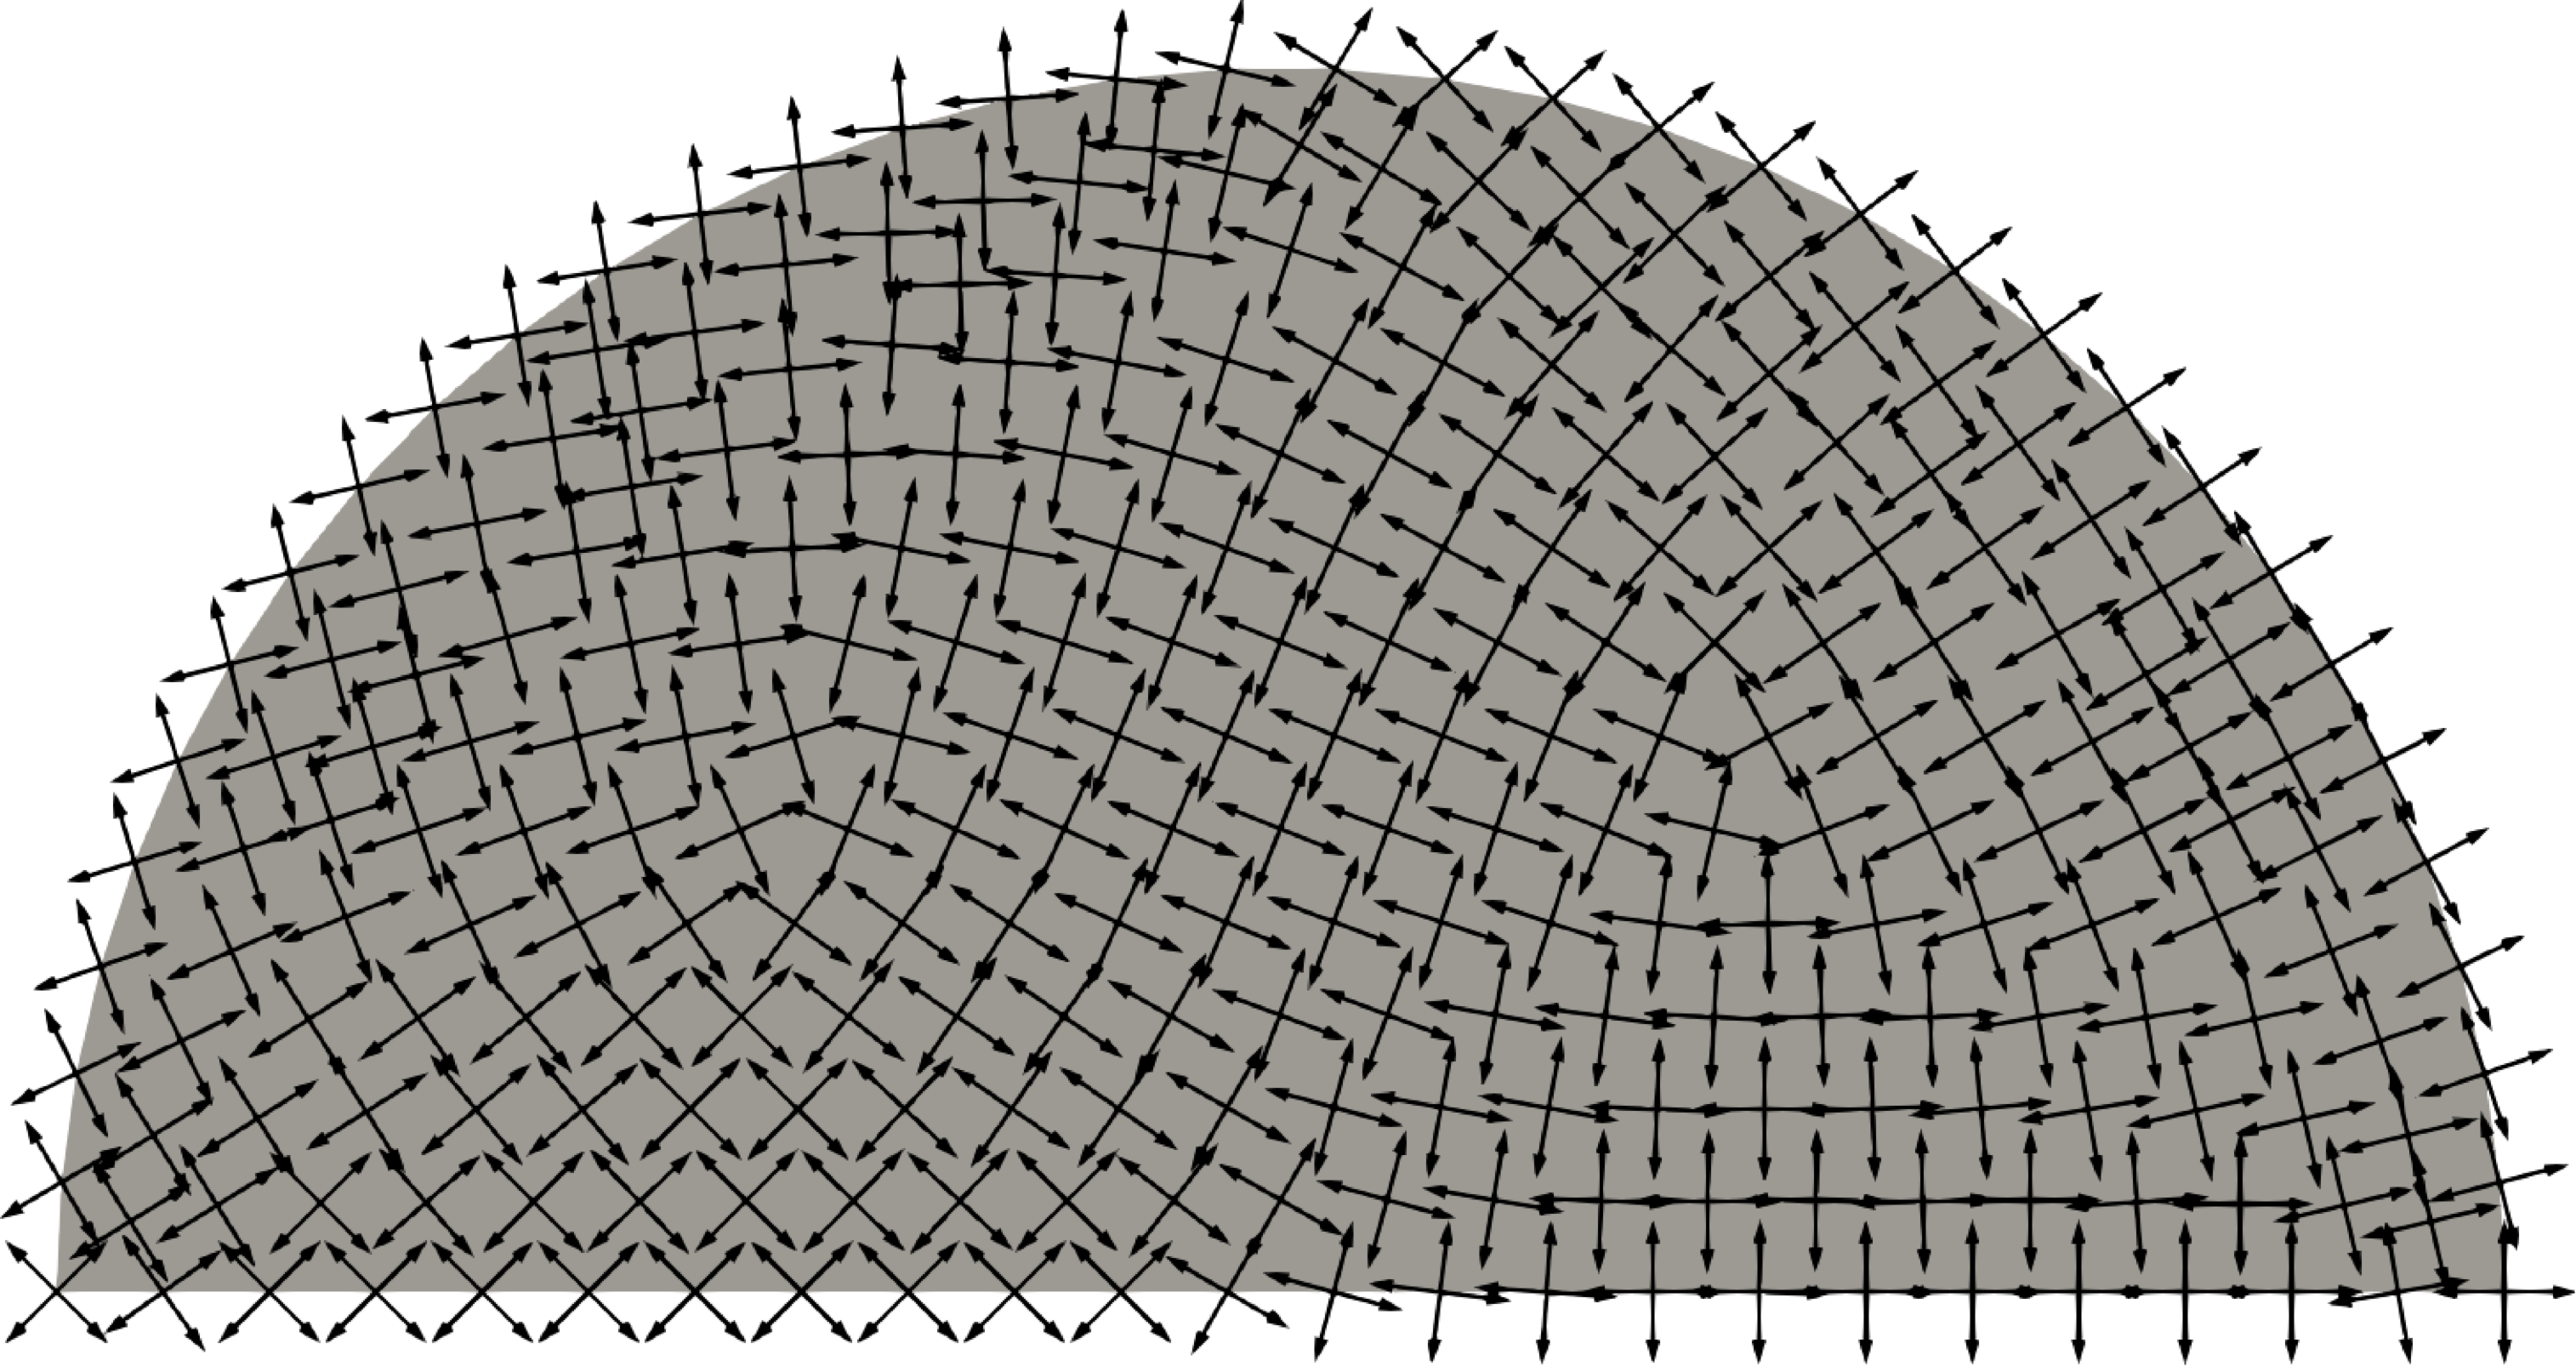
\includegraphics[scale=0.085]{images/mode_prop_cross.pdf} \hspace{0.2cm}
%        \footnotesize Champ de croix}
%        \end{column}
%    \end{columns}

%    \begin{columns}
%\onslide<5->{
%        \begin{column}{0.5\textwidth}

%        \begin{itemize}
%            \item Comment montrer q'une partition donnée est de quatres côtés ?\\\vspace{0.2cm}
%            \item Analyse du comportement locale du champ aux voisinnages de points singuliers.\\\vspace{0.2cm}
%            %\item Exemples%\\\vspace{0.2cm}
%        \end{itemize}
%}
%    \vspace{0.5cm}
%        \end{column}
%        \begin{column}{0.5\textwidth}
%             \centering
%\onslide<4->{
%            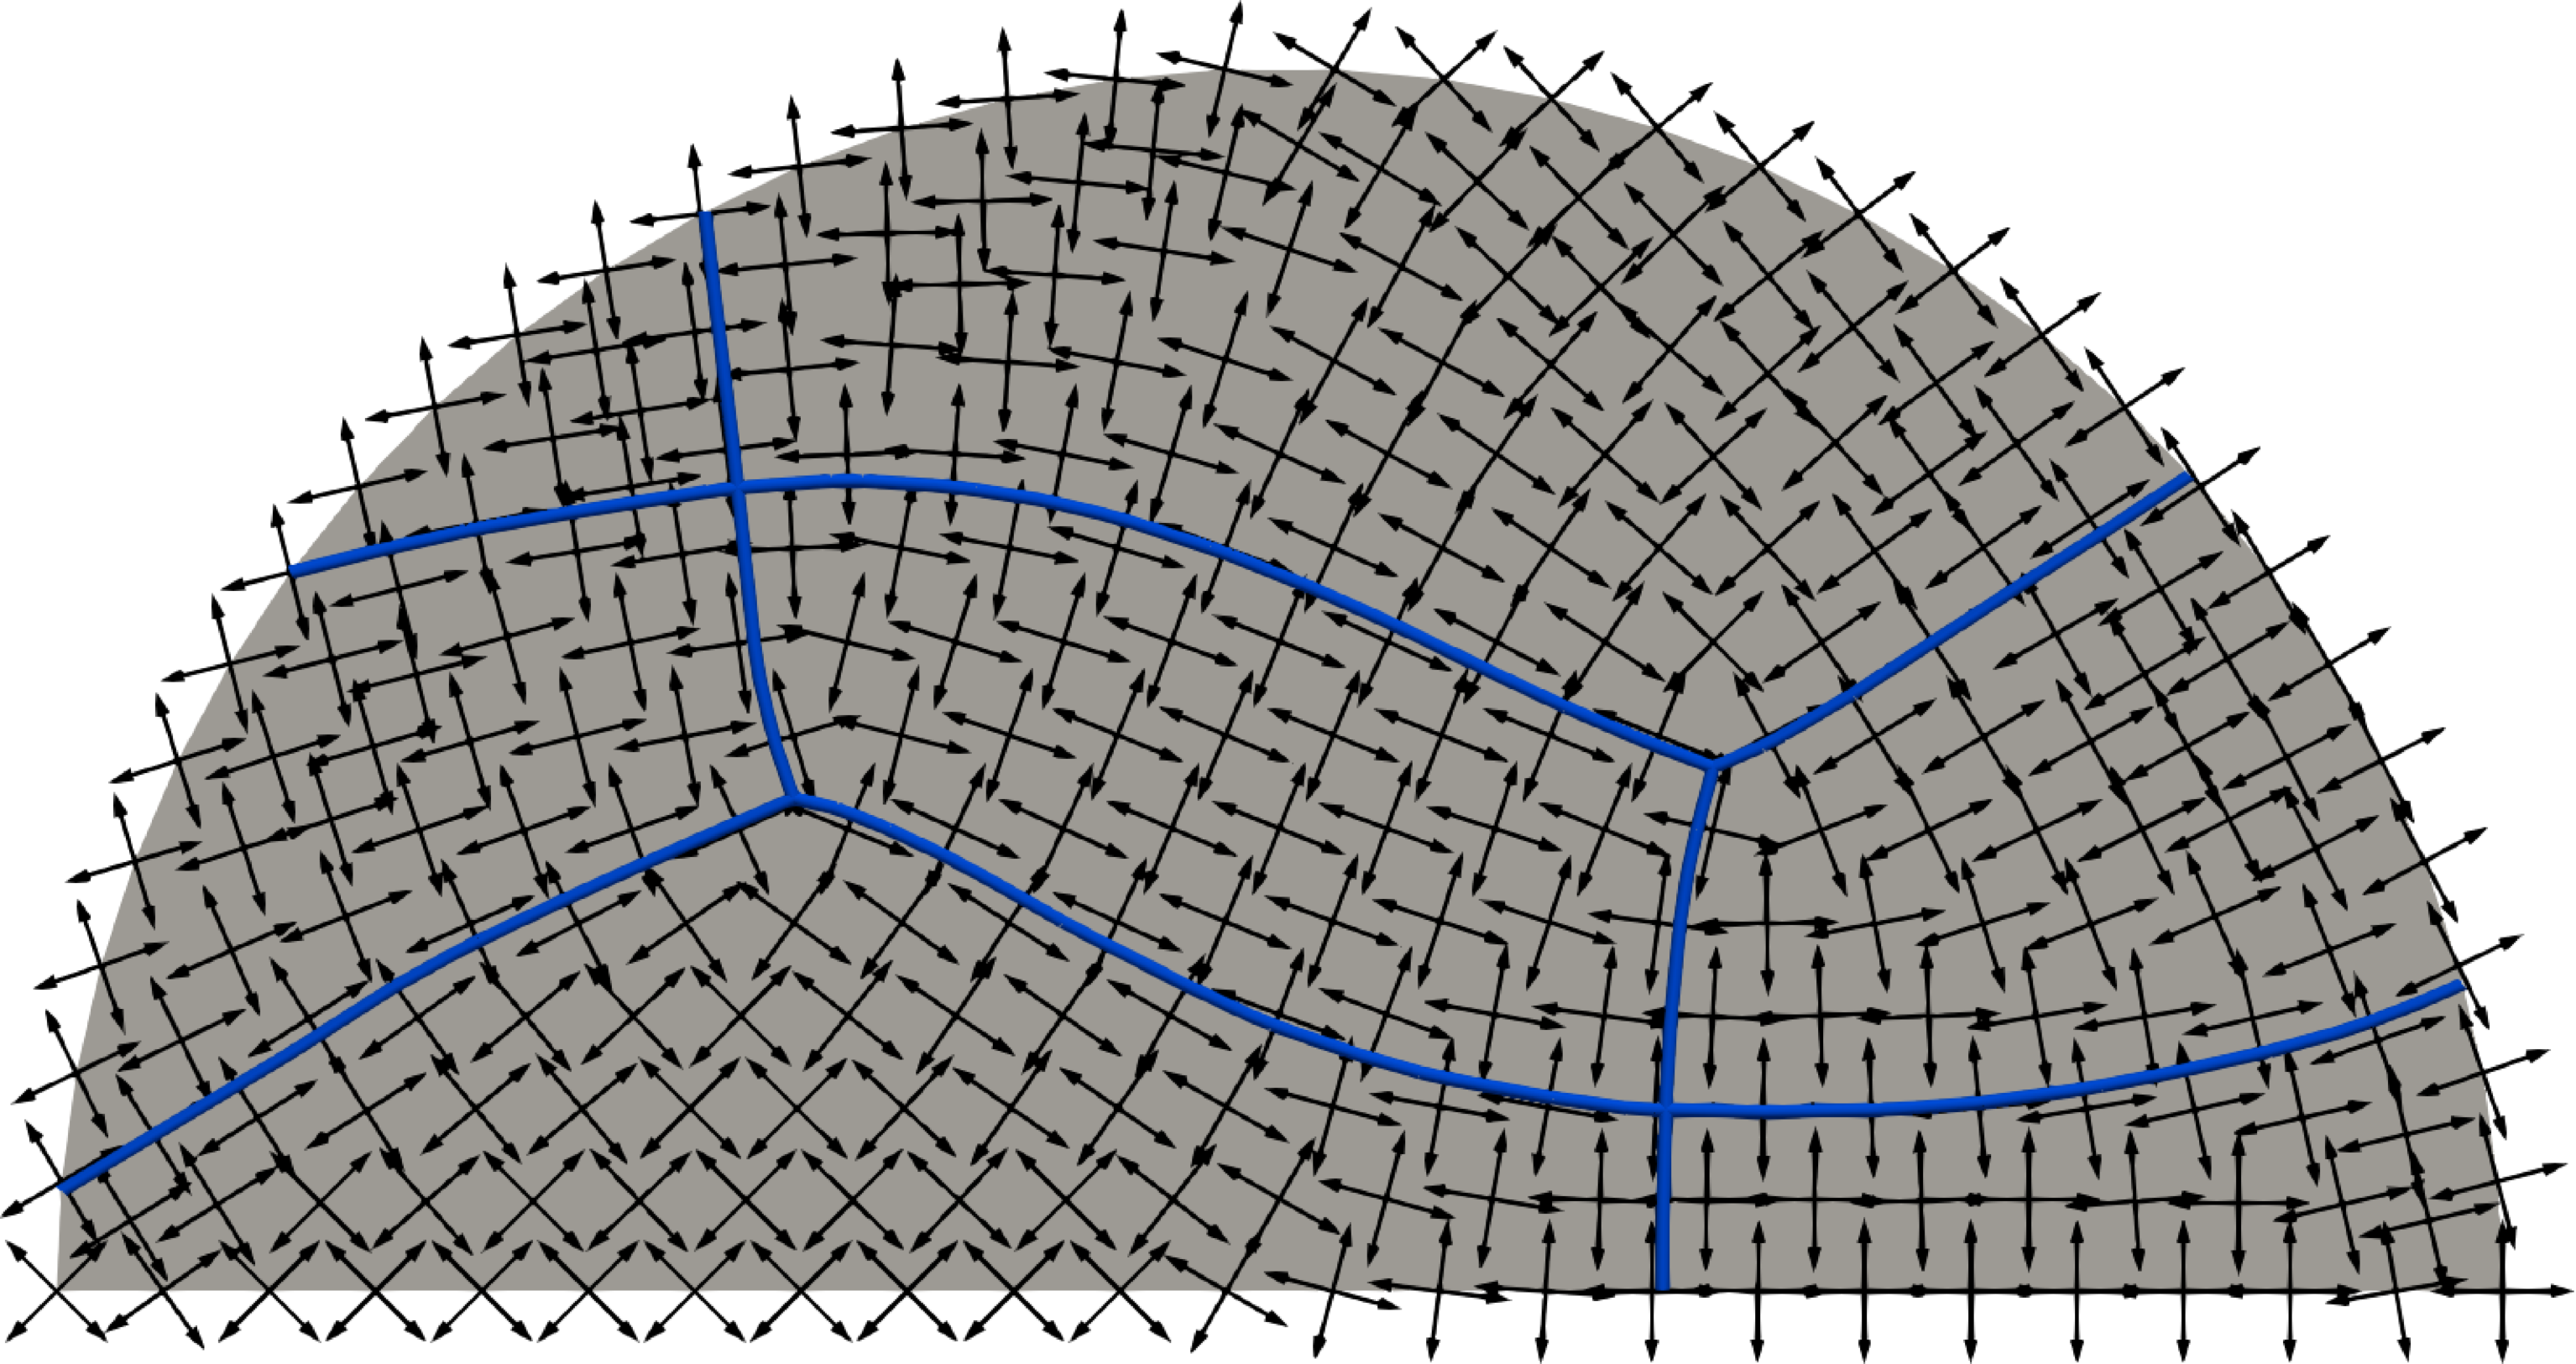
\includegraphics[scale=0.125]{images/mode_prop_stream_non_align.pdf}
%        }
%            %\hspace{0.2cm}
%            %\caption{\footnotesize Partitionnement}
%            \vspace{0.5cm}
%        \end{column}
%    \end{columns}
%\end{frame}

\begin{frame}{Prise en compte de champs de croix arbitraires}%{Comment }
\small
\vspace{-0.2cm}
  \begin{columns}
    \begin{column}{0.7\textwidth}
{\bf Qu'est ce qu'une partition de quatres côtés ?}\\\vspace{0.2cm}
    {\color{onera} Index:} nombre d'enroulement du champ autour d'un point
\begin{itemize}
    \item si $p\in\Omega$ alors $id_{\bar{u}}(p) = \frac{1}{2\pi}\int_\gamma d\theta_{\bar{u}}$
    \item si $p\in\partial\Omega$ alors $id^\partial_{\bar{u}}(p)=\frac{1}{2\pi}\left[\pi-\hat{p}+\lim\limits_{s\rightarrow 0}\int_s^{1-s}d\theta_{\bar{u}}^\gamma\right]$
\end{itemize}
{\color{onera} Valence:} nombre de séparatrices associé à un point
\begin{itemize}
    \item si $p\in\Omega$ alors $N_s(p) = 4-4id_{\bar{u}}(p)$
    \item si $p\in\partial\Omega$ alors $N_s(p) = 3-4id^\partial_{\bar{u}}(p)$
\end{itemize}
{\bf Exemple:} (Voir figure)\\\vspace{0.1cm}
\begin{onerablock}[drop fuzzy shadow]{\small  Lemme}
    \small L'index de bord d'un point (singulier ou d'intersection) par rapport à une partition $\mathcal{P}$ donnée est 1/4.
\end{onerablock}
    \end{column}
    \begin{column}{0.3\textwidth}
        \centering
  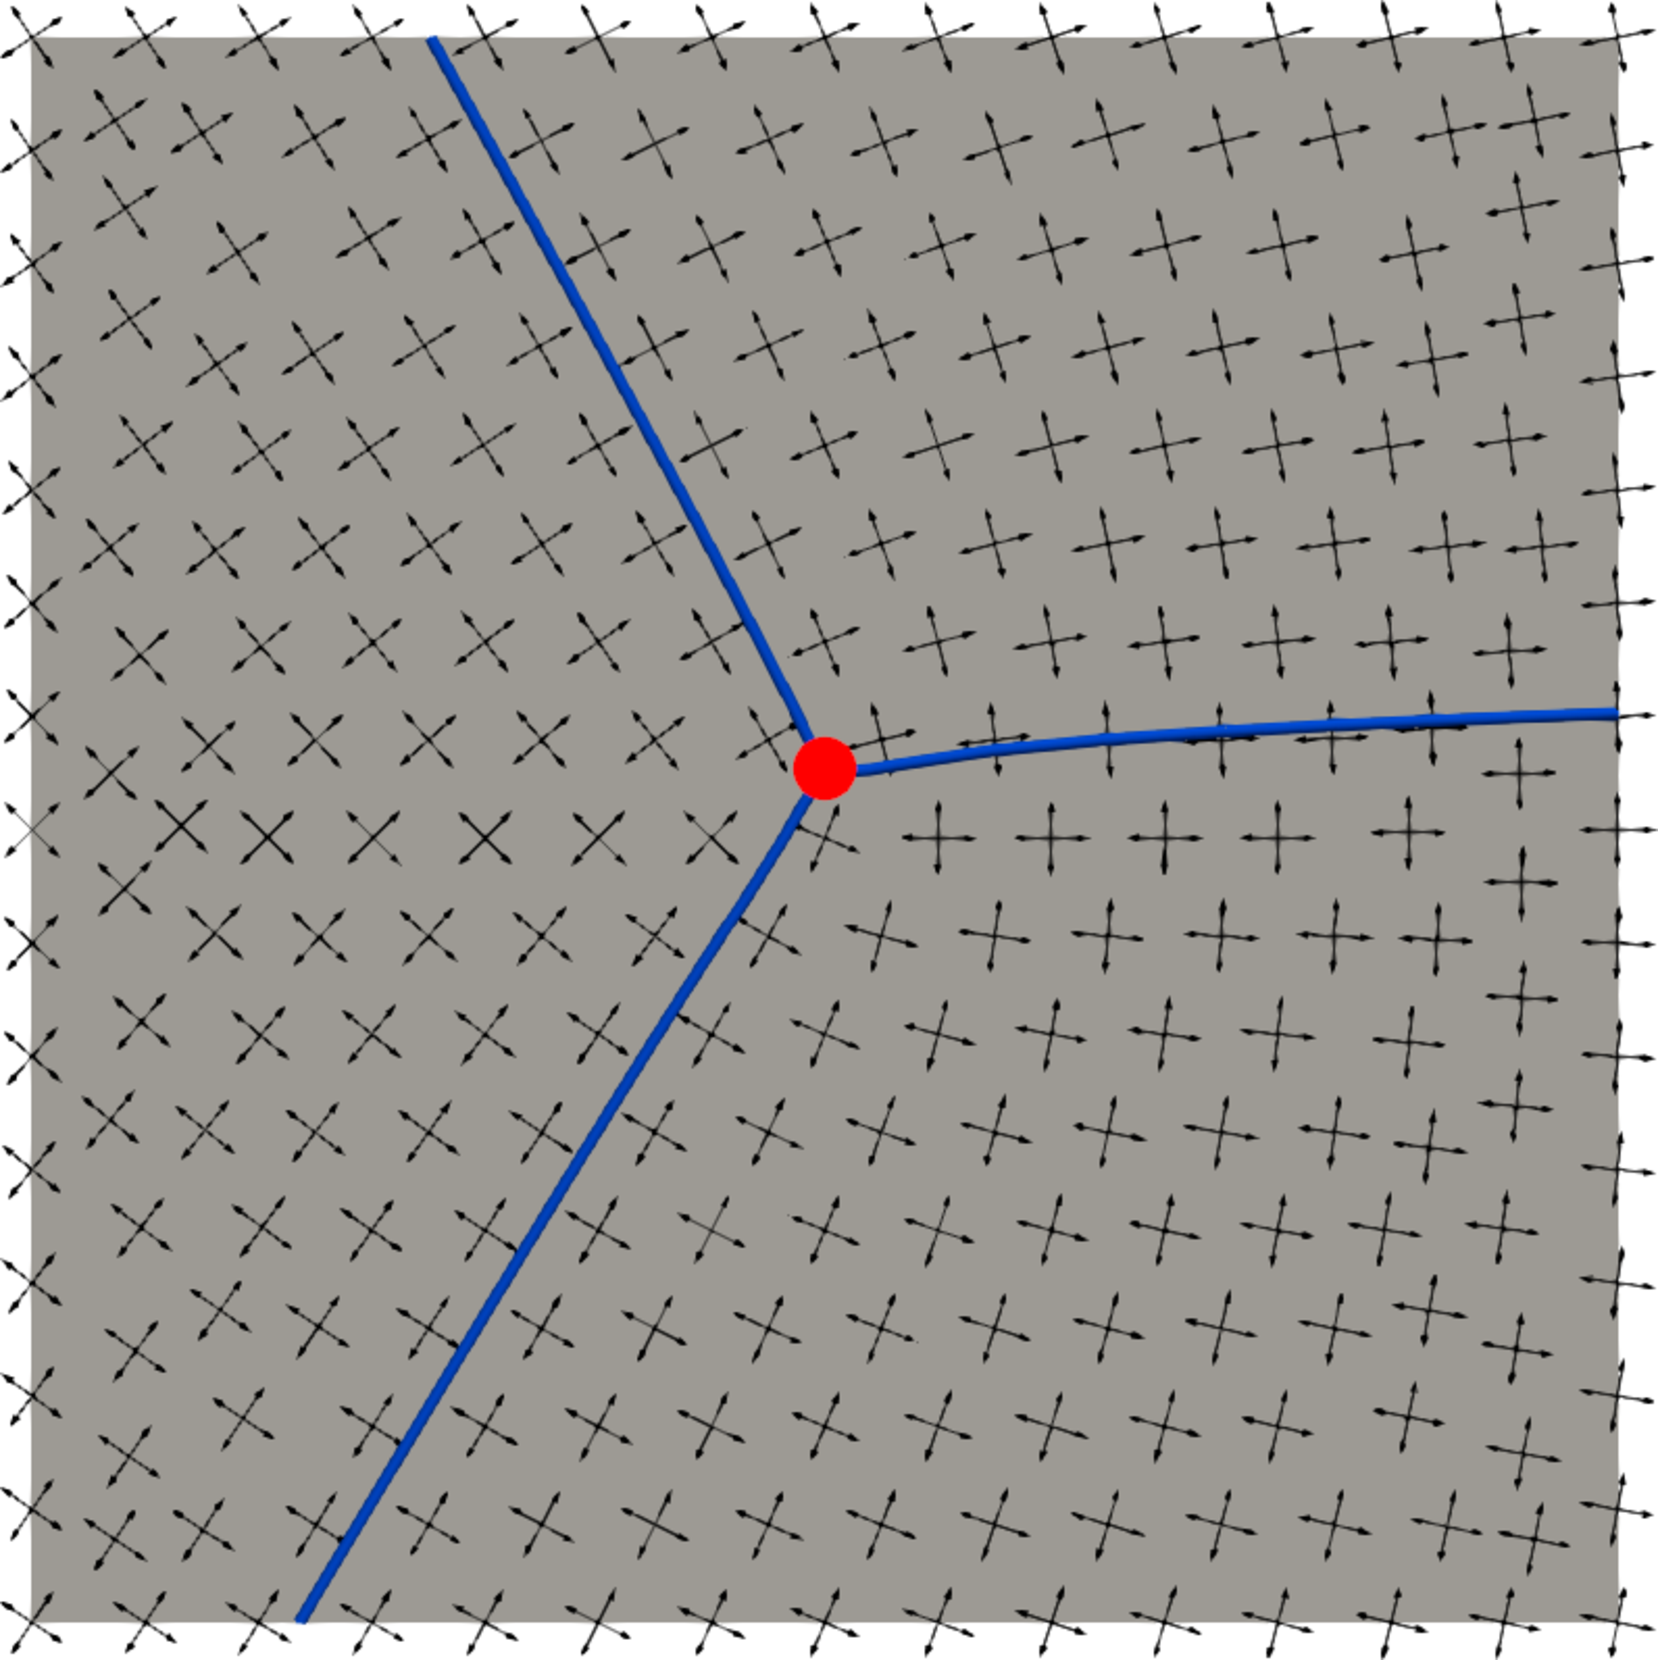
\includegraphics[scale=0.1]{images/sepa_3.pdf}
  \scriptsize $id_{\bar{u}}(p)=1/4, N_s(p) = 3$
  \\\vspace{0.1cm}
  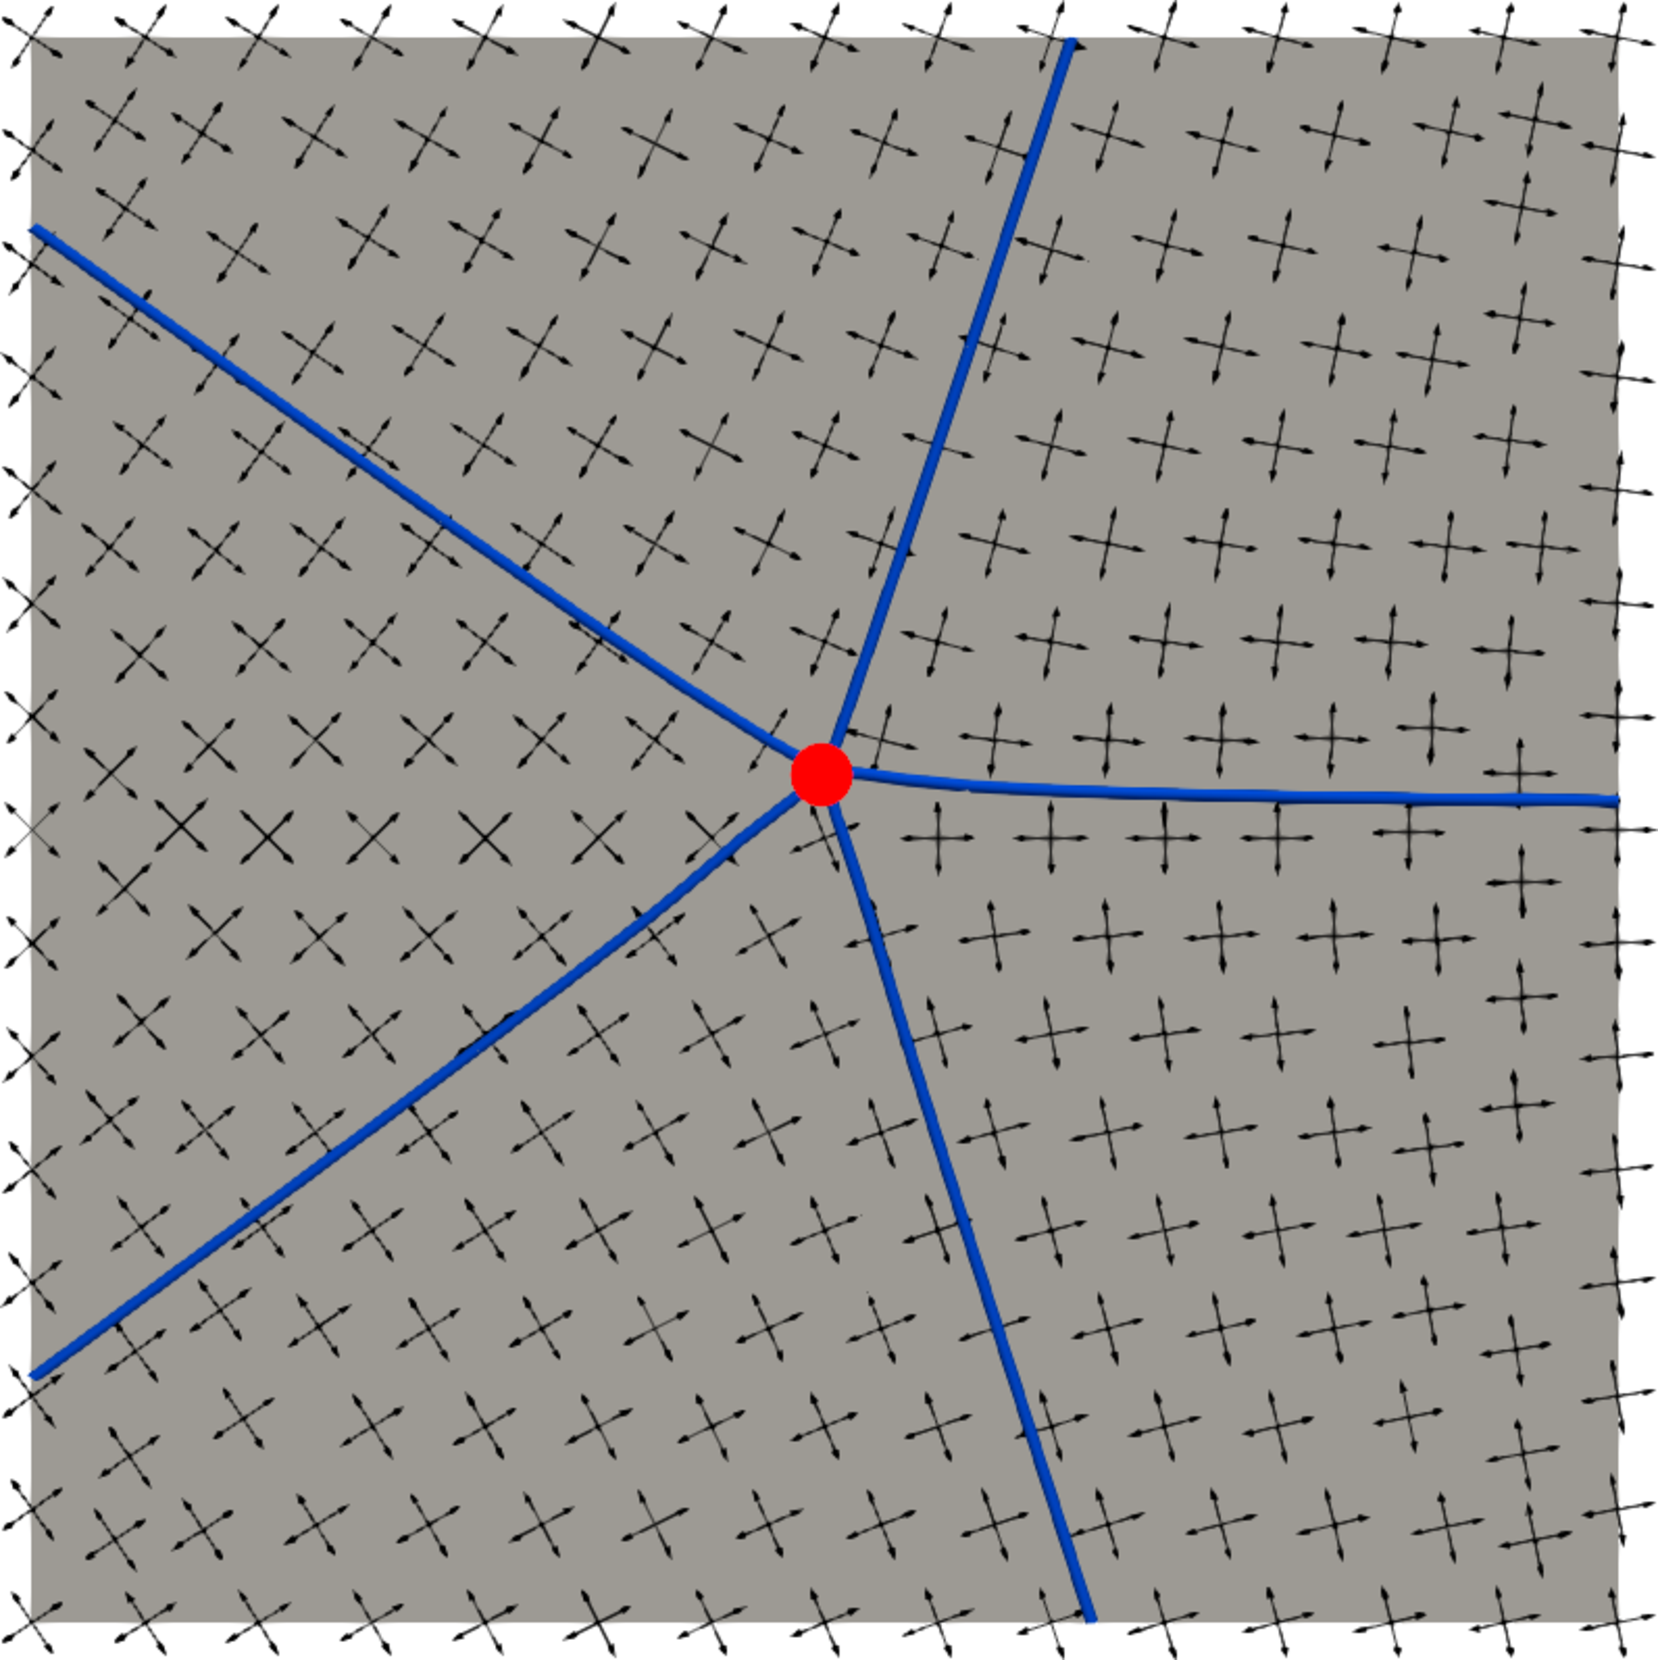
\includegraphics[scale=0.1]{images/sepa_5.pdf}
  \scriptsize $id_{\bar{u}}(p)=-1/4, N_s(p) = 5$
  \\\vspace{0.3cm}
    \end{column}
\end{columns}

\end{frame}

\begin{frame}{Prise en compte de champs de croix arbitraires}%{Comment }
\small
%{\bf Qu'est ce qu'une partition de quatres côtés ?}\\
\vspace{-0.2cm}
On exploite ce résultat de la manière suivante: {\color{onera_gray} (formation des partition de 4 côtés)}\\\vspace{0.1cm}
 Soit $\mathcal{P}$ une partition quelconque. {\color{onera_gray} (A cette étape on ne connait pas encore son nombre côtés, séparatrice à l'aveugle)}
$$\chi(\mathcal{P})=1. \quad\quad{\color{onera_gray} (\chi=2-2g-b, g=0, b=1)}$$
Par construction, les bords de la partition sont aligné avec le champ et elle ne contient pas de points singulier interne). Le théorème de Poincaré-Hopf donne alors:
$$\chi(\mathcal{P})=\sum_{i=1}^{n_c}id_{\bar{u}}(c_i).$$
Par combinaison, on obtient:
$$1=\sum_{i=1}^{n_c}\frac{1}{4}\Longrightarrow n_c=4.$$
\textbf{Conclusion :} Toute partition dont le bord est aligné avec le champ (séparatrices) aura 4 côtés.
\vspace{0.4cm}
\end{frame}



\begin{frame}{Prise en compte de champs de croix arbitraires}{Un exemple de champ de croix alignés sur le bord du domaine}

    \begin{columns}
        \begin{column}{0.33\textwidth}
        \centering
        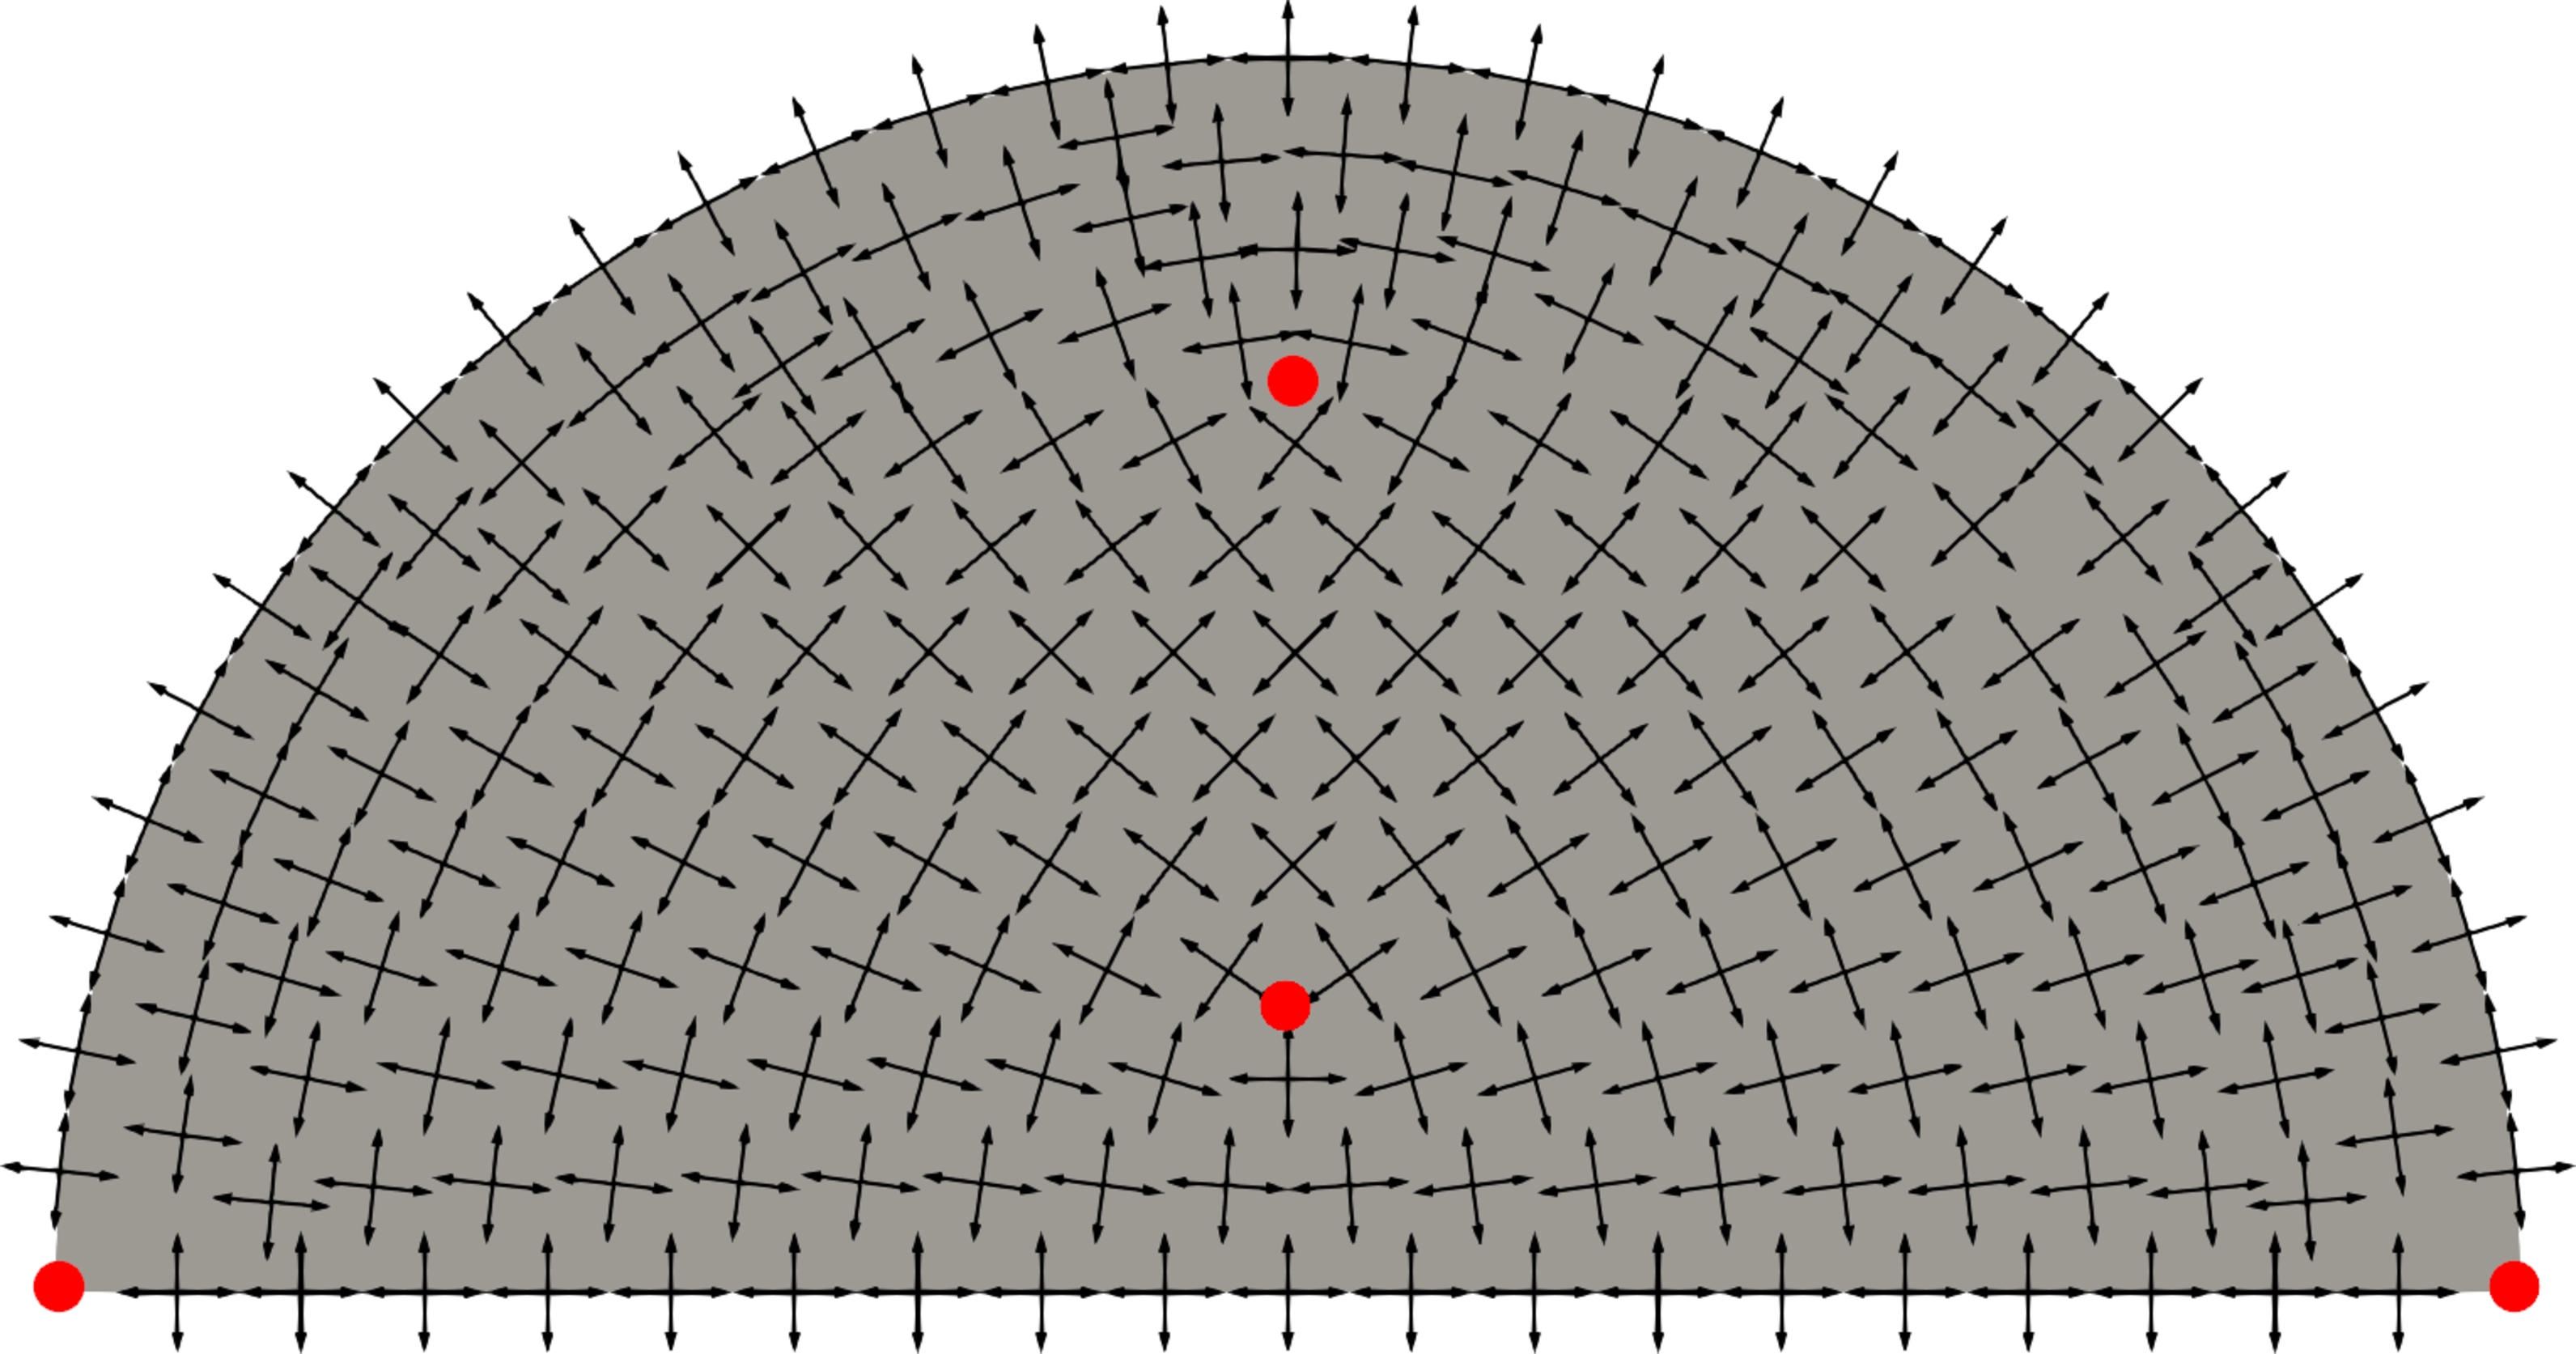
\includegraphics[scale=0.087]{images/demi_disc_align_first.pdf} \hspace{0.2cm}
        \footnotesize Champ de croix
        \end{column}
        \begin{column}{0.33\textwidth}
        \centering
        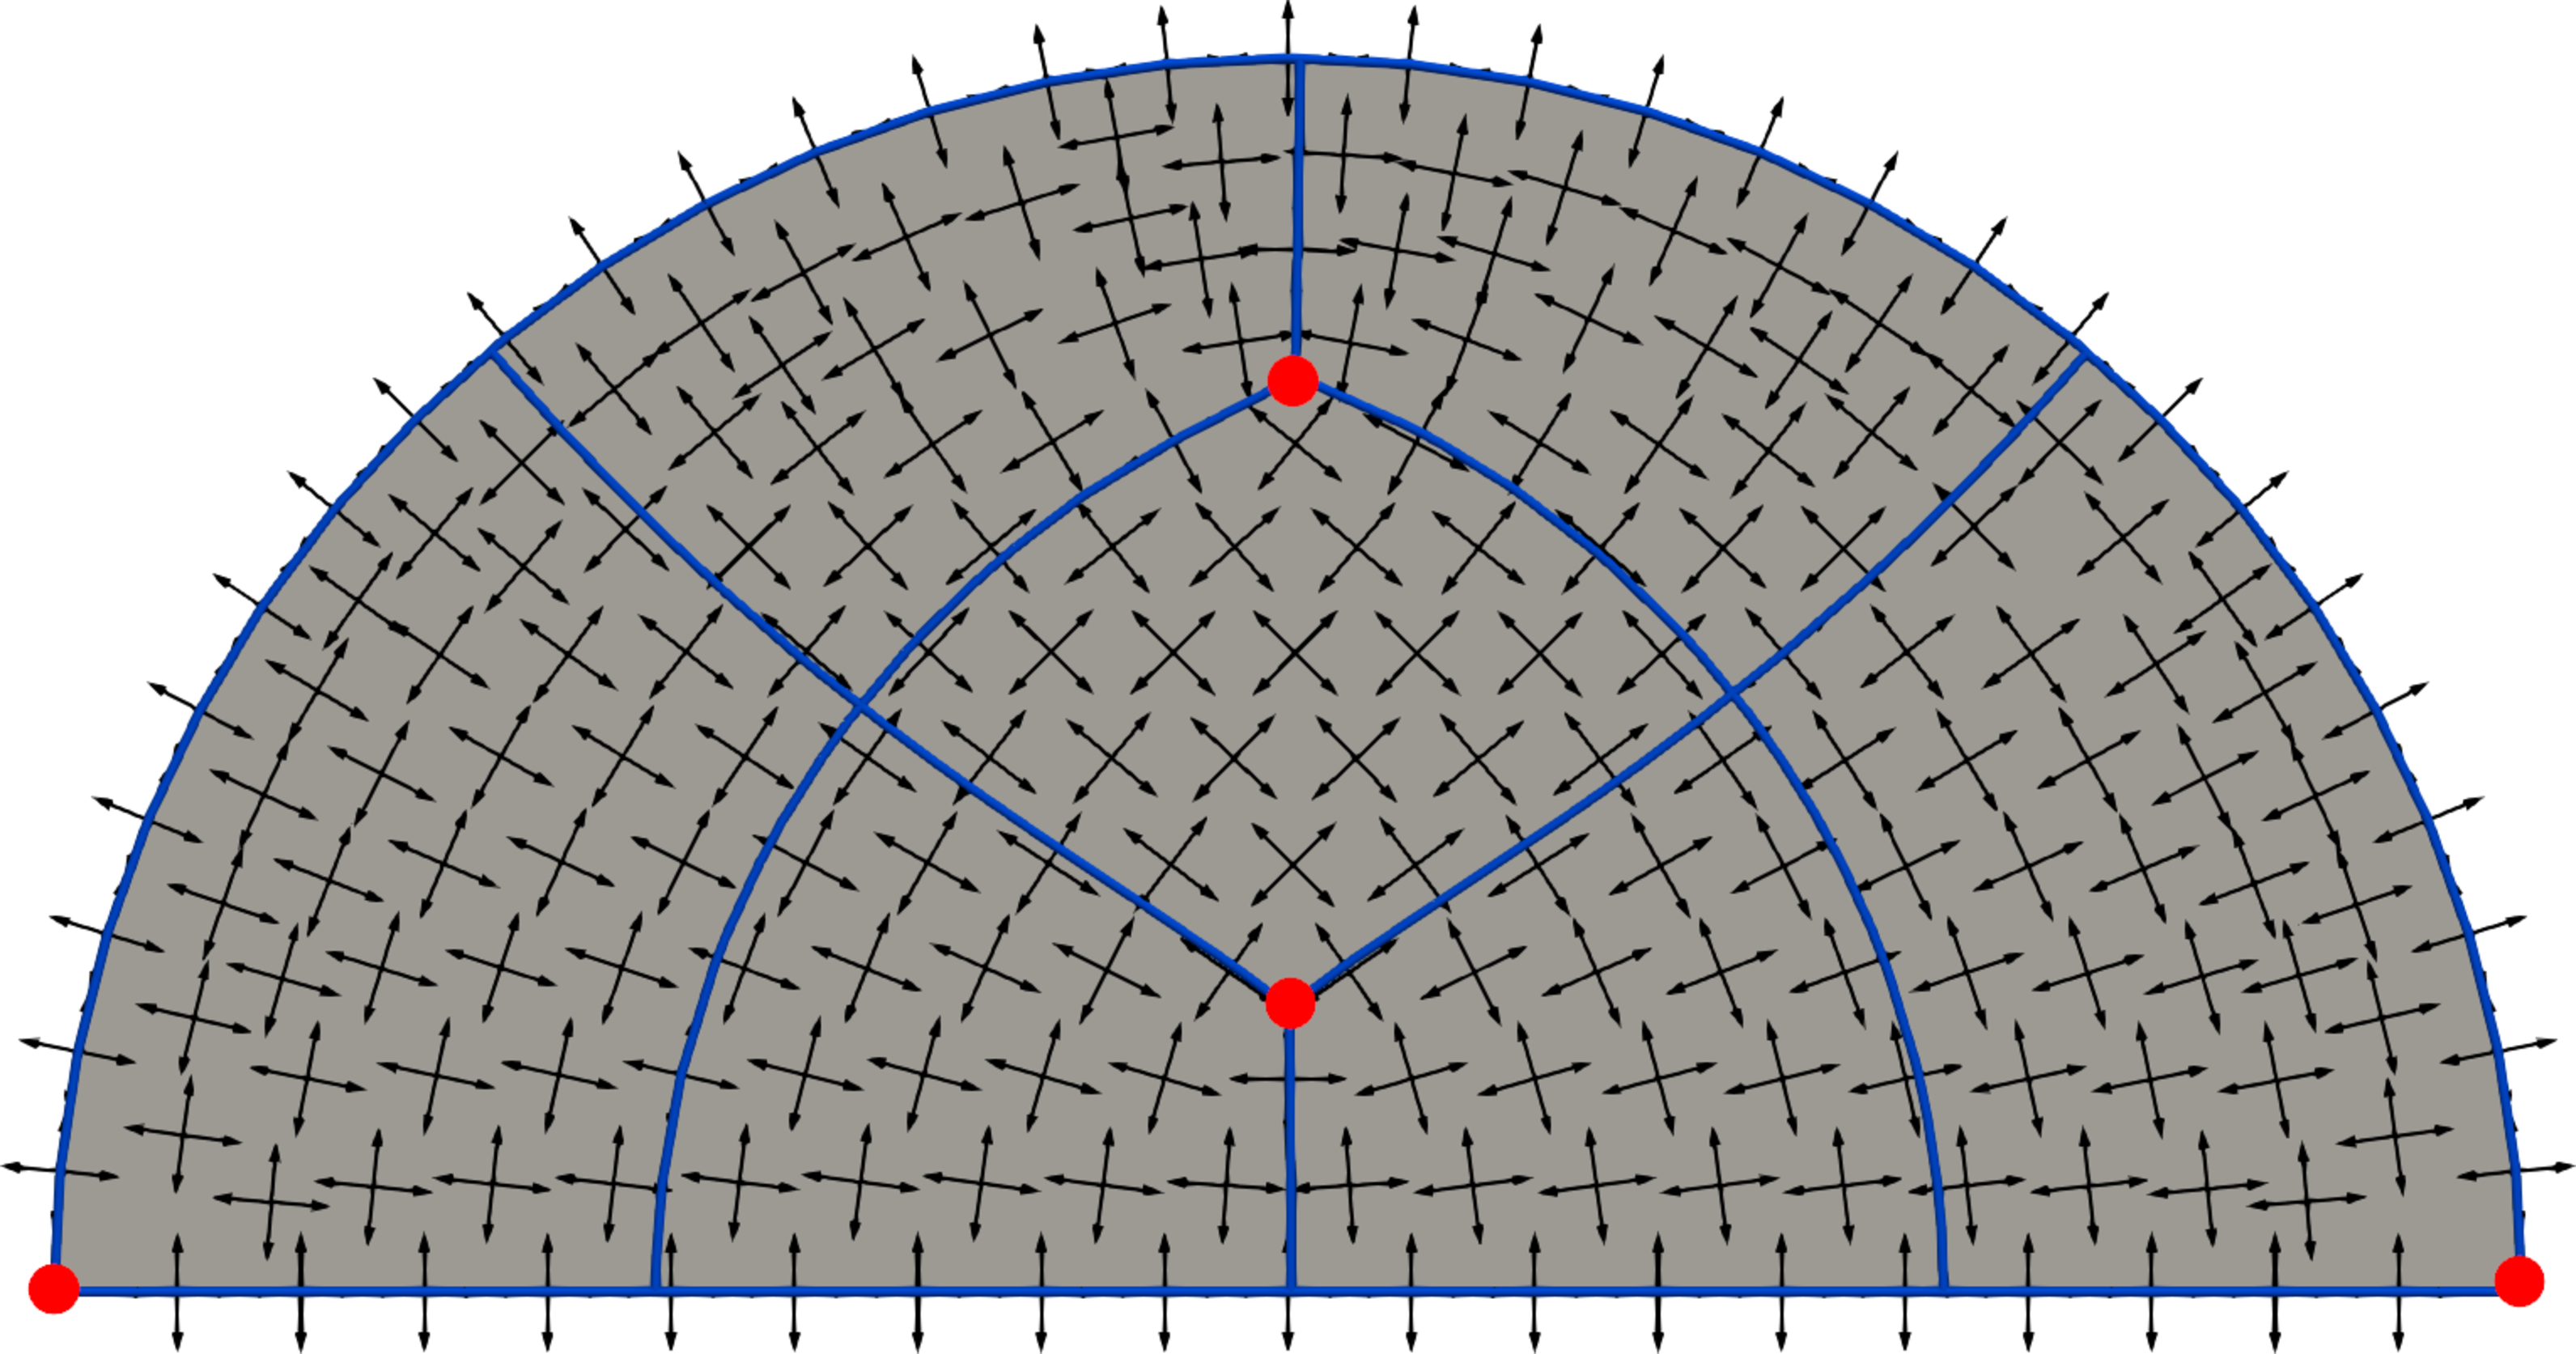
\includegraphics[scale=0.087]{images/demi_disc_align_second.pdf} \hspace{0.2cm}
        \footnotesize Partitionnement
        \end{column}
        \begin{column}{0.33\textwidth}
        \centering
        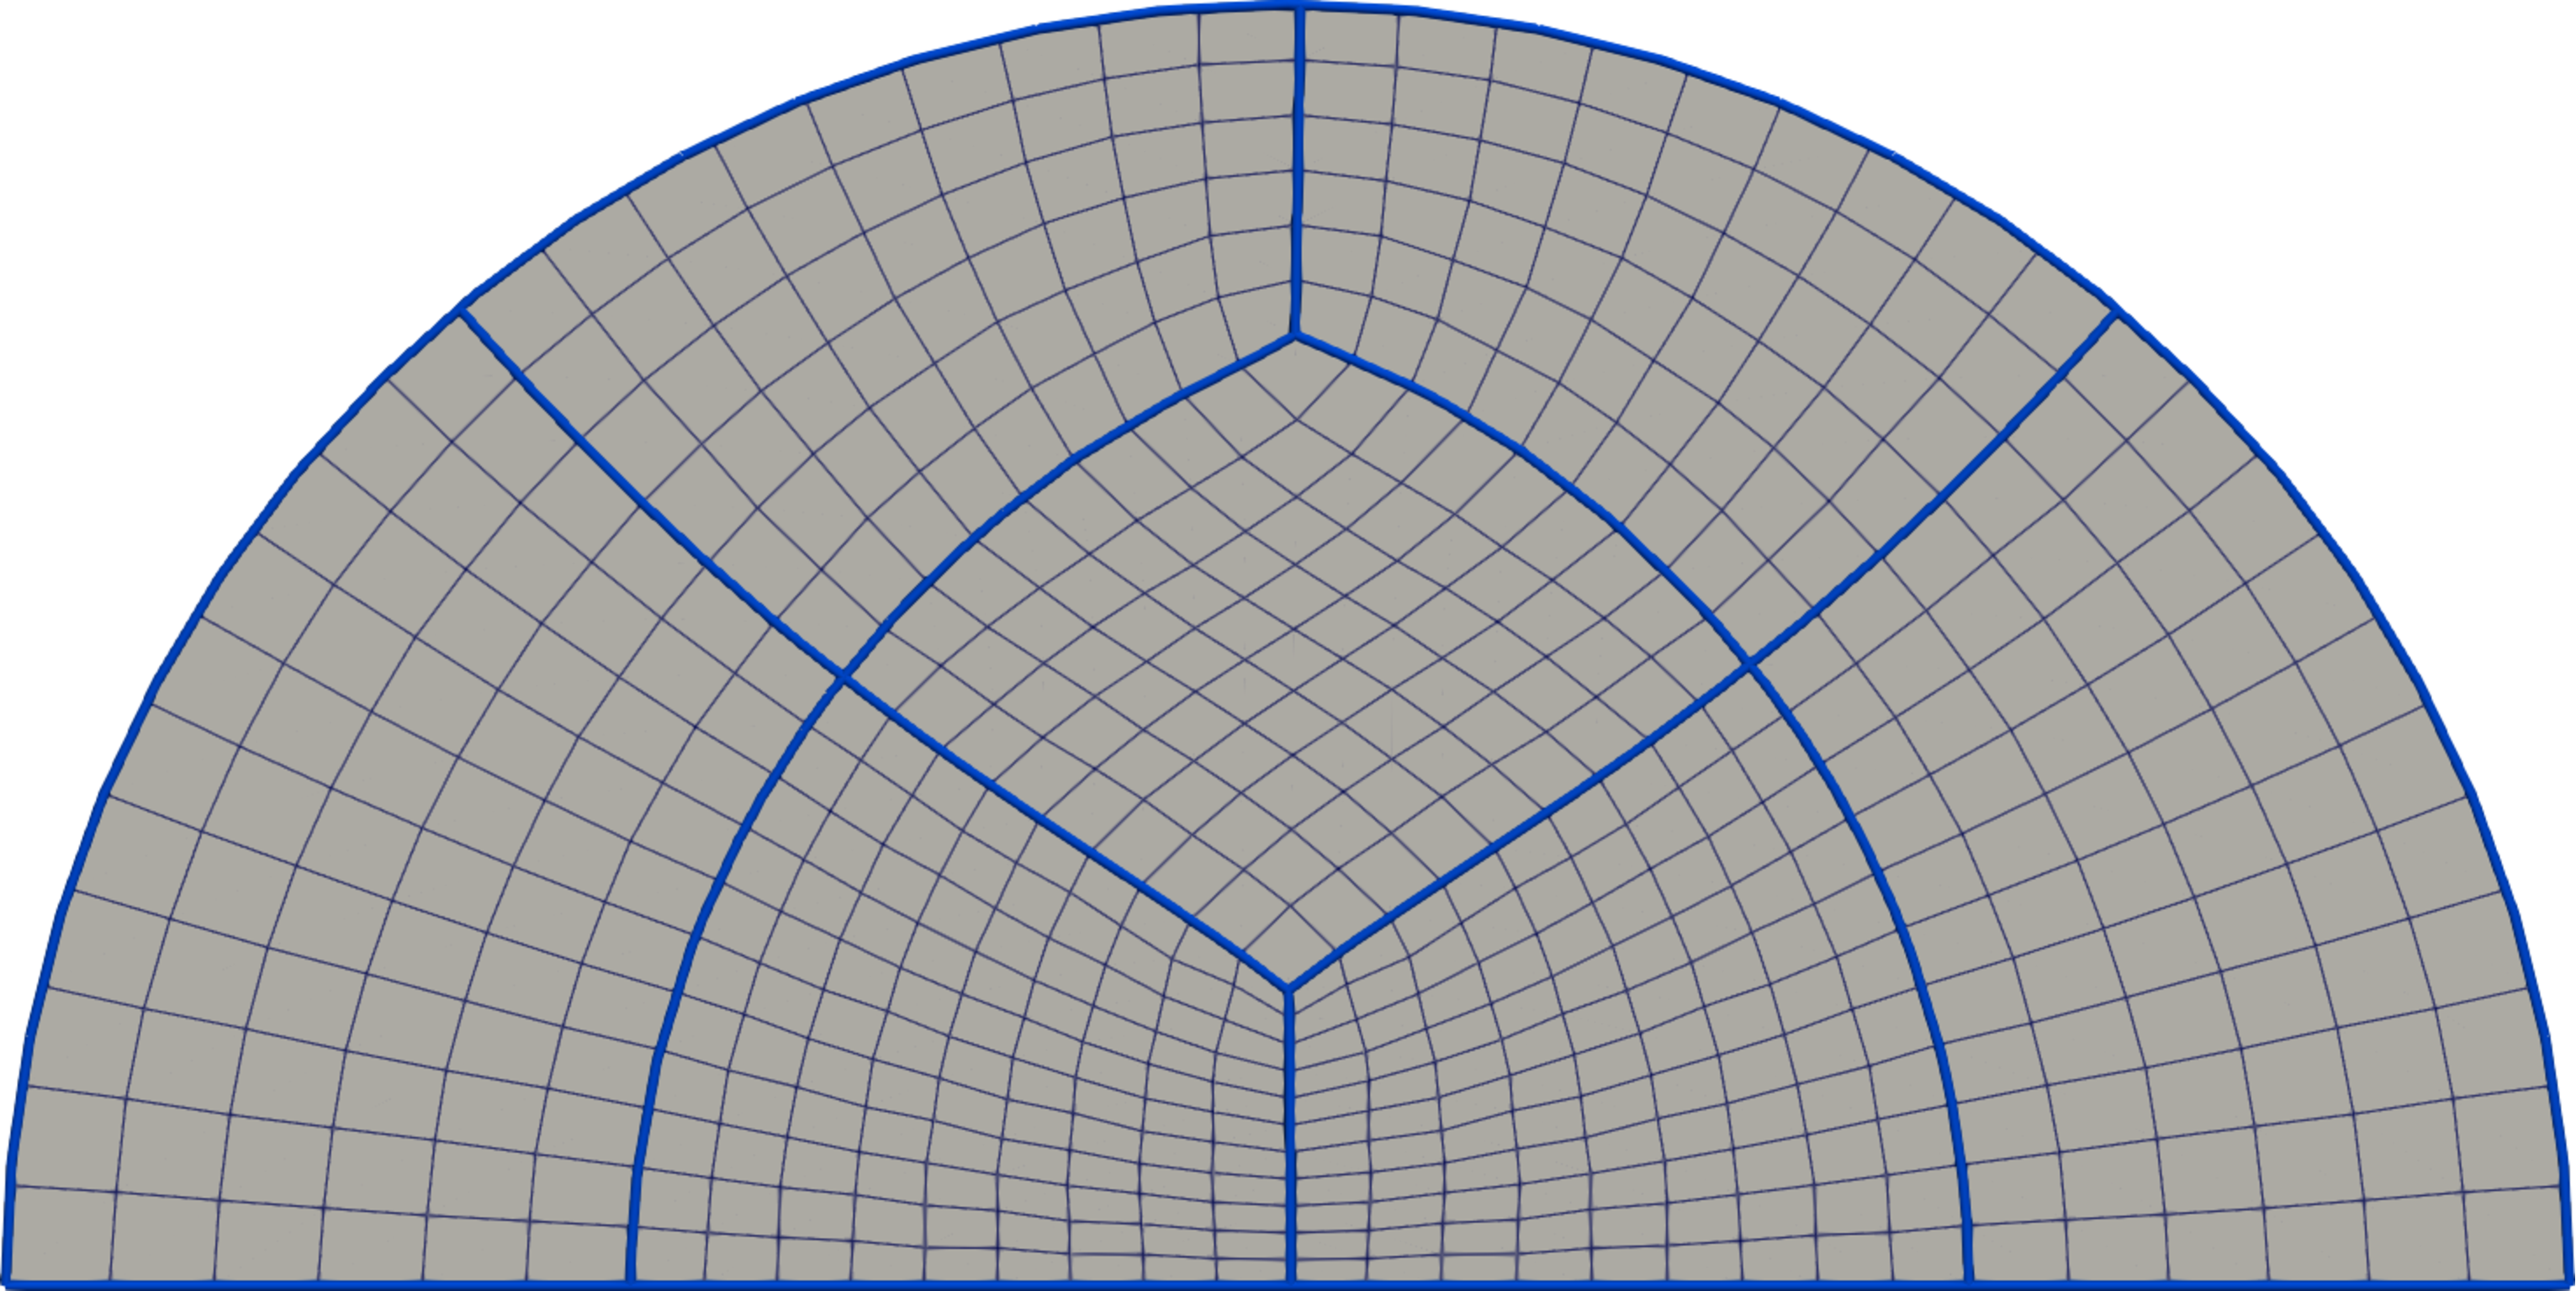
\includegraphics[scale=0.087]{images/demi_disc_align_third.pdf} \hspace{0.2cm}
        \footnotesize Maillage
        \end{column}
    \end{columns}
    \vspace{0.4cm}
        \begin{onerablock}[drop fuzzy shadow]{\small Théorème 1}
    \small
Soit $\Omega$ un domaine borné et fermé dans $\mathbb{R}^2$ avec une frontière régulière par morceau et soit $\bar{u}$ un champ de croix presque-$\mathcal{C}^1$ aligné avec $\partial\Omega$ tel que $0<Card(\mathcal{S}_{\bar{u}})<\infty$ et pour tout $p\in\Omega$, $id_{\bar{u}}(p)=k/4$ où $k\in\mathbb{Z}$ et $k\leq 1$. Si les séparatrices de $\bar{u}$ convergent alors le partitionnement résultant est une décomposition de $\Omega$ en régions à quatre côtés.
    \end{onerablock}
\end{frame}


\begin{frame}{Processus d'alignement}{}

\vspace{-0.3cm}
    \small
    \begin{columns}
    \begin{column}{0.7\textwidth}

\onslide<2->{
\textbf{Idée}: Mise en place d'un processus d'alignement par rotation des croix du bord pour les aligner avec la normale sortante, transformation globale et lisse du champ pour ne pas introduire de singularités.%{\color{onera_gray}( Proposition)}
\\\vspace{0.12cm}
}

\onslide<3->{

\begin{onerablock}[drop fuzzy shadow]{\small Proposition}
    \small
    Soit $\bar{u}$ un champ de croix presque-$\mathcal{C}^1$ sur $\Omega$ et $\theta:\Omega \rightarrow \mathbb{R}$ une fonction de classe $\mathcal{C}^1$ sur $\Omega$, alors $\bar{v}={\mathbf{R}(\theta)\bar{u}}$ est un champ de croix presque-$\mathcal{C}^1$ et pour tout $p\in \Omega\backslash\partial\Omega,~id_{\bar{u}}(p)=id_{\mathbf{R}(\theta)\bar{u}}(p)$.
    \end{onerablock}
    %{\color{onera_gray}(Conservation de certaines propriétés de $\bar{u}$)}\\\vspace{0.12cm}
    {\bf Diffusion de la différence angulaire entre $\bar{u}$ et $\bar{n}$:}
}

\vspace{0.1cm}

\onslide<3->{
%\vspace{0.4cm}
    \begin{equation*}
    \left\{
    \begin{array}{lcll}
    \Delta\phi &=& 0 &\mbox{ dans }\Omega,\\[0.3cm]
    \phi(p) &=& \widehat{(\bar{n}(p); \bar{u}(p))}=\theta_{\bar{n}}(p)-\theta_{\bar{u}}(p)&\mbox{ sur } \partial\Omega.
    \end{array}
    \right.
    \end{equation*}
    {\color{onera_gray}(Angle multivarié, defaut de régularité de $\phi$ et intro. sing. bord, chang. cond. bord.)}\\\vspace{0.12cm}
}


\end{column}

\begin{column}{0.32\textwidth}
        \centering
        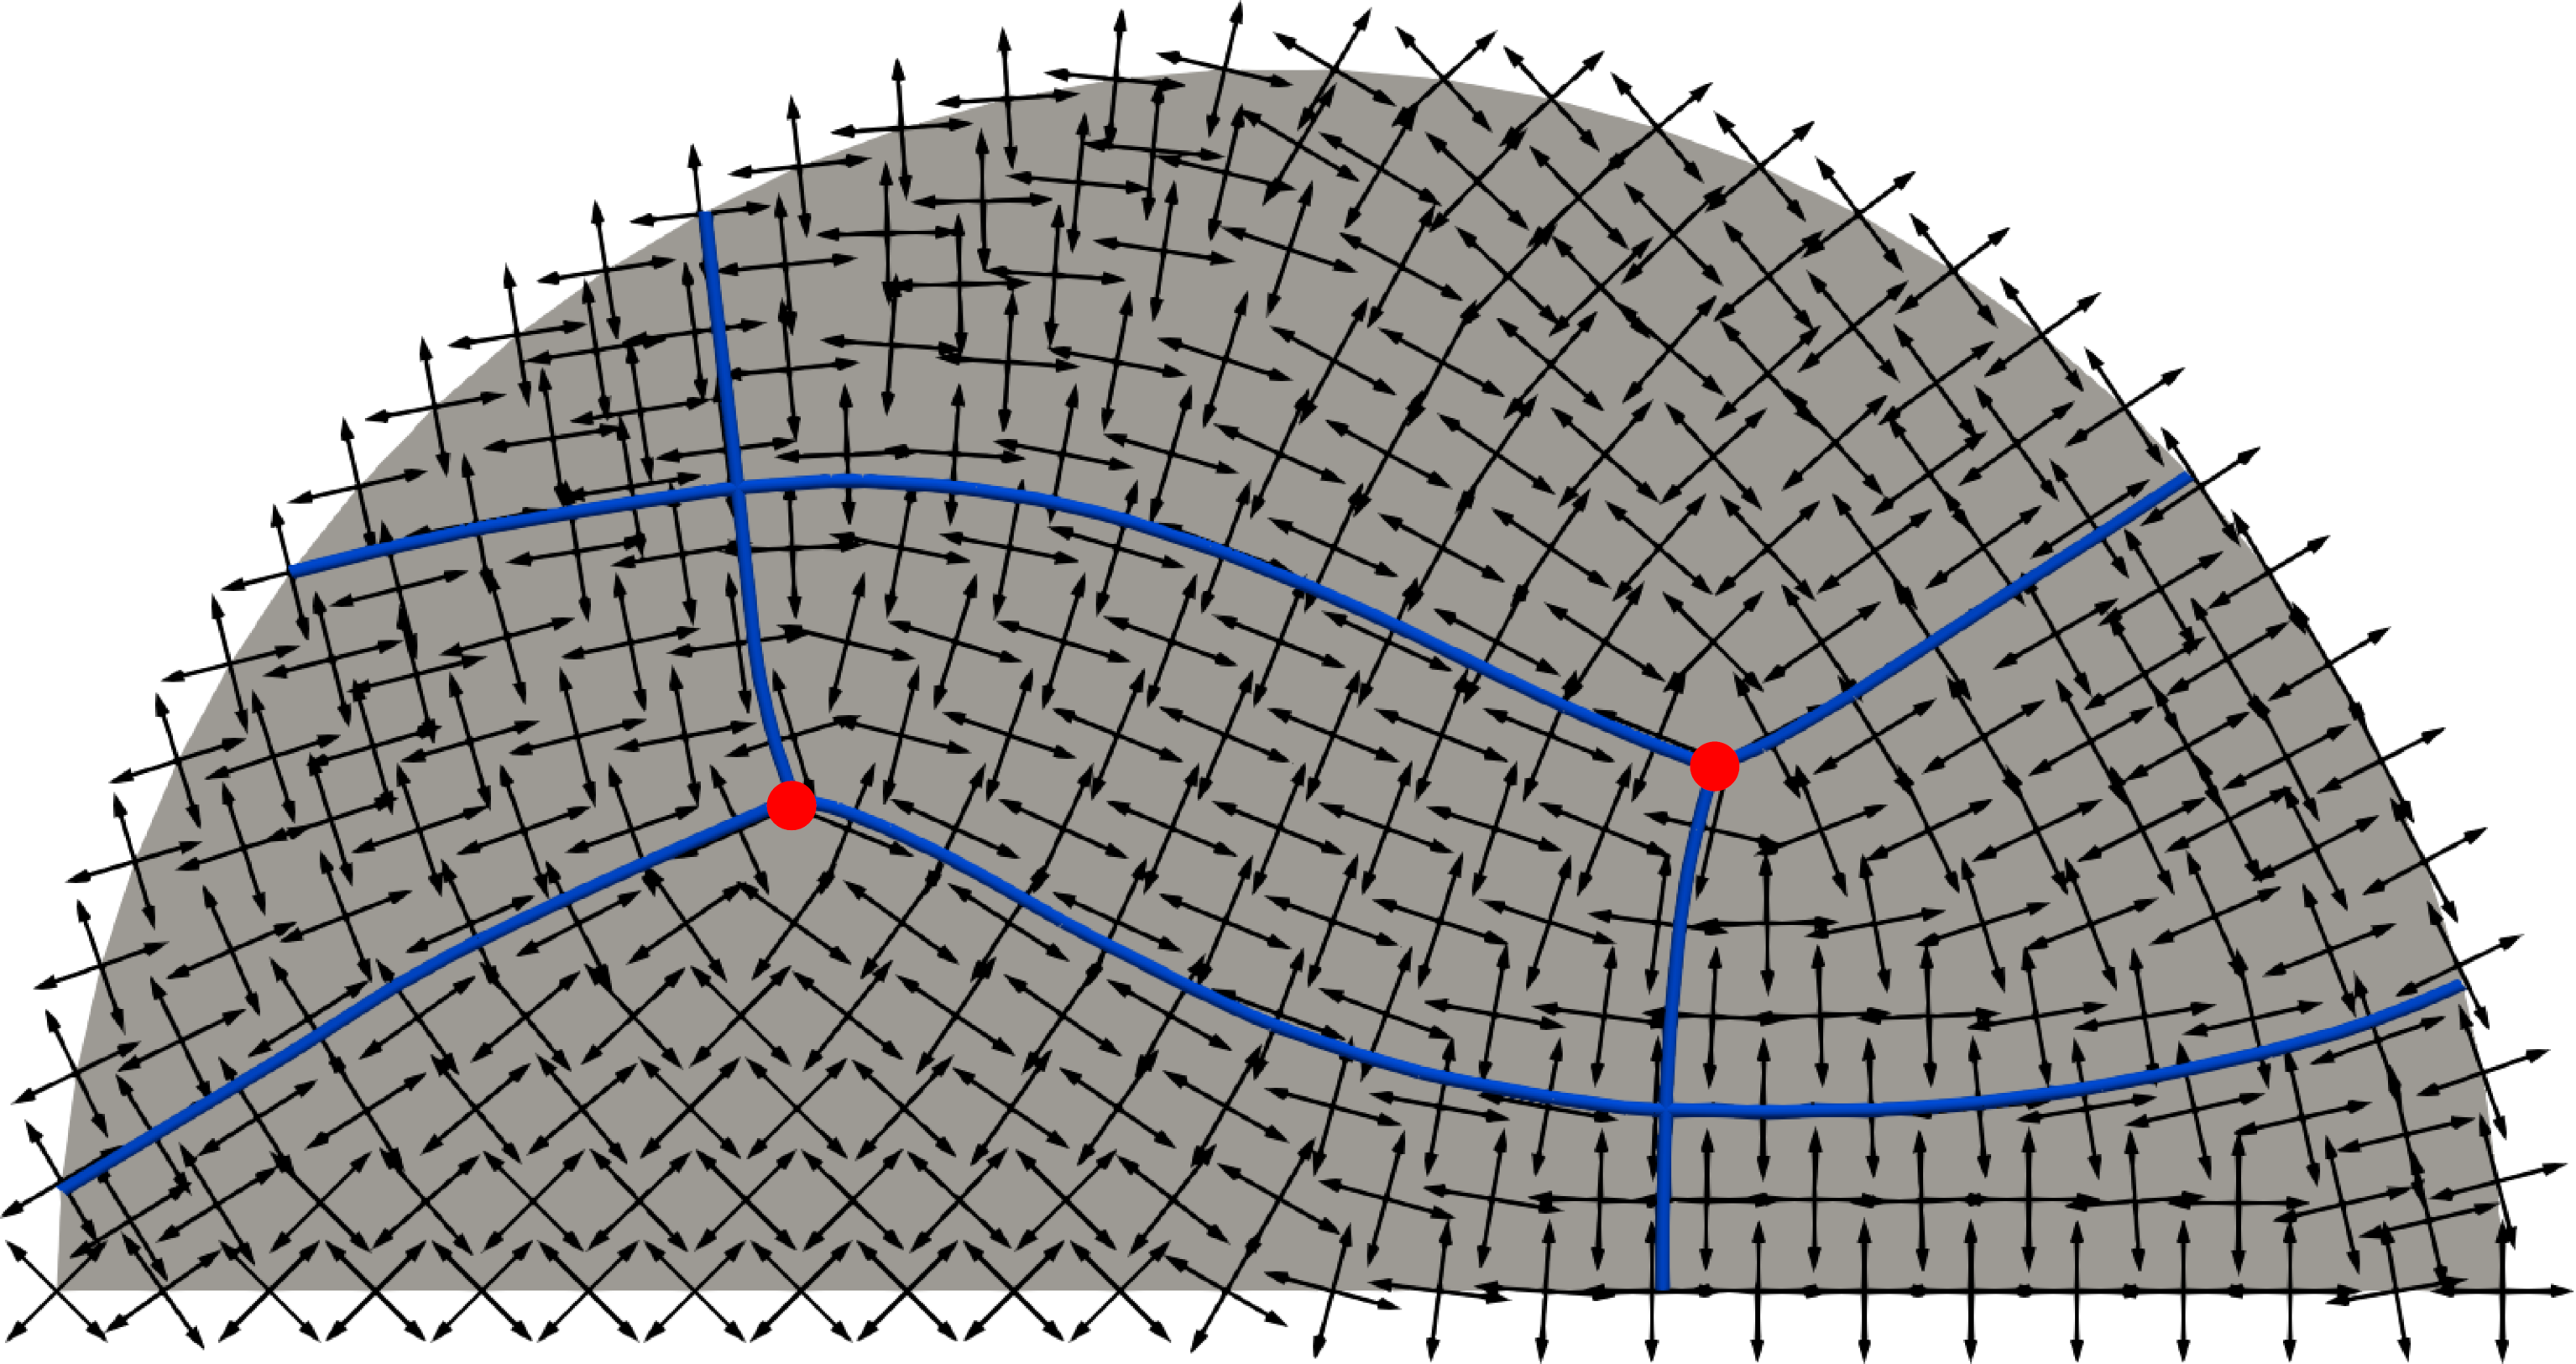
\includegraphics[scale=0.09]{images/mode_prop_stream_non_align_beam.pdf}
        \only<1>{
        \footnotesize {\color{onera_gray}(Le bord ne fait pas partie des séparatrices. Champ de croix non aligné avec le bord du domaine.)}
        }
    \end{column}
    \end{columns}
\end{frame}

\begin{frame}{Processus d'alignement}
\small
\vspace{-0.4cm}
On se donne une paramétrisation \(\gamma\) sur \([0, 1]\) de \(\partial\Omega\).\\\vspace{0.12cm}
\(\theta_{\bar{u}}^\gamma\) et \(\theta_{\bar{n}}^\gamma\) sont des relèvements continus de \(\theta_{\bar{u}}\) et \(\theta_{\bar{n}}\) le long de \(\gamma\).\\\vspace{0.12cm}
\textbf{But} : Lisser l'angle en contrôlant l'emplacement des singularités dues à la non-périodicité des relèvements. L'équation d'alignement devient :\\\vspace{0.12cm}

\begin{equation*}
\left\{
\begin{array}{lcll}
\Delta\phi &=& 0 &\mbox{ dans } \Omega,\\[0.4cm]
\phi(\gamma(t)) &=& \theta_{\bar{n}}^\gamma(t) + \mathcal{I}(t) - \theta_{\bar{u}}^\gamma(t) & \mbox{ sur } \gamma^{-1}(\partial\Omega \backslash (\mathcal{B} \cup \mathcal{S}_{\bar{n}} \cup \mathcal{S}_{\bar{u}})).
\end{array}
\right.
\end{equation*}

\begin{equation*}
\mathcal{I}(t) = \sum_{s \in \gamma^{-1}(\mathcal{B} \cup \mathcal{S}_{\bar{n}})} \left[\underbrace{\left(\pi - \widehat{\gamma(s)}\right)}_{\text{courbure géodésique}} - \underbrace{\left(\lim\limits_{r \rightarrow s^+}\theta^{\gamma}_{\bar{n}}(r) - \lim\limits_{r \rightarrow s^-}\theta^{\gamma}_{\bar{n}}(r)\right)}_{\text{saut de }\bar{n}} - \underbrace{2\pi I_{\gamma(s)}}_{\text{index des pts. de }\mathcal{B}\text{( les coins)}}\right] \mathbb{1}_{[0, t]}(s).
\end{equation*}

On récupère ainsi une régularité \(\mathcal{C}^1\) par morceaux où les sauts sont localisés aux points de l'ens. \(\mathcal{B}\).

\end{frame}


\begin{frame}{Processus d'alignement}
\vspace{-0.2cm}
\small
En généralisant le théorème de Poincarré-Hopf au bord du domaine,
\begin{equation*}
\sum_{s\in Int(\Omega)} id_{\bar{v}}(s)+{\bf \color{red}\sum_{c\in \partial\Omega} id_{\bar{v}}(c)} = \chi(\Omega),
\label{poincareformula_3}
\end{equation*}

on dégage une contrainte générale sur le champ de croix "input":
\begin{equation*}
deg(\bar{u}, \partial\Omega) =\sum_{s\in Int(\Omega)} id_{\bar{u}}(s) = \sum_{s\in Int(\Omega)} id_{\bar{v}}(s) = \chi(\Omega)-\sum_{c\in \partial \Omega} id_{\bar{v}}(c).
\label{third_u_c}
\end{equation*}
\begin{onerablock}[drop fuzzy shadow]{Théorème 2}
Soit $\bar{u}$ un champ de croix tel que pour tout $p\in\Omega\backslash\partial\Omega$, ${\bf id_{\bar{u}}(p)<=1/4}$. \'Etant $\bar{u}$ donné un ensemble $(c_i)_{i\in\{1,\dots,n_b\}}\subset\partial\Omega$ de points distincts tel que:
$
{\bf deg(\bar{u}, \partial\Omega) = \chi(\Omega)-\sum_{i=1}^{n_b} id_{\bar{u}}(c_i),}
$
il existe un champ de croix $\bar{v}$ aligné sur le bord de $\Omega$ et vérifie le Théorème 1.
\end{onerablock}
\vspace{0.1cm}
{\bf Exemple:} Champ de croix construit à partir du mode propre du laplacien sur le demi disque.
\end{frame}


\begin{frame}%{\fontsize{12}{12}\selectfont Exemples}
\vspace{-0.28cm}
\begin{columns}
\begin{column}{0.4\textwidth}
    \centering
    \scriptsize
    $\chi(\Omega)=1$\\\vspace{0.1cm}
    $deg(\bar{u}, \partial\Omega) = 1/4+1/4$\\\vspace{0.1cm}
    $\sum_{i=1}^{2} id_{\bar{u}}(c_i)=1/4+1/4$\\\vspace{0.1cm}
    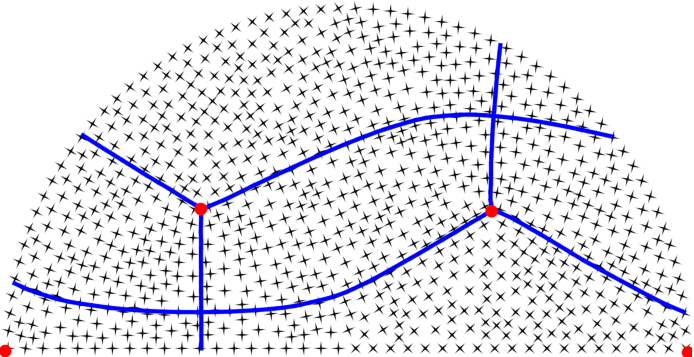
\includegraphics[scale=0.32]{images/demiDiscValPropNonAligne.pdf}\\\vspace{0.1cm}
    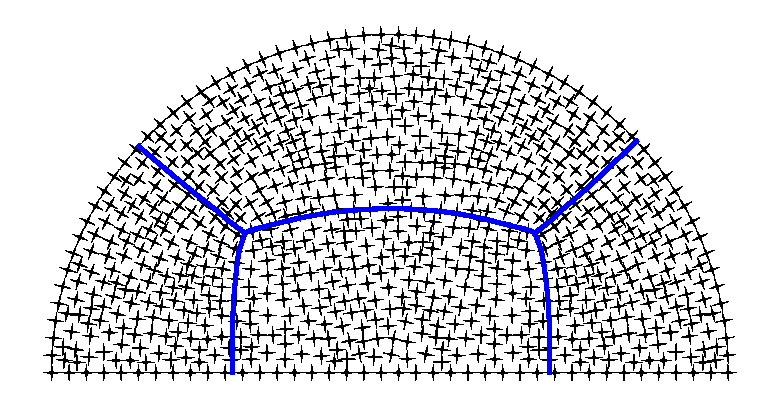
\includegraphics[scale=0.32]{images/demiDiscValPropAligne.eps}\\\vspace{0.1cm}
    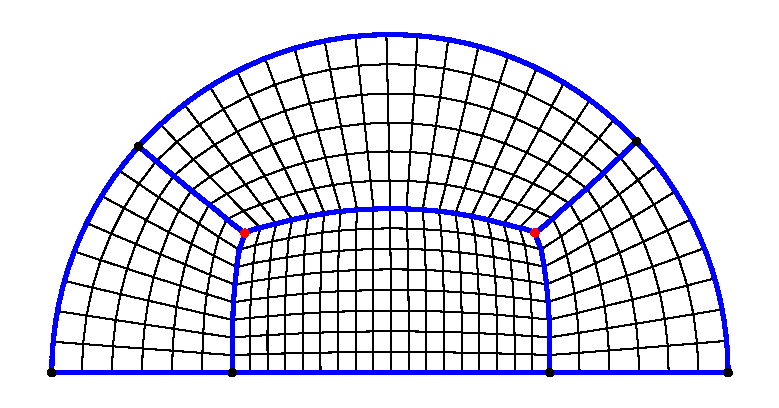
\includegraphics[scale=0.32]{images/mailDemiDisc.eps}\\
    \scriptsize {\color{onera_gray}(Mode propre)}
\end{column}
\pause
\begin{column}{0.4\textwidth}
    \centering
    \scriptsize
    $\chi(\Omega)=1$\\\vspace{0.1cm}
    $deg(\bar{u}, \partial\Omega) = 1/4+1/4$\\\vspace{0.1cm}
    $\sum_{i=1}^{2} id_{\bar{u}}(c_i)=1/4+1/4$\\\vspace{0.1cm}
    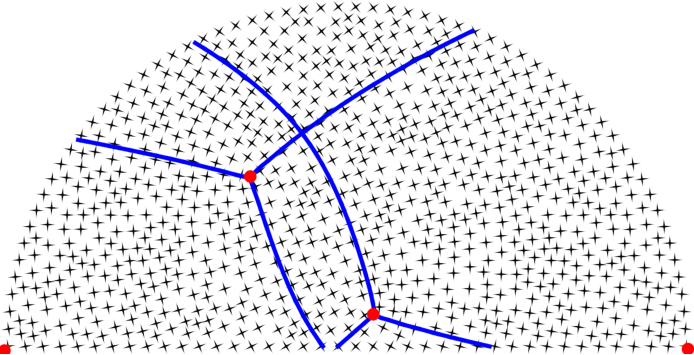
\includegraphics[scale=0.32]{images/demiDiscGinzNonAligne.pdf}\\\vspace{0.1cm}
    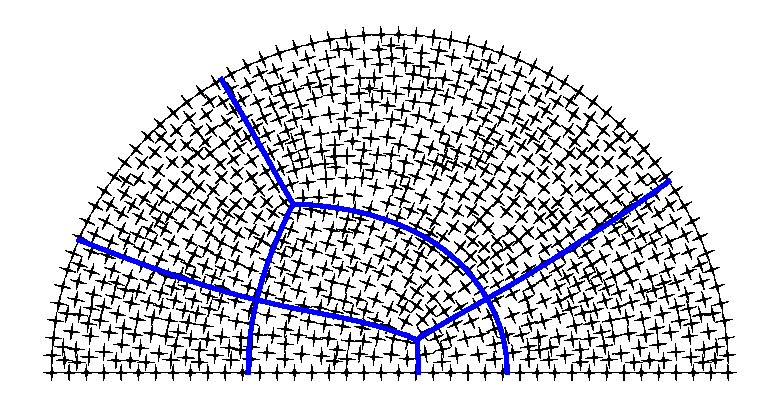
\includegraphics[scale=0.32]{images/demiDiscGinzAligne.eps}\\\vspace{0.1cm}
    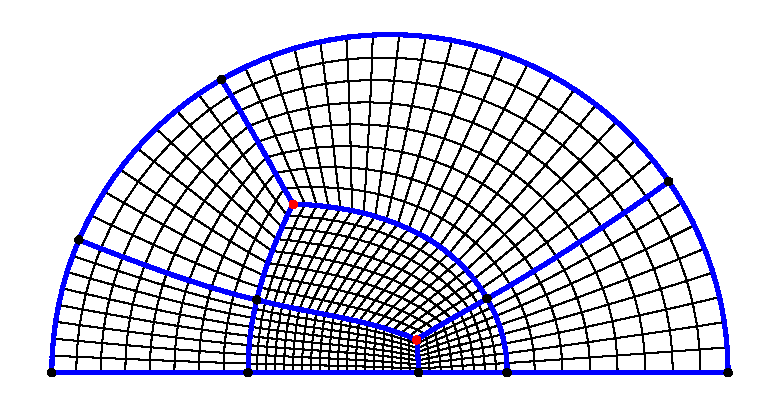
\includegraphics[scale=0.32]{images/demiDiscMail.eps.eps}\\
    \scriptsize {\color{onera_gray}(Champ analytique)}
\end{column}
\pause
\begin{column}{0.4\textwidth}
    \centering
    \scriptsize
    $\chi(\Omega)=1$\\\vspace{0.1cm}
    $deg(\bar{u}, \partial\Omega) = 1/4+1/4+1/4$\\\vspace{0.1cm}
    $\sum_{i=1}^{3} id_{\bar{u}}(c_i)=1/4+1/4-1/4$\\\vspace{0.1cm}
    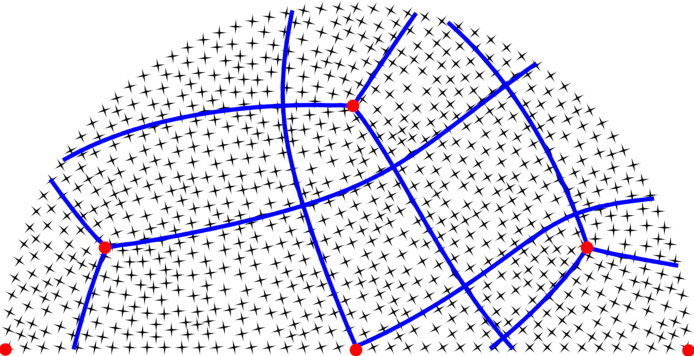
\includegraphics[scale=0.32]{images/demiDiscTroisPointNonAligne.pdf}\\\vspace{0.1cm}
    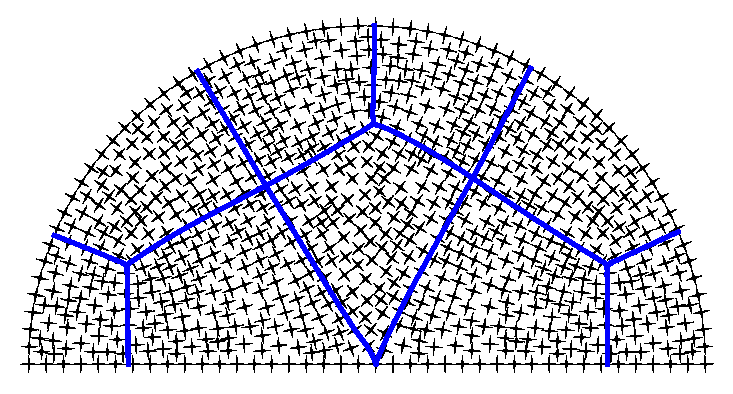
\includegraphics[scale=0.32]{images/demiDIscTroisPointAligne.eps}\\\vspace{0.1cm}
    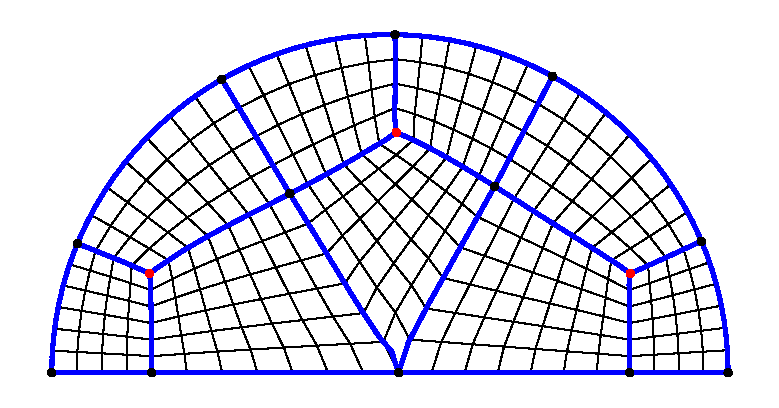
\includegraphics[scale=0.32]{images/mesh_quad_3.eps}\\
    \scriptsize {\color{onera_gray}(bonus pts. sing. bord, vue coin.)}
\end{column}
\end{columns}
\end{frame}


\begin{frame}{Plan}
    %\tableofcontents
    \vspace{-0.4cm}
    \begin{enumerate}
        \item \color{onera} Contexte et objectifs \\\vspace{0.26cm}
        \item Formalisation du processus de partitionnement %{\color{onera_gray}(nouveau point de vue, redressement du champ sur le bord, ...)}
        \vspace{0.26cm}
        \begin{itemize}
            \item Prise en compte de champs de croix arbitraires\\\vspace{0.18cm}
            \item Processus d'alignement\\\vspace{0.18cm}
            \item Domaines non-simplement connexes\\\vspace{0.18cm}
            \item Discussions (quelques résultats théoriques)\\\vspace{0.18cm}
            %\item Exemples%\\\vspace{0.2cm}
        \end{itemize}
        %\item Traitement des singularités de bord {\color{onera_gray}(prise en compte de conditions de bord, ...)}\\\vspace{0.5cm}
        %\item Prise en compte de champs de croix arbitraires {\color{onera_gray}(domaine à trous, multimatériau, ...)}\\\vspace{0.34cm}
        \item Discrétisation et extension aux variétés surfaciques non-planaire %{\color{onera_gray}(prise en compte de la courbure, généralisation, ...)}\\
        \vspace{0.26cm}
        \begin{itemize}
            \item Processus de partitionnement\\\vspace{0.18cm}
            \item Analyse de convergence\\\vspace{0.18cm}
            %\item Exemples%\\\vspace{0.2cm}
        \end{itemize}
        \item Conclusion et perspectives
    \end{enumerate}
\end{frame}



\begin{frame}{Domaines non-simplement connexes}
\small
\vspace{-0.5cm}
\begin{columns}
\begin{column}{0.85\textwidth}
%\vspace{0.08cm}
{\color{onera_gray}(Domaine d'un seul tenant avec plusieurs bords, qui ne peuvent être continuellement réduit à un point, domaines à trous)}\\\vspace{0.08cm}
%\textbf{Application sur un domaine à trou:}
Soit $\partial\Omega=\cup_i\Gamma_i$, avec $(b_j^i)_{i,j}$ les points singuliers de bord.\\\vspace{0.12cm}
%\vspace{0.08cm}
La contrainte sur $\bar{u}$ devient:
    $deg(\bar{u}, \partial\Omega)=\sum_i deg(\bar{u},\Gamma_i)=\chi(\Omega)-\sum_i\sum_jid_{\bar{u}}(b_j^i).$\\\vspace{0.12cm}
%\vspace{-0.1cm}
%\\[-0.1cm]
\textbf{Exemple:} Carré troué, $\chi(\Omega)=0, \sum_i\sum_jid_{\bar{u}}(b_j^i)=-1/4-1/4-1/4-1/4$\\\vspace{0.12cm}
On peut prendre $\bar{u}$ tel que $deg(\bar{u}, \partial\Omega)=-1/4-1/4-1/4-1/4$\\\vspace{0.12cm}
{\color{onera_gray} Echec du processus d'alignement. Non régularité du champ dû à la non-périodicité de la différence des croix sur les bords (voir figure).}\\\vspace{0.08cm}
\end{column}
\begin{column}{0.18\textwidth}
\centering
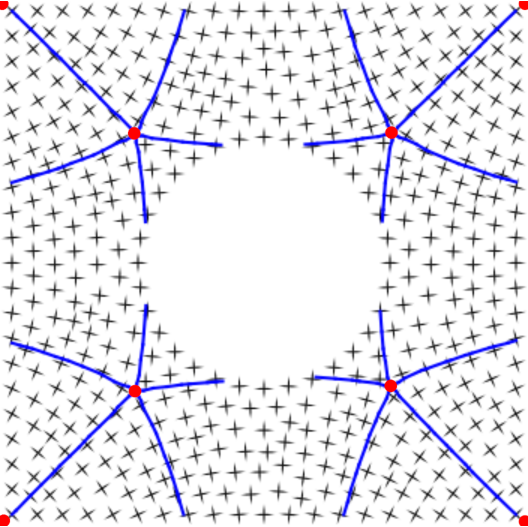
\includegraphics[scale=0.32]{images/carreDiscVide_stream_non_align_beam.pdf}
\end{column}
\end{columns}
\vspace{0.05cm}
\centering
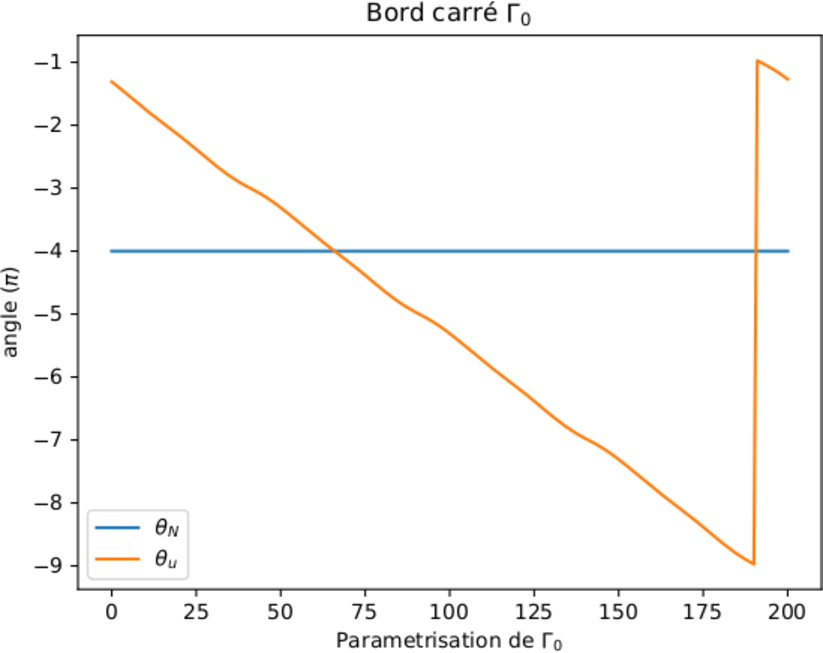
\includegraphics[width=6cm, height=2.45cm]{images/courbe_1.pdf}\hspace{0.6cm}
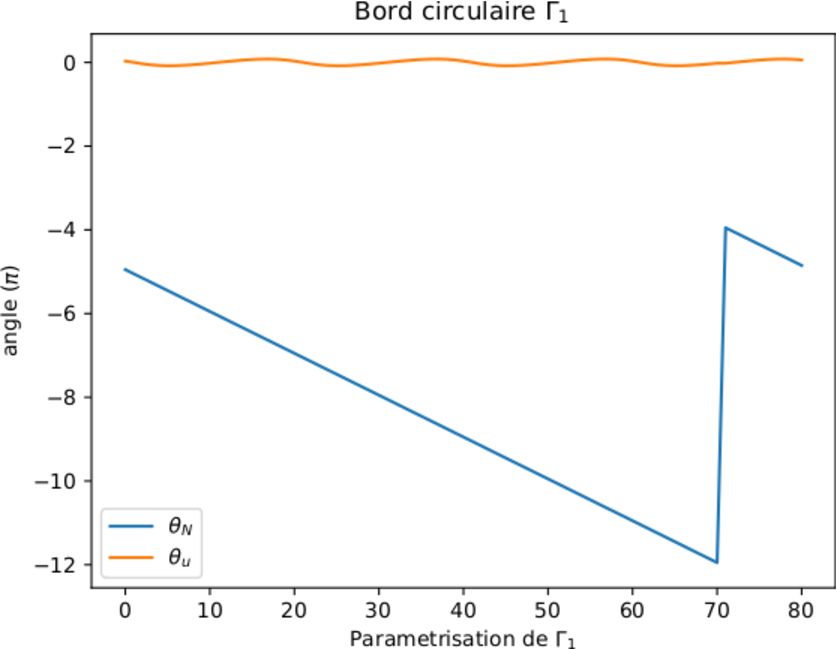
\includegraphics[width=6cm, height=2.45cm]{images/courbe_0.pdf}
\end{frame}



\begin{frame}{Domaines non-simplement connexes}{}
\small
Pour que ça marche, il faut que le champ de croix $\bar{u}$ vérifie:\\\vspace{0.2cm}
\begin{equation*}
\left\{
\begin{array}{lcll}
   deg(\bar{u},\Gamma_0)&=&2\pi-2\pi\sum_j id_{\bar{u}}(b_j^0)&\mbox{ sur }\Gamma_0,\\[0.3cm]
   deg(\bar{u}, \Gamma_i)&=&-2\pi-2\pi\sum_j id_{\bar{u}}(b_j^i)&\mbox{ sur }\Gamma_i~~~\forall~i.
\end{array}
\right.
\end{equation*}
\\\vspace{0.2cm}
{\color{onera_gray} Il s'agit de la même condition que précédemment mais imposée sur chaque bord.}\\\vspace{0.12cm}
Nous récupérons cette condition grâce au champ de correction vérifiant l'équation faible suivante :
\vspace{0.12cm}
\begin{equation*}
\left\{
\begin{array}{lcll}
    \triangle h &= &0 &\mbox{ dans }\Omega,\\[0.25cm]
    \displaystyle\frac{1}{2\pi}\int_{\Gamma_0}\theta_h &=& deg(\bar{u}, \Gamma_0)-1+\sum_j id_{\bar{u}}(b_j^0))&\mbox{ sur } \Gamma_0,\\[0.25cm]
    \displaystyle\frac{1}{2\pi}\int_{\Gamma_i}\theta_h& =& deg(\bar{u}, \Gamma_i)-1-\sum_j id_{\bar{u}}(b_j^i),&\mbox{ sur }\Gamma_i~~~\forall~i.
\end{array}
\right.
\end{equation*}

\end{frame}

\begin{frame}{Domaines non-simplement connexes}

\vspace{-0.3cm}
\small
\begin{columns}
\begin{column}{0.68\textwidth}
L'équation d'alignement prend alors la forme suivante : {\color{onera_gray} (où on a pris en compte le champ de correction dans la condition de bord.)}
%{\color{onera}
\begin{equation*}
\left\{
\begin{array}{lcll}
    \triangle\phi& =& 0& \mbox{ dans }\Omega,\\[0.25cm]
    \phi &=& \theta_{\bar{n}_{|\Gamma_i}}-\theta_{\bar{u}_{|\Gamma_i}}-\theta_{h_{|\Gamma_i}}& \mbox{ sur }\Gamma_i, \forall i.
\end{array}
\right.
\end{equation*}
%}{\color{red}\rightarrow v=R(\phi)R(\theta_h/4)u}\\
%}
Champ de croix finale {\color{onera_gray} (obtenue via une double rotation, champ cor., champ align.)}
\begin{equation*}
\bar{v}=R(\phi)R(\theta_h)\bar{u}.
\end{equation*}
\textbf{Exemple:} Application au carré troué.\\\vspace{0.2cm}
\begin{onerablock}[drop fuzzy shadow]{
\small Théorème 3}
\'Etant $\bar{u}$ donné un ensemble $(c_i)_{i\in\{1,\dots,n_b\}}\subset\partial\Omega$ de points distincts tel que:
$
{\bf deg(\bar{u}, \partial\Omega) = \chi(\Omega)-\sum_{i=1}^{n_b} id_{\bar{u}}(c_i),}
$
le champ de croix $\bar{v}=R(\phi)R(\theta_h)\bar{u}$ vérifie le Théorème 1.
\end{onerablock}
\end{column}
\begin{column}{0.32\textwidth}
\centering
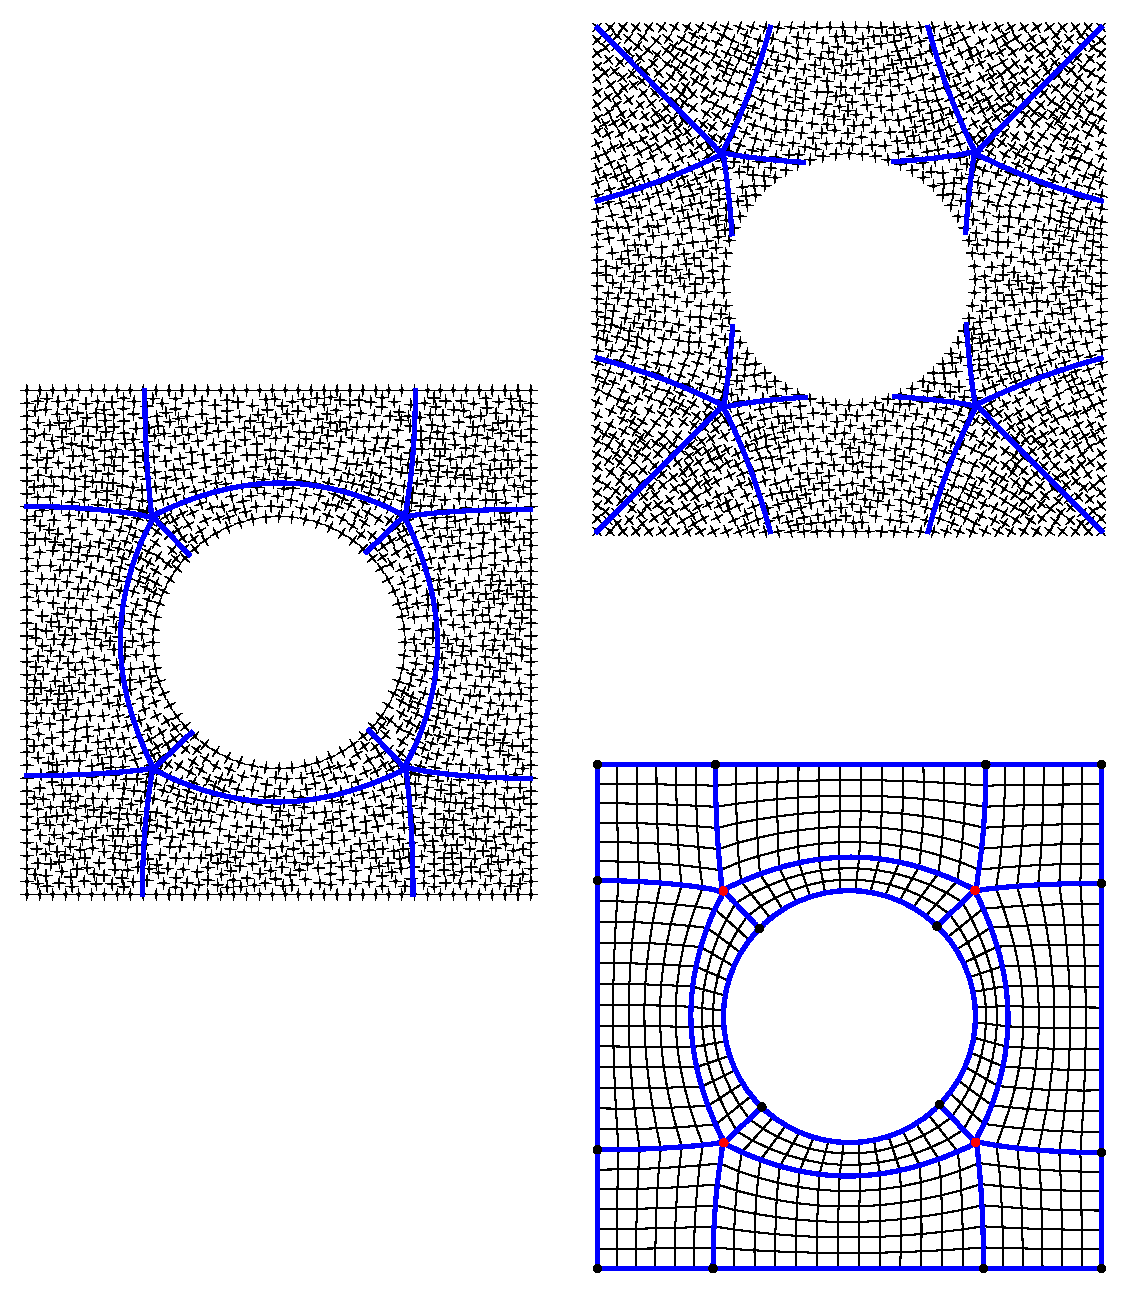
\includegraphics[scale=0.27]{images/image.eps}
\end{column}
\end{columns}
\end{frame}

\begin{frame}{Exemples}%{ Quelques domaines à trous et un domaine avec plusieurs composants connexes}
\vspace{-0.25cm}
\begin{columns}
\begin{column}{0.34\textwidth}
    \centering
    \onslide<1->{\includegraphics[scale=0.35]{images/1_beam.png}\\\vspace{0.1cm}
    \scriptsize
    $\chi(\Omega)=0$; $deg(\bar{u}, \partial\Omega) = -1/4-1/4$\\\vspace{0.1cm}
    $\sum_{i=1}^{5} id_{\bar{u}}(c_i)=1/4+1/4+1/4+1/4-1/2$\\\vspace{0.1cm}\vspace{0.6cm}
    \includegraphics[scale=0.35]{images/2.png}}
\end{column}
\begin{column}{0.34\textwidth}
    \centering
    \onslide<2->{\includegraphics[scale=0.35]{images/3_beam.png}\\\vspace{0.1cm}
    \scriptsize
    $\chi(\Omega)=0$; $deg(\bar{u}, \partial\Omega) = -1/4-1/4$\\\vspace{0.1cm}
    $\sum_{i=1}^{5} id_{\bar{u}}(c_i)=1/4+1/4+1/4+1/4-1/2$\\\vspace{0.1cm}\vspace{0.6cm}
    \includegraphics[scale=0.35]{images/4.png}}
\end{column}
\begin{column}{0.34\textwidth}
    \centering
    %\includegraphics[scale=0.31]{images/mesh_quad_6.pdf}\\\vspace{-0.2cm}
    %\scriptsize\color{onera_gray}{ Multi-materiau }
    \onslide<3->{\includegraphics[scale=0.35]{images/mailNautilus.eps}\\\vspace{0.1cm}
    \scriptsize
    $\chi(\Omega)=0$\\\vspace{0.1cm}
    $deg(\bar{u}, \partial\Omega) = 1/4+1/4+1/4+1/4-1/4-1/4-1/4-1/4$\\\vspace{0.1cm}
    $\sum_{i=1}^{2} id_{\bar{u}}(c_i)=1/4-1/4$\\\vspace{0.2cm}
    %\includegraphics[scale=0.35]{images/mailNautilus.eps}\\\vspace{-0.1cm}
    \scriptsize\color{onera_gray}{ Nautilus}}
\end{column}
\end{columns}
\end{frame}


\begin{frame}{Plan}
    %\tableofcontents
    \vspace{-0.4cm}
    \begin{enumerate}
        \item \color{onera} Contexte et objectifs \\\vspace{0.26cm}
        \item Formalisation du processus de partitionnement %{\color{onera_gray}(nouveau point de vue, redressement du champ sur le bord, ...)}
        \vspace{0.26cm}
        \begin{itemize}
            \item Prise en compte de champs de croix arbitraires\\\vspace{0.18cm}
            \item Processus d'alignement\\\vspace{0.18cm}
            \item Domaines non-simplement connexes\\\vspace{0.18cm}
            \item Discussions (quelques résultats théoriques)\\\vspace{0.18cm}
            %\item Exemples%\\\vspace{0.2cm}
        \end{itemize}
        %\item Traitement des singularités de bord {\color{onera_gray}(prise en compte de conditions de bord, ...)}\\\vspace{0.5cm}
        %\item Prise en compte de champs de croix arbitraires {\color{onera_gray}(domaine à trous, multimatériau, ...)}\\\vspace{0.34cm}
        \item Discrétisation et extension aux variétés surfaciques non-planaire %{\color{onera_gray}(prise en compte de la courbure, généralisation, ...)}\\
        \vspace{0.26cm}
        \begin{itemize}
            \item Processus de partitionnement\\\vspace{0.18cm}
            \item Analyse de convergence\\\vspace{0.18cm}
            %\item Exemples%\\\vspace{0.2cm}
        \end{itemize}
        \item Conclusion et perspectives
    \end{enumerate}
\end{frame}


\begin{frame}{Discussions}{Sur l'initialisation des séparatrices}

\vspace{-0.3cm}
\small
\only<1>{
\begin{columns}
\begin{column}{0.7\textwidth}

L'initialisation des séparatrices pose un problème bien connu dans les EDOs qui est de savoir \textbf{comment tracer une ligne de champ à partir d'un point singulier donné ?}\\\vspace{0.15cm}
Nous proposons le résultat suivant:\\\vspace{0.15cm}
\begin{onerablock}[drop fuzzy shadow]{\small Proposition 1}
Soit $\bar{u}$ un champ de croix presque-$\mathcal{C}^1$ et $p\in \Omega\backslash\partial\Omega$. Soit $V_p\subset\Omega$ un voisinnage de $p$ tel que le bord $\partial V_p$ de $V_p$ est de classe $\mathcal{C}^1$ et $\partial V_p\cap\mathcal{S}_{\bar{u}}=\emptyset$. On suppose de plus que $V_p$ est étoilé par rapport à $p$. Alors il existe un champ de croix $\bar{v}$ tel que:\\[-0.3cm]
\begin{enumerate}
\item $\bar{v}$ est presque-$\mathcal{C}^1$ sur $\Omega$,\\[-0.3cm]
\item $\mathcal{S}_{\bar{v}}\cap V_p =\{p\}$ et $id_{\bar{v}}(p)=\sum_{q\in \mathcal{S}_{\bar{u}}\cap V_p} id_{\bar{u}}(q)$,\\[-0.3cm]
\item pour tout $q\in \partial V_p$ tel que $\overrightarrow{v_q}:=\overrightarrow{pq}.\|\overrightarrow{pq}\|^{-1}\in \bar{u}(q)$, le point $p$ appartient à la ligne de champ $SL_{\bar{v}}(q,\overrightarrow{v_q})$.\\[-0.3cm]
\end{enumerate}
\end{onerablock}

\end{column}
\begin{column}{0.3\textwidth}
\centering
\includegraphics[scale=0.2]{images/illustr_etoilage.pdf}
Construction du champ
\end{column}
\end{columns}
\
}

\only<2>{
Ce qui permet d'avoir le résultat suivant donnat le nombre de séparatrices ainsi que leur direction de sortie (à $\pi/2$ les uns des autres)
\vspace{0.25cm}
\begin{onerablock}[drop fuzzy shadow]{\small Proposition 2}
\small
Soit $p\in\Omega\backslash\partial\Omega$ tel que $id_{\bar{u}}(p)=k/4$ avec $k\in\mathbb{Z}$ et $k\leq 1$. Il existe une suite de points $(t_i)_{i\in\llbracket1, N_s\rrbracket}$ tel que $N_s=4-k$ et $0\leq t_1\leq\dots\leq t_{N_s}\leq 1$ avec $\overrightarrow{p\gamma(t_i)}.\|\overrightarrow{p\gamma(t_i)}\|^{-1}\in\bar{u}(\gamma(t_i))$. De plus pour tout $i\in\llbracket 1, N_s\rrbracket$, $\int_{t_i}^{t_{i+1}}dW_p^\gamma=-\frac{\pi}{2},\mbox{ où }t_{N_s+1}:=t_1.$
\end{onerablock}

\vspace{0.25cm}
Version de bord:
\vspace{0.25cm}

\begin{onerablock}[drop fuzzy shadow]{\small Proposition 3}
\small
Soit $p\in\partial\Omega$ tel que $id_u(p)=k/4$ avec $k\in\mathbb{Z}$ et $k\leq 1$. Au point $p$, il y a $N_s=3-k$ séparatrices qui convergent, incluant les frontières de $\Omega$, divisant ainsi le voisinage de $p$ en $2-k$ secteurs. De plus, à l'intérieur de chaque secteur, on a: $\int_0^1W_p^\gamma(t)dt=-\frac{\pi}{2}.$
\end{onerablock}

}

\end{frame}


\begin{frame}{Discussions}{Sur la signification pratique de l'hypothèse $0<Card(\mathcal{S}_{\bar{u}})<\infty$}
\centering
    \small
\begin{onerablock}[drop fuzzy shadow]{\small Théorème 1}
    \small
Soit $\Omega$ un domaine borné et fermé dans $\mathbb{R}^2$ avec une frontière régulière par morceau et soit $\bar{u}$ un champ de croix presque-$\mathcal{C}^1$ aligné avec $\partial\Omega$ tel que $0<Card(\mathcal{S}_{\bar{u}})<\infty$ et pour tout $p\in\Omega$, $id_{\bar{u}}(p)=k/4$ où $k\in\mathbb{Z}$ et $k\leq 1$. Si les séparatrices de $\bar{u}$ convergent alors le partitionnement résultant est une décomposition de $\Omega$ en régions à quatre côtés.
\end{onerablock}
{\bf\footnotesize\color{onera_gray} Le champ radial sur l'anneau est aligné avec le bord. Mais on a pas de partitions à 4 côtés.}\\
\begin{columns}
\begin{column}{0.33\textwidth}
\centering
    \onslide<1->{
\includegraphics[scale=0.11]{images/anneau_with_cross.pdf}
}
\end{column}

\begin{column}{0.33\textwidth}
\centering
    \onslide<2->{
\includegraphics[scale=0.12]{images/anneau_cross.pdf}
}
\end{column}

\begin{column}{0.33\textwidth}
\centering
    \onslide<2->{
\includegraphics[scale=0.36]{images/anneau_mail.pdf}
}
\end{column}
\end{columns}
\vspace{0.3cm}
\end{frame}


\begin{frame}{Discussions}{Sur les multi-matériaux}
\centering
\includegraphics[scale=0.38]{images/carreDiscPleinCouper domain.pdf}\hspace{0.5cm}
\includegraphics[scale=0.57]{images/mesh_quad_6.pdf}
\end{frame}


\begin{frame}{Overview}
    %\tableofcontents
    \vspace{-0.4cm}
    \begin{enumerate}
        \item \color{onera} Contexte et objectifs \\\vspace{0.34cm}
        \item Formalisation du processus de partitionnement %{\color{onera_gray}(nouveau point de vue, redressement du champ sur le bord, ...)}
        \vspace{0.32cm}
        \begin{itemize}
            \item Prise en compte de champs de croix arbitraires\\\vspace{0.2cm}
            \item Processus d'alignement\\\vspace{0.2cm}
            \item Domaines non-simplement connexes\\\vspace{0.2cm}
            %\item Exemples%\\\vspace{0.2cm}
        \end{itemize}
        %\item Traitement des singularités de bord {\color{onera_gray}(prise en compte de conditions de bord, ...)}\\\vspace{0.5cm}
        %\item Prise en compte de champs de croix arbitraires {\color{onera_gray}(domaine à trous, multimatériau, ...)}\\\vspace{0.34cm}
        \item Discrétisation et extension aux variétés surfaciques non-planaire %{\color{onera_gray}(prise en compte de la courbure, généralisation, ...)}\\
        \vspace{0.32cm}
        \begin{itemize}
            \item Processus de partitionnement\\\vspace{0.2cm}
            \item Analyse de convergence\\\vspace{0.2cm}
            %\item Exemples%\\\vspace{0.2cm}
        \end{itemize}
        \item Conclusion et perspectives
    \end{enumerate}
\end{frame}



\begin{frame}{Processus de partitionnement}{Représentation du champ de croix}
%\vspace{-0.16cm}
\small
\begin{columns}
    \begin{column}{0.8\textwidth}
\onslide<1->{
Soit $\Omega_h$ un maillage triangulaire d'un domaine $\Omega$ et  $\bar{u}$ un champ de croix donné sur $\Omega$. On cherche à définir $\bar{u}_h$\\\vspace{0.15cm}
$\delta\theta(\bar{u}(s_i),\bar{u}(s_j))$ écart angulaire entre $\bar{u}(s_i)$ et $\bar{u}(s_j)$ {\color{onera_gray} (différence angulaire entre deux croix aux sommets d'une même arête).}\vspace{0.15cm}
        }
\onslide<2->{
\begin{onerablock}[drop fuzzy shadow]{\small Définition}
\small
Un triangle $T$ de sommets $s_1$, $s_2$ et $s_3$ est dit singulier si:%'il vérifie l'une des propriétés suivantes:
 \begin{itemize}
  \item il existe $i\in\llbracket 1, 3\rrbracket$ tel que $\bar{u}(s_i)=0$ \textbf{ou},\\%[-0.2cm]
  \item il existe  $i,j\in\llbracket 1, 3\rrbracket$, tel que  $\delta\theta(\bar{u}(s_i),\bar{u}(s_j))$ n'est pas défini \textbf{ou},\\%[-0.2cm]
  \item pour tout $i\in\llbracket 1, 3\rrbracket$, $\bar{u}(s_i)\neq 0$ et $\sum_{i=1}^3\delta\theta(\bar{u}(s_i),\bar{u}(s_{i+1}))\neq 0$ {\color{onera_gray} (revient au calcul de l'index d'un point quelconque dans le triangle).}
 \end{itemize}
\end{onerablock}
}
\onslide<3->{
Les zones singulières sont des agrégas de triangles singuliers.
\\\vspace{0.15cm}
\textbf{Exemples:} (voir figure)
\\\vspace{0.4cm}
}

    \end{column}

    \begin{column}{0.2\textwidth}
    \centering
\only<1>{
\vspace{-0.1cm}
    \includegraphics[scale=0.14]{images/illustr_delta.pdf}  \\\vspace{0.8cm}}
\only<2>{
    \includegraphics[scale=0.11]{images/illustr_delta.pdf}  \\\vspace{0.2cm}
    \includegraphics[scale=0.11]{images/zone_singuliere_1.pdf}  \\\vspace{0.2cm}}
\only<3>{
    \includegraphics[scale=0.11]{images/zone_singuliere_1.pdf}  \\\vspace{0.2cm}
    \includegraphics[scale=0.11]{images/zone_singuliere_2.pdf} \vspace{0.2cm}}
    %\footnotesize Partitionnement
    \end{column}
\end{columns}
\end{frame}

\begin{frame}{Processus de partitionnement}{Représentation du champ de croix}
\begin{columns}
    \begin{column}{0.72\textwidth}
    \vspace{-0.1cm}
        \small
Le champ de croix $\bar{u}_h(p)$ est défini sur $\Omega_h$ par:
\begin{itemize}
\item[$\bullet$] si $p$ est un sommet de $\Omega_h$ n'appartenant pas a une zone singulière, alors $\bar{u}_h(p)=\bar{u}(p)$.\\%[-0.3cm]
\item[$\bullet$] si $p$ n'appartient pas à une zone singulière alors il appartient à un triangle non singulier.
$$
\left\{
\begin{array}{l}
\bar{u}_h(p)=\displaystyle\left\{\mathbf{R}\left(\theta_p+m\frac{\pi}{2}\right)(1,0)^t,~m\in\mathbb{Z}\right\},\\[0.2cm]
\theta_p=\sum_{i\in\llbracket1, 3\rrbracket}\lambda_i\theta_i.
\end{array}
\right.
$$
\item[$\bullet$] si $p$ appartient à une zone singulière alors:
\begin{equation*}
\label{eqn:etoilage}
\left\{
\begin{array}{l}
\bar{u}_h(p)=\bar{u}_h(\widetilde{p}),\\[0.2cm]
\{\widetilde{p}\}=[S_Zp)\cap\partial Z.
\end{array}
\right.
\end{equation*}
\end{itemize}
\vspace{-0.15cm}
\textbf{Conséquences:} (voir figure)
\vspace{0.2cm}
\end{column}

\begin{column}{0.2\textwidth}
\centering
\includegraphics[scale=0.09]{images/u_sing.pdf}
\scriptsize Un point d'index 1
%\\\vspace{0.2cm}
\includegraphics[scale=0.09]{images/u_h_sing.pdf}
\scriptsize 6 d'index 1/4 et 2 d'index -1/4 \vspace{0.2cm}
\end{column}
\end{columns}
\end{frame}

\begin{frame}{Processus de partitionnement}%{Etapes du processus}
\small
{\bf Rappel des étapes du processus de partitionnement.}\\\vspace{0.5cm}
\begin{itemize}
    \item Identification des points singuliers (point d'étoilage des zones singulières)\\\vspace{0.3cm}
    \item Initialisation des séparatices\\\vspace{0.3cm}
    \item Intégrations des séparatrices\vspace{0.3cm}
\begin{equation*}
\frac{dS(t)}{dt}=\bar{u}(S(t)),t\in \mathbb{R} \text{ et }  S(0)=p_0.
\end{equation*}
\item Assemblages des partitions\vspace{0.3cm}
\item Maillage de chaque partition\vspace{0.3cm}
\end{itemize}
\end{frame}


\begin{frame}{Processus de partitionnement}{Initiation des séparatrices}


\small
\begin{columns}
\begin{column}{0.7\textwidth}
\centering
\includegraphics[scale=0.38]{images/triangle separatrices 3.png}
\includegraphics[scale=0.38]{images/triangle separatrices 5.png}
\end{column}

\begin{column}{0.4\textwidth}
\centering
\includegraphics[scale=0.3]{images/triangle separatrices bord.png}
\end{column}
\end{columns}
Trouver les directions de sorties et les aligner avec la direction radiale en utilisant notre résultat théorique d'intégration des séparatrices. Cela se distingue des approches de la littérature qui subdivisent le voisinage des points singuliers en des zones de part égale.

\end{frame}


\begin{frame}{Processus de partitionnement}{Intégration des séparatrices}

\small
\begin{columns}
\begin{column}{0.5\textwidth}
\centering
\vspace{-0.3cm}
\includegraphics[scale=0.1]{images/draw_streams_11.pdf}\\\vspace{0.2cm}
\includegraphics[scale=0.1]{images/draw_streams_12.pdf}\\\vspace{0.3cm}
\end{column}

\begin{column}{0.5\textwidth}
\centering
\vspace{-0.1cm}
\includegraphics[scale=0.15]{images/draw_sepa_space_1.pdf}\\\vspace{0.2cm}
\includegraphics[scale=0.15]{images/draw_sepa_space_2.pdf}\\\vspace{0.3cm}
\end{column}
\end{columns}
\end{frame}


\begin{frame}{Processus de partitionnement}{Traversé des triangles singuliers}
\begin{columns}
\begin{column}{0.7\textwidth}
\centering
\onslide<1->{
\includegraphics[scale=0.106]{images/draw_streams_sing_1.pdf}
}
\onslide<2->{
\includegraphics[scale=0.106]{images/draw_streams_sing_2.pdf}
}
\onslide<3->{
\includegraphics[scale=0.106]{images/draw_streams_sing_3.pdf}
}
\onslide<4->{
\includegraphics[scale=0.106]{images/draw_streams_sing_4.pdf}
}
\vspace{0.35cm}
\end{column}
\begin{column}{0.7\textwidth}
\centering
\onslide<5->{\hspace{-4cm}
\includegraphics[scale=0.2]{images/singulier_sepa_space.pdf}\hspace{0.5cm}
}
\end{column}
\end{columns}
\end{frame}

\begin{frame}{Processus de partitionnement}{Fusion de séparatrices}
\begin{columns}
\begin{column}{0.7\textwidth}
\centering
\onslide<1->{
\includegraphics[scale=0.09]{images/decoup_sans_fusion.pdf}
}
\onslide<2->{
\includegraphics[scale=0.09]{images/decoup_detect_fusion.pdf}
}
\vspace{0.35cm}
\onslide<3->{
\includegraphics[scale=0.09]{images/decoup_fusion.pdf}
}
\vspace{0.35cm}
\end{column}
\begin{column}{0.4\textwidth}
\onslide<4->{
%\vspace{-1cm}
\centering
\includegraphics[scale=0.1]{images/detect_fusion_space.pdf}\\\vfill
\includegraphics[scale=0.1]{images/fusion_space.pdf}
}\vspace{0.5cm}
\end{column}
\end{columns}
\end{frame}


%\begin{frame}{Processus de partitionnement}{Intersection de séparatrices}
%\centering
%\includegraphics[scale=0.15]{images/eclatement_1.pdf}\hspace{0.25cm}
%\includegraphics[scale=0.15]{images/intersect_stream.pdf}\hspace{0.25cm}
%\includegraphics[scale=0.14]{images/intersection_space.pdf}
%\end{frame}

\begin{frame}{Discrétisation et extension aux surfaces courbes}{Partitionnement}
\centering
\vspace{-0.2cm}
\begin{columns}
\begin{column}{0.32\textwidth}
    \centering
\onslide<1->{
\includegraphics[scale=0.1]{images/decoup_triangle_beam.pdf}
}
\end{column}
\begin{column}{0.32\textwidth}
    \centering
\onslide<2->{
\includegraphics[scale=0.1]{images/decoup_triangle_beam-1.pdf}
}
\end{column}
\begin{column}{0.32\textwidth}
    \centering
\onslide<3->{
\includegraphics[scale=0.1]{images/decoup_triangle_beam-2.pdf}
}
\end{column}
\end{columns}

\vspace{0.2cm}
\begin{columns}
\begin{column}{0.32\textwidth}
    \centering
\onslide<4->{
\includegraphics[scale=0.1]{images/decoup_triangle_beam-3.pdf}
}
\end{column}
\begin{column}{0.32\textwidth}
    \centering
\onslide<5->{
\includegraphics[scale=0.1]{images/decoup_triangle_beam-4.pdf}
}
\end{column}
\begin{column}{0.32\textwidth}
    \centering
\onslide<6->{
\includegraphics[scale=0.1]{images/decoup_triangle_beam-5.pdf}
}
\end{column}
\end{columns}
\end{frame}


\begin{frame}{Processus de partitionnement}{Extraction des régions comme sous-maillage}
\begin{columns}

\begin{column}{0.7\textwidth}
\centering
\includegraphics[scale=0.14]{images/eclatement_2.pdf}
\hspace{0.3cm}
\includegraphics[scale=0.17]{images/eclatement_3.pdf}
\end{column}

\begin{column}{0.4\textwidth}
\centering
%\vspace{-0.3cm}
\includegraphics[scale=0.105]{images/split_triangles_space.pdf}
\\\vspace{0.12cm}
\includegraphics[scale=0.13]{images/eclatement_space.pdf}\vspace{0.3cm}
\end{column}

\end{columns}
\end{frame}

%\begin{frame}{Processus de partitionnement}{Assemblage des séparatrices parallèles}
%\centering
%\begin{columns}
%\begin{column}{0.7\textwidth}
%    \small
%    \centering
%\RestyleAlgo{ruled}
%\begin{algorithm}[H]
%\renewcommand{\algorithmcfname}{Algorithme}%
%\SetAlgoLined
%\Entree{Liste $SP$ des séparatrices}
%\Sortie{Maillage local $T_{mesh}$ de $T$ contenant dans sa liste d'arêtes les segments des séparatrices inclus dans $T$}
%\vspace{0.2cm}
%\Repeter{$SP$ soit vide}
%{
%\vspace{0.2cm}
%1.\quad Piocher un élément de la liste\\[0.2cm]
%2.\quad Former l'ensemble des separatrices parallèles a cet element. %Pour ce faire trouver les separatrices parallèles à l'éléments puis recurcivement faire de même pour ce séparatrices jusqu'a ce qu'il n'y en ai plus\\[0.2cm]
%3.\quad Retirer ces éléments de $SP$\\[0.2cm]
%}
%\vspace{0.1cm}
%\caption{Assemblage de séparatrices parallèles.}
%\end{algorithm}
%\vspace{0.4cm}
%\end{column}
%\begin{column}{0.3\textwidth}
%\centering
%\includegraphics[scale=0.2]{images/separatrice_echantillonage_2.pdf}
%\end{column}
%\end{columns}
%\includegraphics[scale=0.1]{images/separatrice_echantillonage_1.pdf}
%\end{frame}

\begin{frame}{Processus de partitionnement}{Paramétrisation des partitions}
\small
\only<1>{

{\bf Méthodes de paramétrisation}\\\vspace{0.2cm}
\begin{itemize}
    \item {\color{onera} Interpolation transfini:} transport à l'aide d'une transformation une grille régulière sur un domaine déformé ayant 4 côtés. Les calculs sont rapides et mise en oeuvre simple. Mais difficile à tansporter sur les surfaces courbes. \\\vspace{0.4cm}
    \item {\color{onera} Intégration de lignes de champ dans le champ de croix:} les erreurs d'integration peuvent induire un maillage de mauvaise qualité.\\\vspace{0.4cm}
    \item {\color{onera} Utilisation de l'équation de Laplace:} facile à mettre en oeuvre sur les surfaces courbes.\\\vspace{0.4cm}

\end{itemize}

}


\only<2>{
\vspace{-0.5cm}
\small
    $$
\left\{
\begin{array}{lcll}
\Delta U &=& 0 &\mbox{ dans }\Gamma,\\
U&=& 0 & \mbox{ sur } C_1,\\
\displaystyle\frac{\partial U}{\partial n}&=&0 & \mbox{ sur } C_2,\\
U&=& n-1 & \mbox{ sur } C_3,\\
\displaystyle\frac{\partial U}{\partial n}&=&0 & \mbox{ sur } C_4.
\end{array}
\right.
\quad\quad\quad\quad
\left\{
\begin{array}{lcll}
\Delta V &=& 0 &\mbox{ dans }\Gamma,\\
\displaystyle\frac{\partial V}{\partial n}&=&0 & \mbox{ sur } C_1,\\
V&=& m-1 & \mbox{ sur } C_2,\\
\displaystyle\frac{\partial V}{\partial n}&=&0 & \mbox{ sur } C_3,\\
V&=& 0 & \mbox{ sur } C_4.
\end{array}
\right.
$$
\\\vspace{0.5cm}
\centering
\includegraphics[scale=0.1]{images/quad_equation_1.pdf}\hspace{0.2cm}
\includegraphics[scale=0.1]{images/quad_equation_2.pdf}\hspace{0.2cm}
\includegraphics[scale=0.1]{images/quad_equation_3.pdf}\hspace{0.2cm}
\includegraphics[scale=0.1]{images/quad_equation_4.pdf}
}


\only<3>{
%\centering
\begin{columns}
%\begin{column}{0.32\textwidth}
%    \centering
%\includegraphics[scale=0.14]{images/quad_eclatement.pdf}
%\end{column}
\begin{column}{0.4\textwidth}
\centering
\includegraphics[scale=0.15]{images/quad_carre.pdf}
\end{column}
\hspace{-0.5cm}
\begin{column}{0.4\textwidth}
\centering
\includegraphics[scale=0.14]{images/quad_space_beam.pdf}
\end{column}
\hspace{-0.5cm}
\begin{column}{0.4\textwidth}
\centering
\includegraphics[scale=0.22]{images/huit_quad.png}
\end{column}
\end{columns}
}
\end{frame}


\begin{frame}{Discrétisation et extension aux surfaces courbes}{Analyse de convergence}
\small
\vspace{-0.3cm}
(Rappel: le champ de croix discret ne possède pas la régularité requise dans les résultats théoriques précédents)\\\vspace{0.2cm}
{\bf Le partitionnement obtenu dans le cadre discret est il en quadrilatères?}\\\vspace{0.2cm}
\begin{enumerate}
    \item Soit $\bar{u}$ le champ de croix dont $\bar{u}_h$  est le discrétisé. Lorsque $h$ tend vers $0$
    $\Omega_h$ tend vers $\Omega$ et     $\bar{u}_h$ tend vers  $\bar{u}$
    \item Les points singuliers $S_{\bar{u}_h}$ de $\bar{u}_h$ tendent donc vers les points singuliers $S_{\bar{u}}$ de $\bar{u}$\\\vspace{0.2cm}
    \item Les directions de sorties des séparatrices $SL_{\bar{u}_h}$ de $\bar{u}_h$ tendent vers les directions de sorties des séparatrices $SL_{\bar{u}}$ de $\bar{u}$  donc les séparatrices $SL_{\bar{u}_h}$  tendent vers les séparatrices $SL_{\bar{u}}$\\\vspace{0.2cm}
    $$||SL(p,w,\bar{u})-SL_h(p_h,w_h,\bar{u}_h)||\xrightarrow[h \to 0]{} 0,$$
    \item Le partitionnement $\mathcal{P}_h$ de $\Omega_h$ à partir de $\bar{u}_h$ converge vers le partitionnement $\mathcal{P}$ de $\Omega$ à partir de $\bar{u}$ qui est de quatres côtés (résultats précédents).
\end{enumerate}
\end{frame}



\begin{frame}{Conclusion}
\small

\only<1>{
{\bf Mise en place d'un cadre permettant la génération d'un "mesh quad" à partir de champs de croix arbitraires}\\\vspace{0.2cm}

\begin{columns}
    \begin{column}{0.62\textwidth}
\begin{itemize}
\item Formalisation de la notion de champ de croix, plusieurs définitions (définition, angle, rotation, ...)\\\vspace{0.1cm}
\item Introduction des points singuliers de bord\\\vspace{0.1cm}
\item Mise en évidence des conditions nécessaires à l'obtention d'un maillage quadrilatéral à partir d'un champ de croix (Théorème 1)\\\vspace{0.1cm}
\item Mise en place du processus d'alignement (Théorème 2)\\\vspace{0.1cm}
\item Extension aux domaines non simplement connexes et gestion des multimatriaux (Théorème 3)\\\vspace{0.2cm}
\end{itemize}
    \end{column}
    \begin{column}{0.4\textwidth}
        \centering
        \includegraphics[scale=0.3]{images/vagues.png}
    \end{column}
\end{columns}
}

\only<2>{

{\bf Implémentation du processus de partitionnement sur un maillage triangulaires nous permettant de développer des algorihmes et méthodes à savoir:}%\\\vspace{0.2cm}

\begin{columns}
    \begin{column}{0.62\textwidth}
\begin{itemize}
\item Construction d'une représentation discrète du champ de croix\\\vspace{0.1cm}
\item Approximation des séparatrices\\\vspace{0.1cm}
\item Traversé des triangles singuliers\\\vspace{0.1cm}
\item Paramétrisation des partitions\\\vspace{0.1cm}
\item Extension aux surfaces courbes\\\vspace{0.2cm}
\end{itemize}
    \end{column}
    \begin{column}{0.4\textwidth}
        \centering
        \includegraphics[scale=0.3]{images/vagues.png}
    \end{column}
\end{columns}
}
\end{frame}

\begin{frame}{Perspectives}{Retour sur le problème de l'homogénéisation}
\small
Rappel: Notre méthode de gestion de l'homogénéisation consiste à choisir un champ de croix adapté.\\\vspace{0.2cm}
{\bf Commment gérer automatiquement le positionnement des points singuliers dans le processus d'homogénéisation?}\\\vspace{0.2cm}
\begin{itemize}
    \item reperer des zones d'équilibre dans le domaines et y placer les points singuliers
    \item deplacement des points du maillage sans perdre la connectivité (Ex: lissage laplacien)\\\vspace{0.2cm}
\end{itemize}
\begin{columns}
    \begin{column}{0.55\textwidth}
\centering
\includegraphics[scale=0.09]{images/non_homo_demiDisc.pdf}\\
\footnotesize Non-homogène
    \end{column}
    \begin{column}{0.55\textwidth}
        \centering
\includegraphics[scale=0.09]{images/homo_avec_bord_demiDisc.pdf}\\
\footnotesize Homogène (OCV)
    \end{column}
\end{columns}
\end{frame}


\begin{frame}{Perspectives}{Pourrais t'on adapter le partitionnement?}

%\begin{columns}
%    \begin{column}{0.55\textwidth}
%\centering
%\includegraphics[scale=0.1]{images/rect_demi_disc_first.pdf}
%\hspace{0.1cm}
%\includegraphics[scale=0.1]{images/rect_demi_disc_second.pdf}
%    \end{column}
%    \begin{column}{0.55\textwidth}
%        \centering
\small
Par exemple dans le cadre d'un remaillage remaillage avec une estimation a posteriori ou pour avoir un maillage guidé par une quantité physique.\\\vspace{0.3cm}
Idée: Proposer un champ de croix aligné le plus possible sur une référence (d’angle $\theta$) et respectant des contraintes issues d’un autre champ de croix (d’angle $\phi$). Ce qui reviendrait à remplacer l'équation d'alignement par le problème de minimisation suivant:\\\vspace{0.3cm}

\begin{equation*}
\begin{cases}
    \tilde{\theta} := \theta + \alpha\phi \in C^1(\Omega), \\
    \min_{\substack{\alpha=1 \\ \partial\Omega}} \left\lvert \theta - \tilde{\theta} \right\rvert,
\end{cases}
\end{equation*}
$$
\alpha^* = \arg\min_{\alpha\in C^1(\Omega,[0,1]), \alpha=1 \text{ sur } \partial\Omega} \left( \lVert \alpha\phi \rVert_\infty + \lambda \lVert \nabla (\alpha\phi) \rVert_\infty \right).
$$
%\end{column}
%\end{columns}
\end{frame}


\begin{frame}{Perspectives}{Comment gérer les cycles limites ?}
\small
\vspace{-0.5cm}
\begin{center}
\includegraphics[scale=0.15]{images/cycle_limit_1.pdf}\hspace{0.8cm}
\includegraphics[scale=0.15]{images/cycle_limit_2.pdf}
\end{center}
%\vspace{0.3cm}
\textbf{Rappel} : Les cycles limites sont exclus dans les résultats présentés.\\\vspace{0.1cm}
Les cycles limites apparaissent lorsque les séparatrices ne convergent pas. Exemple (voir figure).\\\vspace{0.1cm}
\textbf{Comment gérer les cycles limites ?} Une idée serait de stopper ces séparatrices et de regarder les systèmes de partitionnement de type Catmull-Clark.
%\begin{columns}
%\begin{column}{0.6\textwidth}
%\centering
%Illustration avec un cycle limite
%\end{column}
%\begin{column}{0.5\textwidth}
%\centering
%\includegraphics[scale=0.1]{images/limit_cycle_1.pdf}
%\hspace{0.1cm}
%\includegraphics[scale=0.1]{images/limit_cycle_2.pdf}\\
%\scriptsize Premier cas.\\
%\includegraphics[scale=0.1]{images/limit_cycle_3.pdf}
%\hspace{0.1cm}
%\includegraphics[scale=0.1]{images/limit_cycle_4.pdf}\\
%\scriptsize Deuxième cas.\\
%\includegraphics[scale=0.1]{images/limit_cycle_5.pdf}
%\hspace{0.1cm}
%\includegraphics[scale=0.1]{images/limit_cycle_6.pdf}\\
%\scriptsize Troisième cas.\\\vspace{0.4cm}
%\end{column}
%\end{columns}
\end{frame}


\begin{frame}{Perspectives}{Qu'en ait'il des domaines périodiques ?}
\small
\begin{columns}
    \begin{column}{0.55\textwidth}
Problème de simulation physique qui requiert des conditions de bord periodique. Exemple du LS89 (Voir figure)\\\vspace{0.3cm}

\textbf{Problème:} Les partitions ne sont pas alignés ce qui induit une perte d'efficacité du fait de ne pas pouvoir exploiter les avantages des blocs structurer (on pourrait interpoler les données mais cela couterait beaucoup plus cher)\\\vspace{0.3cm}

\textbf{Idée:} Construire le champ de croix de tel sorte que les points d'entrées et de sorties des séparatrices appartiennent à une même ligne de niveau.

%ce qu'on aimerait que les points d'entrée soit les points de sortie.\\\vspace{0.3cm} Une idée est que c'est point appartiennent à une même ligne de niveau.

%les points singuliers d'index 0 pourraient permettre d'integrer des séparatrices à

%les decoupages de zones doivent etre periodique

%points de sortie comme points d'entrée (risque de cycle limite, augmentation du nombre de partitions)

%streamline creer par integration d'edp
%si le champ est periodique cela ne resoud pas le problemes

%par construction le champ de croix est periodique car geometrie periodique, normal periodique, champ de croix periodique.

%ce qu'on aimerait que les points d'entrée soit les points de sortie. Une idée est que c'est point appartiennent à une même ligne de niveau.

%placé a et b sur le Dessin
    \end{column}
    \begin{column}{0.45\textwidth}
    \vspace{-0.5cm}
        \centering
\includegraphics[scale=0.22]{images/LS89_transparent.png}
%\\\footnesize Superposition du maillage du LS89.
    \end{column}
\end{columns}
\end{frame}


\begin{frame}{Perspectives}{Reconstruction du bord du domaine}
\small
Rappelons que le candidat de champ de croix que l'on construit est régulier à cause de la procédure d'alignement et converge vers une solution régulière. On pourrait donc :\\\vspace{0.3cm}
    \begin{itemize}
\item Faire de la reconstruction de gradients de bord\\\vspace{0.3cm}
\item Mettre en place un processus de reconstruction de courbure locale maille par maille.\\\vspace{0.3cm}
\item Un stage est actuellement en cours à l'ONERA dans l'équipe MACI sur ce sujet.
    \end{itemize}
\end{frame}





%%%%%%%%%%%%%%%%%%%
% Page de remerciements (optionnel) %
%%%%%%%%%%%%%%%%%%%
\ThankYouFrame{Merci de votre attention!}
%\\\vspace{10pt}Des questions ?}

%%%%%%%%%%%%%%
%Bibliographie (optionnel) %
%%%%%%%%%%%%%%
%\ReferencesFrames{./biblioJDD}
\end{document}
